% ******************************* PhD Thesis Template **************************
% Please have a look at the README.md file for info on how to use the template

\documentclass[a4paper,12pt,times,numbered,print,index]{Classes/PhDThesisPSnPDF}

% ******************************************************************************
% ******************************* Class Options ********************************
% *********************** See README for more details **************************
% ******************************************************************************

% `a4paper'(The University of Cambridge PhD thesis guidelines recommends a page
% size a4 - default option) or `a5paper': A5 Paper size is also allowed as per
% the Cambridge University Engineering Deparment guidelines for PhD thesis
%
% `11pt' or `12pt'(default): Font Size 10pt is NOT recommended by the University
% guidelines
%
% `oneside' or `twoside'(default): Printing double side (twoside) or single
% side.
%
% `print': Use `print' for print version with appropriate margins and page
% layout. Leaving the options field blank will activate Online version.
%
% `index': For index at the end of the thesis
%
% `draftclassic': For draft mode without loading any images (same as draft in book)
%
% `draft': Special draft mode with line numbers, images, and water mark with
% timestamp and custom text. Position of the text can also be modified.
%
% `abstract': To generate only the title page and abstract page with
% dissertation title and name, to submit to the Student Registry
%
% `chapter`: This option enables only the specified chapter and it's references
%  Useful for review and corrections.
%
% ************************* Custom Page Margins ********************************
%
% `custommargin`: Use `custommargin' in options to activate custom page margins,
% which can be defined in the preamble.tex. Custom margin will override
% print/online margin setup.
%
% *********************** Choosing the Fonts in Class Options ******************
%
% `times' : Times font with math support. (The Cambridge University guidelines
% recommend using times)
%
% `fourier': Utopia Font with Fourier Math font (Font has to be installed)
%            It's a free font.
%
% `customfont': Use `customfont' option in the document class and load the
% package in the preamble.tex
%
% default or leave empty: `Latin Modern' font will be loaded.
%
% ********************** Choosing the Bibliography style ***********************
%
% `authoryear': For author-year citation eg., Krishna (2013)
%
% `numbered': (Default Option) For numbered and sorted citation e.g., [1,5,2]
%
% `custombib': Define your own bibliography style in the `preamble.tex' file.
%              `\RequirePackage[square, sort, numbers, authoryear]{natbib}'.
%              This can be also used to load biblatex instead of natbib
%              (See Preamble)
%
% **************************** Choosing the Page Style *************************
%
% `default (leave empty)': For Page Numbers in Header (Left Even, Right Odd) and
% Chapter Name in Header (Right Even) and Section Name (Left Odd). Blank Footer.
%
% `PageStyleI': Chapter Name next & Page Number on Even Side (Left Even).
% Section Name & Page Number in Header on Odd Side (Right Odd). Footer is empty.
%
% `PageStyleII': Chapter Name on Even Side (Left Even) in Header. Section Number
% and Section Name in Header on Odd Side (Right Odd). Page numbering in footer

% Uncomment to change page style
%\pagestyle{PageStyleII}

% ********************************** Preamble **********************************
% Preamble: Contains packages and user-defined commands and settings
% ******************************************************************************
% ****************************** Custom Margin *********************************

% Add `custommargin' in the document class options to use this section
% Set {innerside margin / outerside margin / topmargin / bottom margin}  and
% other page dimensions
\ifsetCustomMargin
  \RequirePackage[left=37mm,right=30mm,top=35mm,bottom=30mm]{geometry}
  \setFancyHdr % To apply fancy header after geometry package is loaded
\fi

% Add spaces between paragraphs
%\setlength{\parskip}{0.5em}
% Ragged bottom avoids extra whitespaces between paragraphs
\raggedbottom
% To remove the excess top spacing for enumeration, list and description
%\usepackage{enumitem}
%\setlist[enumerate,itemize,description]{topsep=0em}

% *****************************************************************************
% ******************* Fonts (like different typewriter fonts etc.)*************

% Add `customfont' in the document class option to use this section

\ifsetCustomFont
  % Set your custom font here and use `customfont' in options. Leave empty to
  % load computer modern font (default LaTeX font).
  %\RequirePackage{helvet}

  % For use with XeLaTeX
  %  \setmainfont[
  %    Path              = ./libertine/opentype/,
  %    Extension         = .otf,
  %    UprightFont = LinLibertine_R,
  %    BoldFont = LinLibertine_RZ, % Linux Libertine O Regular Semibold
  %    ItalicFont = LinLibertine_RI,
  %    BoldItalicFont = LinLibertine_RZI, % Linux Libertine O Regular Semibold Italic
  %  ]
  %  {libertine}
  %  % load font from system font
  %  \newfontfamily\libertinesystemfont{Linux Libertine O}
\fi

% *****************************************************************************
% **************************** Custom Packages ********************************

% ************************* Algorithms and Pseudocode **************************

%\usepackage{algpseudocode}


% ********************Captions and Hyperreferencing / URL **********************

% Captions: This makes captions of figures use a boldfaced small font.
%\RequirePackage[small,bf]{caption}

\RequirePackage[labelsep=space,tableposition=top]{caption}
\renewcommand{\figurename}{Fig.} %to support older versions of captions.sty


% *************************** Graphics and figures *****************************

\usepackage{rotating}
\usepackage{wrapfig}
\usepackage{graphicx}

% Uncomment the following two lines to force Latex to place the figure.
% Use [H] when including graphics. Note 'H' instead of 'h'
\usepackage{float}
\restylefloat{figure}

% Subcaption package is also available in the sty folder you can use that by
% uncommenting the following line
% This is for people stuck with older versions of texlive
%\usepackage{sty/caption/subcaption}
\usepackage{subcaption}

% ********************************** Tables ************************************
\usepackage{booktabs} % For professional looking tables
\usepackage{multirow}

%\usepackage{multicol}
%\usepackage{longtable}
%\usepackage{tabularx}


% *********************************** SI Units *********************************
\usepackage{siunitx} % use this package module for SI units


% ******************************* Line Spacing *********************************

% Choose linespacing as appropriate. Default is one-half line spacing as per the
% University guidelines

% \doublespacing
% \onehalfspacing
% \singlespacing


% ************************ Formatting / Footnote *******************************

% Don't break enumeration (etc.) across pages in an ugly manner (default 10000)
%\clubpenalty=500
%\widowpenalty=500

%\usepackage[perpage]{footmisc} %Range of footnote options


% *****************************************************************************
% *************************** Bibliography  and References ********************

%\usepackage{cleveref} %Referencing without need to explicitly state fig /table

% Add `custombib' in the document class option to use this section
\ifuseCustomBib
   \RequirePackage[square, sort, numbers, authoryear]{natbib} % CustomBib

% If you would like to use biblatex for your reference management, as opposed to the default `natbibpackage` pass the option `custombib` in the document class. Comment out the previous line to make sure you don't load the natbib package. Uncomment the following lines and specify the location of references.bib file

%\RequirePackage[backend=biber, style=numeric-comp, citestyle=numeric, sorting=nty, natbib=true]{biblatex}
%\addbibresource{References/references} %Location of references.bib only for biblatex, Do not omit the .bib extension from the filename.

\fi

% changes the default name `Bibliography` -> `References'
\renewcommand{\bibname}{References}


% ******************************************************************************
% ************************* User Defined Commands ******************************
% ******************************************************************************

% *********** To change the name of Table of Contents / LOF and LOT ************

%\renewcommand{\contentsname}{My Table of Contents}
%\renewcommand{\listfigurename}{My List of Figures}
%\renewcommand{\listtablename}{My List of Tables}
\usepackage{tabularx}
\usepackage{array}
\newcolumntype{Y}{>{\centering\arraybackslash}X}


% ********************** TOC depth and numbering depth *************************

\setcounter{secnumdepth}{2}
\setcounter{tocdepth}{2}


% ******************************* Nomenclature *********************************

% To change the name of the Nomenclature section, uncomment the following line

%\renewcommand{\nomname}{Symbols}


% ********************************* Appendix ***********************************

% The default value of both \appendixtocname and \appendixpagename is `Appendices'. These names can all be changed via:

%\renewcommand{\appendixtocname}{List of appendices}
%\renewcommand{\appendixname}{Appndx}

% *********************** Configure Draft Mode **********************************

% Uncomment to disable figures in `draft'
%\setkeys{Gin}{draft=true}  % set draft to false to enable figures in `draft'

% These options are active only during the draft mode
% Default text is "Draft"
%\SetDraftText{DRAFT}

% Default Watermark location is top. Location (top/bottom)
%\SetDraftWMPosition{bottom}

% Draft Version - default is v1.0
%\SetDraftVersion{v1.1}

% Draft Text grayscale value (should be between 0-black and 1-white)
% Default value is 0.75
%\SetDraftGrayScale{0.8}


% ******************************** Todo Notes **********************************
%% Uncomment the following lines to have todonotes.

%\ifsetDraft
%	\usepackage[colorinlistoftodos]{todonotes}
%	\newcommand{\mynote}[1]{\todo[author=kks32,size=\small,inline,color=green!40]{#1}}
%\else
%	\newcommand{\mynote}[1]{}
%	\newcommand{\listoftodos}{}
%\fi

% Example todo: \mynote{Hey! I have a note}

% *****************************************************************************
% ******************* Better enumeration my MB*************
\usepackage{enumitem}


% ************************ Thesis Information & Meta-data **********************
% Thesis title and author information, refernce file for biblatex
% ************************ Thesis Information & Meta-data **********************
%% The title of the thesis
\title{Magnetohydrodynamic simulations in complex geometries}
%\texorpdfstring is used for PDF metadata. Usage:
%\texorpdfstring{LaTeX_Version}{PDF Version (non-latex)} eg.,
%\texorpdfstring{$sigma$}{sigma}

%% Subtitle (Optional)
\subtitle{}

%% The full name of the author
\author{Silong Li}

%% Department (eg. Department of Engineering, Maths, Physics)
\dept{Department of Physics}

%% University and Crest
\university{University of Cambridge}
% Crest minimum should be 30mm.
\crest{
\includegraphics[width=0.2\textwidth]{University_Crest}}
%% Use this crest, if you are using the college crest
%% Crest long miminum should be 65mm
%\crest{
\includegraphics[width=0.45\textwidth]{University_Crest_Long}}

%% College shield [optional] 
% Crest minimum should be 30mm.
%\collegeshield{
\includegraphics[width=0.2\textwidth]{CollegeShields/Kings}}


%% Supervisor (optional)
%% for multiple supervisors, append each supervisor with the \newline command
\supervisor{Dr. Maria Nikodemou %Supervisor
}



%% Supervisor Role (optional) - Supervisor (default) or advisor
% \supervisorrole{\textbf{Supervisors: }}
%% if no title is desired:
% \supervisorrole{}

%% Supervisor line width: required to align supervisors
%\supervisorlinewidth{0.35\textwidth}

%% Advisor (optional)
%% for multiple advisors, append each advisor with the \newline command
%\advisor{Dr. A. Advisor\newline
%Dr. B. Advisor}
     
%% Advisor Role (optional) - Advisor (default) or leave empty
% \advisorrole{Advisors: }
%% if no title is required
% \advisorrole{}

%% Advisor line width: required to align supervisors
%\advisorlinewidth{0.25\textwidth}


%% You can redefine the submission text:
% Default as per the University guidelines:
% ``This dissertation is submitted for the degree of''
%\renewcommand{\submissiontext}{change the default text here if needed}

%% Full title of the Degree
\degreetitle{Master of Philosophy}

%% College affiliation (optional)
\college{St Edmund's College}

%% Submission date
% Default is set as {\monthname[\the\month]\space\the\year}
%\degreedate{September 2014} 

%% Meta information
\subject{LaTeX} \keywords{{LaTeX} {MPhil Thesis} {Physics} {University of
Cambridge}}


% ***************************** Abstract Separate ******************************
% To printout only the titlepage and the abstract with the PhD title and the
% author name for submission to the Student Registry, use the `abstract' option in
% the document class.

\ifdefineAbstract
 \pagestyle{empty}
 \includeonly{Declaration/declaration, Abstract/abstract}
\fi

% ***************************** Chapter Mode ***********************************
% The chapter mode allows user to only print particular chapters with references
% Title, Contents, Frontmatter are disabled by default
% Useful option to review a particular chapter or to send it to supervisior.
% To use choose `chapter' option in the document class

% \ifdefineChapter
%  \includeonly{Chapter3/chapter3}
% \fi

% ******************************** Front Matter ********************************
\begin{document}

\frontmatter

\maketitle

% ******************************* Thesis Dedidcation ********************************

\begin{dedication} 

I would like to dedicate this thesis to my loving parents \dots

\end{dedication}


% ******************************* Thesis Declaration ***************************

\begin{declaration}

I hereby declare that except where specific reference is made to the work of 
others, the contents of this dissertation are original and have not been 
submitted in whole or in part for consideration for any other degree or 
qualification in this, or any other university. This dissertation is my own 
work and contains nothing which is the outcome of work done in collaboration 
with others, except as specified in the text and Acknowledgements. This 
dissertation contains fewer than 7,500 words each report including appendices, 
bibliography, footnotes, tables and equations and has fewer than 150 figures.

% Author and date will be inserted automatically from thesis.tex \author \degreedate

\end{declaration}


% ************************** Thesis Acknowledgements **************************

\begin{acknowledgements}      


I would like to express my deepest gratitude to my supervisor, Dr. Maria Nikodemou. Despite my initial hesitancy and limited understanding, she encouraged me to pursue exploratory research, fostering significant growth in my academic journey. The period of intense engagement in reading and research under her guidance has been invaluable. While this may mark the conclusion of my in-depth engagement in such work, I will remain profoundly grateful to Dr. Maria Nikodemou and will always value the knowledge and experiences acquired during this period.


\end{acknowledgements}

% ************************** Thesis Abstract *****************************
% Use `abstract' as an option in the document class to print only the titlepage and the abstract.
\begin{abstract}
This thesis presents a detailed exploration of the theoretical foundations and numerical techniques necessary for simulating ideal magnetohydrodynamic (MHD) phenomena in tokamak devices. The primary objective is to introduce the methodologies employed in these simulations and validate their effectiveness through a series of computational experiments. The core numerical schemes implemented include the MHD-HLLC solver and the MUSCL-Hancock method, with a mixed hyperbolic/parabolic GLM divergence cleaning method to ensure a divergence-free magnetic field. Rigid bodies are established with level set method and some boundary conditions like reflective boundary condition and perfect conducting condition are applied on rigid bodies. Validation is achieved through several benchmark tests, including the Orszag-Tang test, shock diffraction tests over wedges and cylinders, and rotated Sod and Brio-Wu tests. These tests confirm the robustness and reliability of the implemented numerical methods. While this study successfully introduces and validates the theoretical and numerical foundations for ideal MHD simulations in rigid body geometries under perfect conducting wall conditions, future work will focus on extending these results to more complex scenarios.

The report 2 extends the foundational work on ideal Magnetohydrodynamics (MHD) by incorporating the effects of resistive wall conditions within tokamak devices. The study begins with a review of the transition from perfect conducting walls to resistive walls, highlighting the implications for plasma stability and magnetic field behavior. Through the application of advanced numerical methods, the simulations account for the resistivity of materials used in tokamak walls, providing a more realistic model of these complex systems. The approaches are validated through computational tests, which compare the results with scenarios that assume perfect conducting conditions. The findings suggest that incorporating resistive walls leads to more accurate boundary conditions and offers new insights for future research on optimizing tokamak performance and stability under varied conditions.


\end{abstract}


% *********************** Adding TOC and List of Figures ***********************

\tableofcontents

\listoffigures

\listoftables

% \printnomenclature[space] space can be set as 2em between symbol and description
%\printnomenclature[3em]

\printnomenclature

% ******************************** Main Matter *********************************
\mainmatter

\newpage
\thispagestyle{empty}
\begin{center}
	\vspace*{\fill}
	\Huge\textbf{Report 1}
	\vspace*{\fill}
\end{center}

%!TEX root = ../thesis.tex
%*******************************************************************************
%*********************************** First Chapter *****************************
%*******************************************************************************

\chapter{Introduction}  %Title of the First Chapter

\ifpdf
    \graphicspath{{Chapter1/Figs/Raster/}{Chapter1/Figs/PDF/}{Chapter1/Figs/}}
\else
    \graphicspath{{Chapter1/Figs/Vector/}{Chapter1/Figs/}}
\fi

\label{chapter 1}

%****************************************************************************

\section{Powerful Nuclear Fusion}
\label{section1.1}
 Nuclear processes can release enormous amounts of energy, notably through two mechanisms: fission and fusion. Fission involves the splitting of heavy atomic nuclei and is most famously utilized in atomic bombs. In contrast, fusion, which entails the merging of light atomic nuclei—typically hydrogen and its isotopes into helium—releases significantly more energy than fission. The first uncontrolled demonstration of nuclear fusion was the detonation of hydrogen bombs. An illustrative example is the Tsar Bomba  \cite{TsarBomba}, which was detonated by the Soviet Union on Novaya Zemlya Island on October 30, 1961. Weighing approximately 27 tonnes, the Tsar Bomba's yield was intentionally reduced from its theoretical maximum to lessen environmental impacts and to safeguard the delivery crew. Despite this reduction, the bomb's explosion was still about 1570 times more powerful than that of the combined fission bombs used during World War II, underscoring the immense potential of nuclear fusion as an energy source. This demonstration highlights the scale of energy that nuclear fusion can unleash, which is pivotal to understanding the technology's promise for power generation, particularly in applications such as tokamaks.

\section{Controlled Fusion}
\label{section1.2}
Fusion energy is appealing due to its high power output, and the fuel it requires, hydrogen isotopes, is both abundant and poses minimal radioactive risk \cite{moynihan2023fusion}. However, to harness this energy effectively, controlled conditions are necessary for the fusion process. Currently, the main methods of controlled nuclear fusion being explored include Magnetic Confinement Fusion (MCF), Inertial Confinement Fusion (ICF), and Magnetized Target Fusion (MTF). During the fusion process, the material would be in a plasma state, consisting of with positive ions and negative electrons. The goal for all fusioneers is to cause those ions to collide and fuse in sufficient numbers to produce useful energy. This flow of plasma will have about 150 million ℃ \cite{ongena2016magnetic} and should be kept away from damaging the surface of controllers. In this context of controlling, magnetic confinement fusion is proposed. Typical magnetic confinement fusion devices include tokamaks and stellarators. Such devices use strong magnetic fields to keep this plasma sufficiently far away from the wall, so called 'magnetic confinement' \cite{ongena2016magnetic}. Rather than trying to confine the plasma by a magnetic field, inertial confinement fusion begins with a very cold pellet of solid deuterium and tritium and blasts it with high-energy pulsed lasers or particle beams that implode it, suddenly creating an extremely hot, dense plasma in which fusion events occur rapidly \cite{moynihan2023fusion}. Specific examples of this technique include laser-driven inertial confinement fusion, which uses high-energy laser beams; particle beam-driven inertial confinement fusion, employing intense streams of particles; and heavy ion fusion, where heavy ions are accelerated and directed at the target. Magnetized target fusion is an approach that is intermediate between these two methods above \cite{moynihan2023fusion, kirkpatrick1997magnetized}. The plasma would be neither cold and compressed as in ICF, nor as hot as in a tokamak. However, both strong magnetic fields in MCF and some form of implosion like ICF are needed. Hence, it is a 'mixed confinement'. Plasma jet magneto-inertial fusion is a typical example of magnetized target fusion. 





To be specific, controlled fusion devices include pinches, magnetic mirrors, cusps, tokamaks and stellarators, plasmoids, inertial confinement, plasma jet magneto inertial fusion, inertial electrostatic confinement \cite{moynihan2023fusion}. Starting by pinch machines, a kind of early magnetic confinement fusion, such as the Z-pinch \cite{shumlak2020z}, theta pinch, and screw pinch, are early forms of magnetic confinement fusion devices. These machines use strong magnetic fields to compress or "pinch" a plasma, thereby heating it to the point where fusion reactions can occur \cite{ moynihan2023fusion}. Magnetic mirror is a kind of technique to create some special magnetic field which can also be used on magnetic confinement fusion \cite{post1987magnetic}. The magnetic field created by magnetic mirror is strong in surrounding and weak in center. Such characteristic can be to trap the plasma in magnetic confinement fusion.  Similarly to magnetic mirror technique, cusp system is using magnetic cusps, kind of source of magnetic field, face by face to form a magnetic field that strong on either side but tame in the middle, which is also a Magnetic confinement device \cite{mahadevia2014bicuspid, moynihan2023fusion, haines1977plasma}. Tokamaks are famous MCF devices. It has donut-shaped. But also, there are some tokamaks with apple-shaped called sphere tokamaks. In tokamaks, a toroidal magnetic fields are used to accelerate and heat the core plasma. The motion of plasma will generate the poloidal magnetic field which confine the plasma themselves, as shown in \ref{fig:TokamakDonut}. Plasmoid is also a kind of MCF that use some plasma structure on controlled fusion \cite{moynihan2023fusion}. The main idea of ICF is using some high-energy pulsed implosion to make the fusion material congests together to create a fusion environment for a moment. The driven implosions vary, like lasers or particle beams. The method can cause fusion with cold pellet. It is thought to be promising but yields and performances are much worse than tokamaks in practice \cite{cerniauskaite2011systematic}. Plasma Jets and Magneto-Inertial Fusion PJMIF is a typical MTF also thought to be promising. As discussed above, PJMIF is an approach that is dealing intermediate plasma between MCF and ICF. The plasma would be neither cold and compressed as in ICF, nor as hot as in a tokamak. 

Among all those devices, our report focuses on magnetic confinement fusion, especially on tokamak devices, because tokamaks represent the most promising controlled fusion device. A fusion plasma temperature of about 100 million degrees Celsius is required for an efficient fusion reaction rate \cite{li2021experimental}. Among all the fusion devices recently in the world, tokamaks' performance are the closest to this threshold. They have demonstrated sustained plasma confinement times and temperatures necessary for achieving net positive energy output, which is critical for practical energy production. Their relatively well-understood physics and engineering principles, along with ongoing advancements in tokamak design and technology, make them the leading candidates for future fusion power plants.
\section{Computational Modelling on Tokamaks}
\label{section1.3}
Tokamaks represent the most promising controlled fusion concept in the world by now. The strongest tokamak performance so far is the EAST. It can sustainably run for 17 minutes at 70 million ℃ in 2022 \cite{moynihan2023fusion,gong2024overview} or hold on to 126 million ℃ for more than 100s in 2021 \cite{CAS2021}. The currently constructing International Thermonuclear Experimental Reactor (ITER) in the south of France under an international collaboration will become the largest tokamak device in the world \cite{moynihan2023fusion}. Building such an impressive tokamak device will be difficult. Computational modelling will help in designing tokamak reactors. Computational modelling benefits tokamak designs from modelling the turbulent transport to understand the mass \cite{zanisi2024efficient}, proposing a better confinement situation \cite{ding2024high}, analyzing the disrupt causes by statistic modelling \cite{de2011survey}, improving overall design and architectural layout through simulations \cite{federici2016overview}. The plasma in tokamaks is made of positive ions and negative electrons. The plasma in tokamaks is formed because of extreme high temperature. Such that, ionization happens and electron are separated from their nuclei. Only with such high temperature at least 1 million Celsius \cite{li2021experimental}, nuclei will have enough molecular kinetic energy to fusion. In the point of view of plasma, the methods of simulation include one particle models which analyze the action of tokamak devices on a single particle, fluid dynamics models which treat the plasma as a normal fluid interacting with charged particles, ideal magnetohydrodynamics models which regard the plasma as ideal plasma and is entirely dictated by the applied magnetic field, two fluids models which regard the plasma with two fluids,  made by positive ions and negative electrons \cite{ongena2016magnetic,moynihan2023fusion}. Other kinds of methods for modeling tokamaks like kinetic models which tracking the distribution functions of individual particles in phase space to learn the particles interaction, transport models which focus on macroscopic heat or momentum transportation, multi-physics which use combined models of different kinds of materials and integrated models just use combined models. 

Some equipment like the limiters and divertors increase the complexity in modelling tokamaks. Limiters and divertors are used to protect the wall from erosion by plasma particles, shown in Figure \ref{fig:LimiterDivertor}. They are used to filter those particles close to wall. However, the capturing of limiter and another magnetic field in divertor increase the complexity computational modeling. 
\section{Project Overview}
Our project focuses on magnetohydrodynamic (MHD) simulations in complex geometries within tokamak devices, specifically considering interactions with the walls. In this project, we employ an ideal MHD model in two dimensions. We assume that the plasma in tokamaks is ideal, meaning it exhibits no resistivity or viscosity. Perturbations within the plasma are negligible compared to the external magnetic field, simplifying the mathematical representation of the MHD model \cite{moynihan2023fusion}.

This ideal MHD model is particularly valid from a macroscopic perspective. It is most accurate in the core region of the tokamak, where the temperature and density are high. However, it is less valid near the edge of the tokamak, where the plasma interacts with the tokamak walls and divertors. Despite these limitations, we utilize the ideal MHD model in this project due to its simplicity and ease of implementation. Moreover, it provides valuable insights that can guide more detailed future studies.

Beyond tokamaks, ideal MHD is also applied in the analysis of stellar behavior in astrophysics. Interestingly, there is a close relationship between tokamaks and stars, as some tokamaks are modifications of stellarators initially designed for astrophysical experiments. Additionally, ideal MHD is used in research on lightning, semiconductor manufacturing, and the high atmosphere in environmental science.

This is the first report of the project. In this report, we are going to discuss some background theories in chapter \ref{chapter 2} and how numerical techniques are applied based on these theories in chapter 3. Some tests is used to validate these techniques in chapter 4. At last, there is a short summary and some expectation for the next report in chapter 5.

\nomenclature[z-MHD]{MHD}{Magnetohydrodynamics}
\nomenclature[z-MCF]{MCF}{Magnetic Confinement Fusion}
\nomenclature[z-ICF]{ICF}{Inertial Confinement Fusion}
\nomenclature[z-MTF]{MTF}{Magnetized Target Fusion}
\nomenclature[z-MHD-HLLC]{MHD-HLLC}{A MHD solver proposed by \cite{li2005hllc}}
%!TEX root = ../thesis.tex
%*******************************************************************************
%*********************************** First Chapter *****************************
%*******************************************************************************

\chapter{Theoretical Background} % Title of the First Chapter

\ifpdf
\graphicspath{{Chapter2/Figs/Raster/}{Chapter2/Figs/PDF/}{Chapter2/Figs/}}
\else
\graphicspath{{Chapter2/Figs/Vector/}{Chapter2/Figs/}}
\fi

\label{chapter 2}
Following the introductory chapter, where we discussed the fundamental concepts of nuclear fusion and the challenges associated with controlled fusion in tokamaks, we now delve into the theoretical underpinnings necessary to understand the complex dynamics of tokamak operations. Chapter 2 will provide a comprehensive overview of the ideal MHD equations that form the backbone of our theoretical model. We will also explore crucial concepts such as divergence cleaning and the impact of boundary conditions, both hydrodynamic and magnetic, on the behavior of plasma in tokamaks. This foundational knowledge is essential for comprehending the numerical methods and simulations presented in the subsequent chapters.
\section{Ideal MHD Equations}
\label{section2.1}
We are using a magnetohydrodynamics model, which can be regarded as the combined influence of non-magnetic and magnetic fields. Since we are dealing with ideal plasma, the equations governing the non-magnetic field are the Euler equations. They are given as:
\begin{align*}
\frac{\partial \rho}{\partial t} + \nabla \cdot (\rho \mathbf{v}) &= 0 \\
\frac{\partial (\rho \mathbf{v})}{\partial t} + \nabla \cdot \left( \rho \mathbf{v} \otimes \mathbf{v} + \mathbf{I} p \right) &= 0 \\
\frac{\partial E}{\partial t} + \nabla \cdot \left[ \left( E + p \right) \mathbf{v} \right] &= 0
\end{align*}
The variables are the density $\rho$, velocity field $\mathbf{v}$, and internal energy $E$, the pressure $p$. These form the non-magnetic field equations in our MHD model.

The equations governing the magnetic field are Maxwell's equations:
\begin{align*}
\frac{\partial \mathbf{B}}{\partial t} + \nabla \times \mathbf{E} &= 0 \\
\frac{1}{c^2}\frac{\partial \mathbf{E}}{\partial t} + \mu_0 \mathbf{J} - \nabla \times \mathbf{B} &= 0 \\
\nabla \cdot \mathbf{B} &= 0 \\
\nabla \cdot \mathbf{E} &= \frac{\iota}{\epsilon_0}
\end{align*}
Along with Ohm's law:
\begin{align*}
\eta \mathbf{J} = \mathbf{E} + \mathbf{v} \times \mathbf{B}
\end{align*}
and the charge conservation law:
\begin{align*}
\frac{\partial \iota}{\partial t} + \nabla \cdot \mathbf{J} = 0.
\end{align*}
The $\mathbf{B}$ and $\mathbf{E}$ are the vectors of the magnetic field and electric field, respectively. The $\mathbf{J}$ and $\iota$ are the current density and charge density, respectively. The constants are: $c$, the speed of light; $\mu_0=4\pi\times10^{-7}H/m$ the magnetic constant or vacuum permeability; $\epsilon_0$ the vacuum permittivity, where $c^2=1/\mu_0\epsilon_0$. We assume an ideal plasma that is perfectly conductive with no resistivity, $\eta=0$. After ignoring small terms and scaling to counteract the magnetic constant, we rearrange the ideal MHD equations as follows:
\begin{align*}
\frac{\partial \rho}{\partial t} + \nabla \cdot (\rho \mathbf{v}) &= 0 \\
\frac{\partial (\rho \mathbf{v})}{\partial t} + \nabla \cdot \left[ \rho \mathbf{v} \otimes \mathbf{v} + \left( p + \frac{1}{2}\mathbf{B}^2 \right) \mathbf{I} - \mathbf{B} \otimes \mathbf{B} \right] &= 0 \\
\frac{\partial U}{\partial t} + \nabla \cdot \left[ \left( U + p + \frac{1}{2}\mathbf{B}^2 \right) \mathbf{v} - (\mathbf{v} \cdot \mathbf{B}) \mathbf{B} \right] &= 0 \\
\frac{\partial \mathbf{B}}{\partial t} + \nabla \cdot (\mathbf{B} \otimes \mathbf{v} - \mathbf{v} \otimes \mathbf{B}) &= 0
\end{align*}
This represents a homogeneous system without any source terms. In MHD, we use the total energy $U=E+\frac{1}{2}\mathbf{B}^2$ instead. These equations can be rearranged into a two-dimensional form:
\begin{equation}
{{\mathbf{U}}_{t}}+\mathbf{f}_x{{(\mathbf{U})}}+\mathbf{g}_y{{(\mathbf{U})}}=0,
\label{MHDsystem}
\end{equation}
where
\[
\mathbf{U} = \begin{bmatrix}
\rho \\
\rho v_x \\
\rho v_y \\
\rho v_z \\
E \\
B_x \\
B_y \\
B_z 
\end{bmatrix},
\mathbf{f} = \begin{bmatrix}
\rho v_x \\
\rho v_x v_x+p+\frac{1}{2}\mathbf{B}^2-B_x B_x \\
\rho v_x v_y-B_x B_y \\
\rho v_x v_z-B_x B_z \\
v_x(E+p+\frac{1}{2}\mathbf{B}^2)-B_x (v_x B_x + v_y B_y+ v_z B_z) \\
0 \\
v_x B_y-B_x v_y \\
v_x B_z-B_x v_z
\end{bmatrix}\]
\[
\mathbf{g} = \begin{bmatrix}
\rho v_y \\
\rho v_y v_x-B_y B_x \\
\rho v_y v_y+p+\frac{1}{2}\mathbf{B}^2-B_y B_y\\
\rho v_y v_z-B_y B_z \\
v_y(E+p+\frac{1}{2}\mathbf{B}^2)-B_y (v_x B_x + v_y B_y+ v_z B_z) \\
v_y B_x-B_y v_x \\
0 \\
v_y B_z-B_y v_z
\end{bmatrix}
.\]
Setting $\mathbf{B}=0$ results in the Euler system. Theoretically, these equations ensure that the magnetic field's divergence remains zero if it is zero initially. However, numerical methods can introduce errors that violate this condition, necessitating additional techniques.
\section{Divergence Cleaning}
\label{section 2.2}
The last equation of MHD in ~\ref{section2.1} comes from the first equation in Maxwell's equations, Faraday's law:
$$\frac{\partial \mathbf{B}}{\partial t} + \nabla \times \mathbf{E} = 0.$$
Since the operators $\nabla\cdot\left(\nabla\times\mathbf{\phi}\right)\equiv0$ for any vector field $\mathbf{\phi}$, $$\frac{\partial\left(\nabla\cdot\mathbf{B}\right)}{\partial t}=\nabla\cdot\frac{\partial \mathbf{B}}{\partial t}=-\nabla\cdot\left(\nabla\times\mathbf{E}\right)=0.$$
This means that as long as the initial data satisfies the divergence-free condition for the magnetic field, so will the subsequent simulations. However, errors due to numerical multidimensional discretization will lead to the violation of the divergence-free condition \cite{vides2013divergence}. There are methods for better numerical approximation, including divergence cleaning and constrained transport.
Divergence cleaning tries to solve the non-zero divergence after it is produced. There are mainly three kinds of divergence cleaning: hyperbolic, parabolic, and elliptic. A Generalized Lagrange Multiplier (GLM) divergence cleaning method is proposed by Dedner \textit{et al.} \cite{dedner2002hyperbolic}. This method can be hyperbolic, parabolic, or a mixed divergence cleaning depending on the operator \cite{vides2013divergence}. The GLM method introduces a scalar potential $\psi$ for non-vanishing divergence and evolves it to mitigate the non-zero divergence. The system can be evolved in the last MHD equations in ~\ref{section2.1}:
\begin{align*}
\frac{\partial \mathbf{B}}{\partial t} + \nabla \cdot (\mathbf{B} \otimes \mathbf{v} - \mathbf{v} \otimes \mathbf{B}) + \nabla \psi = 0\\
D(\psi) + \nabla \cdot \mathbf{B} = 0
\end{align*}
This system can also evolve as an additional system with only $\mathbf{B}$ and $\psi$ without the $ \nabla \cdot (\mathbf{B} \otimes \mathbf{v} - \mathbf{v} \otimes \mathbf{B})$ term. Specifically, by removing that term in the above equations, the remaining form a set of equations with only $\mathbf{B}$ and $\psi$ independently. Such equations can be updated independently after the iteration of MHD equations in the numerical scheme. $D(\psi)$ is the key operator. For hyperbolic divergence cleaning \cite{vides2013divergence},  $$D(\psi) = \frac{1}{c_h^2} \frac{\partial \psi}{\partial t},$$ which forms a hyperbolic PDE, wave equation, for $\psi$ analytically: 
\begin{align*}
\frac{\partial^2\psi}{\partial t^2}-c_h^2\Delta\psi=0.
\end{align*}
For a parabolic divergence cleaning,$$D(\psi) = \frac{1}{c_p^2} \psi,$$
which form a parabolic PDE, heat equation, for $\psi$ analytically as:
\begin{align*}
\frac{\partial\psi}{\partial t}-c_p^2\Delta\psi=0.
\end{align*}
A mixture of hyperbolic and parabolic operators gives :
\begin{align*}
D(\psi) = \frac{1}{c_h^2} \frac{\partial \psi}{\partial t} + \frac{1}{c_p^2} \psi\\
\end{align*}
In the wave equation for $\psi$, as demonstrated by Tricco \textit{et al.} \cite{tricco2016constrained}, hyperbolic divergence spreads out the non-zero divergence as waves. This method propagates divergence errors very quickly, but dissipated errors still exist globally \cite{tricco2016constrained}. The parabolic one forms a heat equation for $\psi$. The divergence errors are damped and counteracted locally, similar o heat diffusion. Parabolic divergence cleaning effectively eliminates the divergence, but it takes time. Combining their advantages, dissipating and damping, a mixed divergence cleaning is better than either \cite{vides2013divergence,tricco2016constrained}. GLM divergence cleaning is well-used among the community. There are many usages and improvements on it. (i.e. Dellar \cite{dellar2022hyperbolic} adjusts the relaxation time and the behaviour changes from parabolic to hyperbolic. Tricco \textit{et al.} \cite{tricco2016constrained} improve this under smoothed particle magnetohydrodynamics.) Further, there is an elliptic divergence cleaning method \cite{neilsen2006relativistic,cheong2022extension}. This method solves a Possion equation and enforce divergence-free condition after each iteration: 
\begin{align*}
    \nabla^2\psi=\nabla\cdot\mathbf{B}^*, \quad \quad \mathbf{B}^{n+1}=\mathbf{B}^*-\nabla\psi.
\end{align*}
Elliptic divergence cleaning is as effective as the mixed approach. However, it is computationally intensive and consume more computational resources.

In terms of constrained transport methods, they vary, like upwind constrained transport \cite{londrillo2004divergence} and staggered mesh constrained transport \cite{vides2013divergence}. The common idea of constrained transport is to prevent divergence errors from generating except for machine round off errors. For example, staggered mesh constrained transport \cite{vides2013divergence} defines the magnetic field on the cell interfaces, the electric fields at the zone edges under a finite element scheme. In general, constrained transport methods avoid divergence from beginning and no extra computational consumption but they rely on meshes. Furthermore, even when they try to generate errors, slight errors are still generated. In such casees, they are not designed to fix those errors.

In conclusion, divergence cleaning methods represent approaches to evolve a potential to solve non-zero divergences. The hyperbolic method is fast but not clean enough; the parabolic method is slow but eliminating; the elliptic method is efficient but resource-consuming. Constrained transport methods try to avoid the errors from the beginning. Compared with divergence cleaning methods, although they have no extra fixing procedures and accumulate fewer errors, they rely on meshing. Constrained transport methods are not flexible with adaptive meshes.

In our project to simulate the ideal plasma under tokamak vessels, given the ease of implementation, we employ a mixed divergence cleaning approach for eliminating divergence errors in the magnetic field.



\section{Boundary Conditions}
\label{section2.3}
A tokamak vessel looks like a donuts, as well as its magnetic field toroidally and poloidally, as demonstrated in  Figure~\ref{fig:TokamakDonut}. This is designed so that toroidal magnetic field accelerate the plasma while poloidal magnetic field created by the motion of plasma further confine the plasma itself in the core. There are also some equipments like limiters and divertor as shown in Figure \ref{fig:LimiterDivertor}. When we simulate the plasma within the vessel, we take a vertical slice from either side. In that slice, a skewed vertical ellipse fixed rigid body is formed for the plasma to settle into. In computational models, a level set method \cite{andrew2000level} is used to define a boundary. On the boundary, we will need some boundary conditions to model. These boundary conditions can be regarded as a combination of hydrodynamic effects and magnetic effects 
\begin{figure}[H]
    \centering
    \begin{minipage}{0.49\textwidth}
  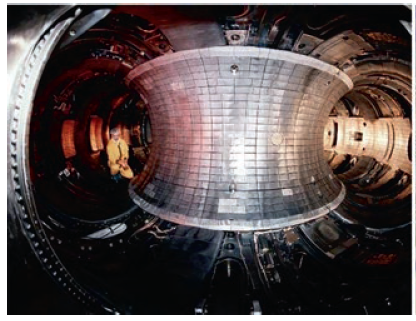
\includegraphics[width=\textwidth]{TokamakVessel.png}
\end{minipage}
\begin{minipage}{0.49\textwidth}
  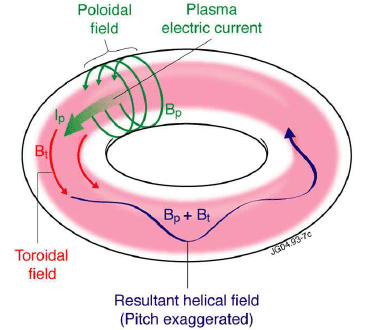
\includegraphics[width=\textwidth]{Toroidal-magnetic-field-B-t.png}
\end{minipage}
    \caption[Donut-shaped Tokamak and magnetic field]{Donut-shaped Tokamak along with toroidal and poloidal. In such device, plasma is confined and accelerated by a toroidal magnetic field just surrounding the 'donut' penetrating from its hole. Then plasma travel along the 'donut' in circle. The motion of ions in plasma forms another poloidal magnetic field further confine them within the core of the elliptic shape of a vertical slice. The 'donut-shaped' is designed in purposes. The right-hand image shows the  The images is adopted from \cite{moynihan2023fusion} and \cite{twarog2011test}. }
    \label{fig:TokamakDonut}
\end{figure}
\begin{figure}
    \centering
    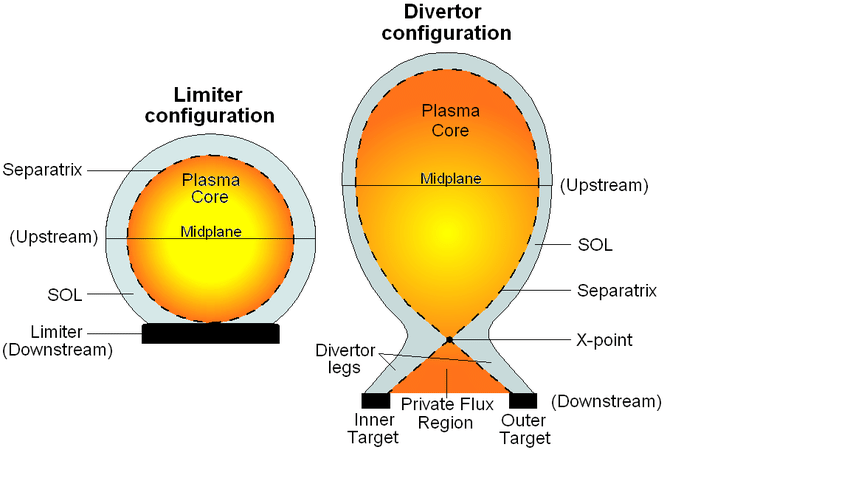
\includegraphics[width=0.5 \textwidth]{Chapter2/Figs/limiter_and_divertor.png}
    \caption[Limiter and divertor in tokamaks]{Limiter and divertor in tokamaks. They are used to protect the walls from plasma erosion. This plot is adopted from \cite{kumar2021analysis}.}
    \label{fig:LimiterDivertor}
\end{figure}


\subsection{Hydrodynamic Effects}
\label{section2.3.1}
In the Euler system without a magnetic field, we apply the reflective boundary condition \cite{sambasivan2009ghost} on the rigid body. Given $\mathbf{v}$ is the velocity vector of the plasma and $\mathbf{U}$ is the velocity vector of the rigid body. We are analyzing on a boundary point with a unit normal vector $\mathbf{n}$. For a normal velocity, it should obey the no-penetration:
$$v_n=U_n.$$ The $v_n=\mathbf{v}\cdot\mathbf{n}$ and $U_n=\mathbf{U}\cdot\mathbf{n}$ are the normal velocities of the plasma and the rigid body on the boundary. For a fixed rigid body $U_n=0$. In a two-dimensional system, the tangential velocity should obey a slip condition:$$\partial v_t /\partial \mathbf{n} =0$$ or a no-slip condition: $$v_t =U_t,$$where $v_t$ and $U_t$ are the tangential components and $\partial v_t /\partial \mathbf{n}$ is its partial derivative . Since the viscosity of ideal plasma is zero, we mainly apply the slip condition. 

Such boundary conditions can be described as Neumann type conditions or Dirichlet type conditions \cite{arendt2004dirichlet}. For a variable $\phi$, they are 
\begin{align*}
    \text{Neumann boundary condition: } \quad &\partial \phi/\partial \mathbf{n} =constant \quad&\text{on boundary}\\
     \text{Dirichlet boundary condition: } \quad&\phi =constant \quad&\text{on boundary}
\end{align*}
To be specific, when we have set value of a variable on boundary, it satisfies the Dirichlet condition; when we have a normal derivative on boundary, it satisfies Neumann condition. Hence, tangential velocity with slip condition satisfies the Neumann boundary condition and normal velocity with no-penetration condition satisfies the Dirichlet condition. The other scalar variables in the Euler system also satisfy the Neumann condition with zero derivative along the normal vector, $\partial \cdot/\partial \mathbf{n}=0$.

\subsection{Magnetic Effects}
There are mainly three kinds of boundary conditions for the magnetic field: perfect conducting wall, insulating wall, and resistive wall.
\subsubsection{Perfect Conducting Wall}
A necessary condition for a perfect conductor is \cite{yanagisawa1991fixed,ju2023incompressible}: $$\mathbf{n}\times\mathbf{E}=0.$$ This is because on a perfect conductor, there is no electric potential difference. According to Faraday's law, the first equation in Maxwell's equations in section~\ref{section2.1}, $\frac{\partial \mathbf{B}}{\partial t} + \nabla \times\mathbf{E} = 0$. Since we are dealing with a fixed rigid body, a normal vector on the boundary is not a function of $t$, $\partial \mathbf{n}/\partial t=0$. Furthermore, $\mathbf{n}\cdot\left(\nabla\times\mathbf{E}\right)=\nabla\cdot\left(\mathbf{n}\times\mathbf{E}\right)=0$. We have an inner product for Faraday's Law:
$$\mathbf{n}\cdot(\frac{\partial \mathbf{B}}{\partial t} + \nabla \times\mathbf{E})=\frac{\partial \left(\mathbf{n}\cdot\mathbf{B}\right)}{\partial t}= 0.$$
This means that on the perfect conducting boundary, normal component of magnetic field only depends on the initial values, given $B_n=\mathbf{B}\cdot\mathbf{n}=B_{n0}$. This forms a 'no-penetration' condition \cite{clauser2021iter} for the normal magnetic field similar to the normal velocity in section ~\ref{section2.3.1}. A perfect conductor will not affect the tangential magnetic field $B_t$. A 'slip' condition is also preserved in the tangential field. In this condition, the normal magnetic field satisfies the Dirichlet boundary condition $B_n=B_{n0}$, and the tangential field satisfies the Neumann boundary condition $\partial B_t/\partial \mathbf{n}=0$.
\subsubsection{Insulating Wall}
An insulator means that no induced magnetic field will be generated inside it. Hence, the magnetic field should be a constant vector along the normal vector. A mathematical description \cite{freidberg2014ideal} for an insulator is:
\begin{align*}
\nabla \times \mathbf{B} &= 0 \\
\nabla \cdot \mathbf{B} &= 0.
\end{align*}
In this situation, both the normal and tangential components of the magnetic field satisfy the Neumann boundary condition $\partial B_t/\partial \mathbf{n} = \partial B_n/\partial \mathbf{n} = 0$.
\subsubsection{Resistive Wall}
A resistive wall can be regarded as an intermediate state between a perfect conducting wall and an insulating wall. A perfect conductor equivalently has infinite conductivity or zero resistivity, while an insulator equivalently has zero conductivity or infinite resistivity. A resistive wall lies in between, with finite conductivity and finite resistivity. The magnetic field is fully reflected by a perfect conducting wall and easily penetrates an insulator. However, with finite resistivity, it penetrates a resistive wall slowly \cite{bondeson2003physics}. The larger the resistivity, the more the penetration. Modeling a resistive wall is inherently more complex than modeling a perfect conductor or an insulator. The preliminary results in this report are all using a perfect conducting wall. Simulations with resistive walls will be considered in the next part of this project and included in the next report.
\subsubsection{Actual Boundary on Tokamak}
The most ideal boundary is the perfect conducting wall. The fully induced reflected magnetic field provides a strong force of passive feedback for stabilizing the plasma \cite{takeda1991computation,clauser2021iter,bondeson2003physics,yolbarsop2022analytic,bondeson1994stabilization}. Between the core plasma and the wall, the outside fixed rigid body, there is sparse plasma with much lower density, which can be regarded as a vacuum \cite{clauser2021iter,takeda1991computation}. As long as the perfect conducting wall is close enough to the plasma, it remains stable. This vacuum region can be regarded as an insulator. Both models of a fixed perfect conducting wall and a vacuum free boundary space are used in computational models of tokamak devices \cite{clauser2021iter,freidberg2014ideal}. However, the actual walls of tokamaks have finite conductivity. A more realistic scenario replaces the perfect conducting wall with a resistive wall \cite{clauser2021iter}. The resistivity reduces the model's stability, where the external modes start to grow \cite{haney1989variational,bondeson2003physics,bondeson1994stabilization}. A resistive plasma further increases the modeling complexity \cite{yolbarsop2022analytic}.

Our project mainly models the ideal plasma with no resistivity and viscosity under a perfect conducting fixed rigid body and then generalizes it to a resistive model.
%!TEX root = ../thesis.tex
%*******************************************************************************
%*********************************** First Chapter *****************************
%*******************************************************************************

\chapter{Numerical Methods}  %Title of the First Chapter

\ifpdf
    \graphicspath{{Chapter3/Figs/Raster/}{Chapter3/Figs/PDF/}{Chapter3/Figs/}}
\else
    \graphicspath{{Chapter3/Figs/Vector/}{Chapter3/Figs/}}
\fi

\label{chapter 3}

%**************************************************************************
Building on the theoretical framework established in Chapter 2, we now shift our focus to the numerical methods used to simulate the behavior of plasma in tokamaks. Chapter 3 will detail the specific numerical schemes and techniques employed in our simulations, including the MUSCL-Hancock and MHD-HLLC methods. We will also discuss advanced techniques for divergence cleaning and the handling of rigid body interactions within the plasma. These methods are critical for ensuring the accuracy and stability of our simulations, which are validated through various tests and preliminary results presented in the following chapter.
\section{Numerical Scheme}
\label{section 3.1}
We establish a two-dimensional Cartesian grid and then apply a finite volume method to it. We use a CFL number of $C_{CFL}=0.4$ for two-dimensional space and a dimensional splitting operator $\mathbf{u}_{i,j}^{n+1}={{Y}^{\left( \Delta t/2 \right)}}{{X}^{(\Delta t)}}{{Y}^{\left( \Delta t/2 \right)}}\left( \mathbf{u}_{i,j}^{n} \right)$. The CFL number, $C_{CFL}$, stands for the Courant–Friedrichs–Lewy (CFL) number, which is used to calculate the maximum stable time step for each iteration. For stability, $C_{CFL}$ should be in the range $(0, 1)$ and should not be bigger than 1 in normal cases. This is used to calculate the time steps two-dimensionally computationally through $\Delta t=\frac{C_{CFL} \min(\Delta x, \Delta y)}{a}$, where $a$ is the fastest wave speed. In our case, the fastest wave $a$ is calculated by $a=\max(|v_x|,|v_y|)+c_f$. $c_f$ is the fast magneto-acoustic speed
$$c_f=\sqrt{\frac{1}{2}(c_s^2+c_a^2+(c_s^2+c_a^2)^2-4c_s^2c_a^2cos^2\theta)},$$ where $\theta$ is its propagation direction. $c_a^2 \cos^2 \theta = B_x^2 / \rho$ when updating in the x direction and $c_a^2 \cos^2 \theta = B_y^2 / \rho$ when updating in the y direction. The Alfvén wave speed and the acoustic speed are calculated by $c_a = \frac{|\mathbf{B}|}{\sqrt{\rho}}$ and $c_s = \sqrt{\frac{\gamma p}{\rho}}$. Specifically, when the magnetic field is zero $\mathbf{B}=0$, the fast magneto-acoustic speed equals to the acoustic speed $c_f = c_s$. Here we use a relstive low $C_{CFL}=0.4$ originally to suppress the potential oscillations when waves propagate obliquely. we found that using a higher CFL number, such as 0.8, will also works. The ${X}^{(\Delta t)}$ and ${Y}^{(\Delta t)}$ are the operators that evolve the equation using the conservative update formula (\ref{MHDsystem}) within the time step $\Delta t$ in each direction. They are given by:
\begin{align*}
&{X}^{(\Delta t)}(\mathbf{u}^{n}_{i}) = \mathbf{u}^{n}_{i} - \frac{1}{2} \frac{\Delta t}{\Delta x} \left( \mathbf{f}_{i+1/2}^{n} - \mathbf{f}^{n}_{i-1/2} \right)\ &\text{operator updating in the x direction,}\\
&{Y}^{(\Delta t)}(\mathbf{u}^{n}_{i})= \mathbf{u}^{n}_{i} - \frac{1}{2} \frac{\Delta t}{\Delta y} \left( \mathbf{g}_{i+1/2}^{n} - \mathbf{g}^{n}_{i-1/2} \right)\ &\text{operator updating in the y direction.}
\end{align*}
$\mathbf{f}$ and $\mathbf{g}$ are the fluxes in the x and y directions. The numerical scheme we use to calculate the flux $\mathbf{f}$ or $\mathbf{g}$ is the MUSCL-Hancock method \cite{toro2013riemann} along with the MHD-HLLC solver \cite{li2005hllc}.
\subsection{MUSCL-Hancock}
We use a MUSCL-Hancock method to achieve second-order accuracy in time and space \cite{toro2013riemann}. This method generalizes a first-order finite volume scheme, in our case MHD-HLLC, to second-order accuracy. 
The MUSCL-Hancock method initiates with the MUSCL step, a technique proposed by van Leer \cite{van1979towards}, which is an acronym for Monotonic Upstream-Centered Scheme for Conservation Laws. This method employs linear reconstruction strategies to attain second-order spatial accuracy, effectively leveraging the differences between cell values, denoted as $\Delta_{i+1/2}=\mathbf{u}_{i+1}-\mathbf{u}_i$. Consequently, a slope within cells can be calculated using $\Delta_i=\frac{1}{2}(1+\omega)\Delta_{i-1/2}+\frac{1}{2}(1-\omega)\Delta_{i+1/2}$. Here, $\omega$ serves as a balancing coefficient between minimizing oscillation and enhancing capture, which is crucial for the scheme's upwind bias \cite{li2019weno}. For Euler and MHD cases, a $\omega$ value of 0 is typically chosen to ensure stability. The value of $\mathbf{u}_{i}(x)$ within a cell is determined by $\mathbf{u}_{i}(x)=\mathbf{u}_{i}^n+(x-x_i)\frac{\Delta_i}{\Delta x}$, with $x_i$ representing the cell's center. Slope limiting introduces a limiter to the slope to prevent excessive gradients, defined as ${{\mathbf{\bar{u}}}_{i}}(x)=\mathbf{u}_{i}^{n}+(x-{{x}_{i}})\frac{{\bar{\Delta}}_{i}}{\Delta x}$, where ${{\bar{\Delta }}_{i}}=\xi (r){{\Delta }_{i}}$, and $\xi(r)$ is the applied limiter. The slope limiter used is the Van-Leer limiter \cite{van1979towards}, given by $$\xi(r) = 
\begin{cases} 
0 & r \leq 0 \\
\min\left( \frac{2r}{1+r}, \xi_R(r) \right) & r > 0 
\end{cases}$$, with $r = \frac{\Delta_{i-\frac{1}{2}}}{\Delta_{i+\frac{1}{2}}}=\frac{q_i-q_{i-1}}{q_{i+1}-q_i}, \quad \xi_R(r) = \frac{2}{1+r}
$. Through the MUSCL step, the method facilitates a controlled slope within cells to achieve second-order spatial accuracy. Specifically, it adjusts $$\mathbf{\bar{u}}_i^{R,L}=\mathbf{u}_i\pm \frac{1}{2}\bar{\Delta}_i$$ $$\quad \mathbf{\bar{u}}_{i+1}^{R,L}=\mathbf{u}_{i+1}\pm \frac{1}{2}\bar{\Delta}_{i+1}$$, thereby enabling enhanced accuracy within the numerical scheme.

The Hancock step is utilized to predict the cell interface states at the half-time step, thereby achieving temporal second-order accuracy. In practice, it facilitates in x direction $$\mathbf{\bar{u}}^{L,n+\frac{1}{2}}_{i+1} = \mathbf{\bar{u}}^{L}_{i+1} - \frac{1}{2} \frac{\Delta t}{\Delta x} \left( \mathbf{f}(\mathbf{\bar{u}}^{R}_{i+1}) - \mathbf{f}(\mathbf{\bar{u}}^{L}_{i+1}) \right),$$
$$\mathbf{\bar{u}}^{R,n+\frac{1}{2}}_{i} = \mathbf{\bar{u}}^{R}_{i} - \frac{1}{2} \frac{\Delta t}{\Delta x} \left( \mathbf{f}(\mathbf{\bar{u}}^{R}_{i}) - \mathbf{f}(\mathbf{\bar{u}}^{L}_{i}) \right).$$


\subsection{MHD-HLLC}
The MHD-HLLC solver is originally developed from HLL solver. The HLL approximate Riemann solver was devised by Harten, Lax, and van Leer (HLL) \cite{harten1983upstream}. The HLL method considers an approximation where only two shock waves emerge from a discontinuity, a two-wave model using the two largest signal speeds for bounding. Between these two shocks, there is a homogeneous intermediate state that can be solved using the Rankine-Hugoniot conditions for these two shocks. Such an intermediate state may be too diffusive, neglecting intermediate characteristic fields \cite{toro2019hllc}, such as contact surfaces or shear waves. The assumption of HLL is only appropriate for a hyperbolic system like one-dimensional compressible Euler equations. Toro \textit{et al.} further improved this method by proposing a three-wave model, the HLLC approximate Riemann solver. This considers another intermediate wave, like a contact discontinuity, between these two shocks, separating the intermediate state, with 'C' standing for contact discontinuity \cite{toro1994restoration,toro2013riemann,toro2019hllc}. The HLLC approximate solver greatly enhances the resolution and is extremely popular.

Meanwhile, an MHD extension for HLL, MHD-HLL, was proposed by Janhunen \cite{janhunen2000positive}. This method maintains positivity by allowing small violations of $\nabla\cdot\mathbf{B}=0$. Like HLL, MHD-HLL is too diffusive. Li \cite{li2005hllc} combined the advantages of the MHD-HLL solver and the HLLC approximate Riemann solver and proposed MHD-HLLC. This significantly increases the resolution. However, this method considers a homogeneous magnetic field level and uses an HLL solver for the magnetic field \cite{miki2007large}. The MHD-HLLC approximate solver has not yet considered the characteristic field magnetically, like the rotational discontinuity of the Alfvén waves. Nonetheless, the MHD-HLLC method combines the advantages of the HLLC approximate solver and the MHD-HLL solver. In general, it strikes a good balance between robustness and accuracy. We primarily use the MHD-HLLC approximate solver as our MHD solver fellowing Li \cite{li2005hllc}.

The MHD-HLLC approximate solver posits that a discontinue problem encompasses only three waves: two shock waves and a middle contact discontinuity. In our computational practical, we use this method on finding a solution based on these two states $\mathbf{\bar{u}}^{L,n+\frac{1}{2}}_{i+1}$ and $\mathbf{\bar{u}}^{R,n+\frac{1}{2}}_{i}$, derived from the MUSCL-Hancock step. We take $x$ direction as example. Those fluxes on y are similer. Two estimated shock wave speeds in the $x$ direction, ${{S}_{L}}$ and ${{S}_{R}}$, are calculated in our scheme by $${{S}_{L}}=\min \left(  {{v}_{x,L}} , {{v}_{x,R}}  \right)-\max \left( {{c}_{f,x,L}},{{c}_{f,x,R}} \right),$$ $${{S}_{R}}=\max \left(  {{v}_{x,L}} , {{v}_{x,R}}  \right)+\max \left( {{c}_{f,x,L}},{{c}_{f,x,R}} \right).$$ Here, ${c}_{f,x,L}$ denotes the fast magneto-acoustic speed calculated from the left state. The calculation of fast magneto-acoustic speed is discussed in the beginning of this section \ref{section 3.1}. For the Euler part, Toro \textit{et al.} \cite{toro2013riemann} gave implementation details for HLLC. On the magnetic field, utilizing $\mathbf{B}^{HLLC}=\mathbf{B}^{HLL}$ \cite{li2005hllc} allows for the updating flux calculation: $$\mathbf{f_{i+\frac{1}{2}}}=\mathbf{f^{HLLC} \left( \mathbf{\bar{u}}^{R,n+\frac{1}{2}}_{i},\mathbf{\bar{u}}^{L,n+\frac{1}{2}}_{i+1} \right) }.$$
These generate a computational flux which can be utilized on the updating operator $X^{(\Delta t)}$.
 

\section{Divergence Cleaning Technique}
In section ~\ref{section 2.2}, we discuss several divergence cleaning methods and constrained transport, concluding that a mixture of hyperbolic and parabolic divergence cleaning is accurate enough for our case \cite{vides2013divergence}. We use this divergence cleaning as additional equations evolving alongside the MHD equations. The governing equations are:
\begin{align*}
\frac{\partial \mathbf{B}}{\partial t} +  \nabla \psi = 0 \\
D(\psi) + \nabla \cdot \mathbf{B} = 0
\end{align*}, where a hyperbolic/parabolic operator is 
\begin{equation*}
D(\psi) = \frac{1}{c_h^2} \frac{\partial \psi}{\partial t} + \frac{1}{c_p^2} \psi.
\end{equation*}
The equation for $\psi$ becomes 
\begin{equation*}
\frac{1}{c_h^2} \frac{\partial \psi}{\partial t} + \frac{1}{c_p^2} \psi+ \nabla \cdot \mathbf{B} = 0 .
\end{equation*}
Hence, this forms a hyperbolic system for $\psi$ and $\mathbf{B}$ with a source term
\begin{align*}
\frac{\partial \psi}{\partial t}+c_h^2\nabla \cdot \mathbf{B}&=-\frac{c_h^2}{c_p^2}\psi\\
\frac{\partial \mathbf{B}}{\partial t} +  \nabla \psi &= 0
\end{align*}
The numerical equation for a two-dimensional grid is :
\begin{equation}
    {{\mathbf{U}}_{t}}+\mathbf{f}_x{{(\mathbf{U})}}+\mathbf{g}_y{{(\mathbf{U})}}=\mathbf{S},
\end{equation}
where 
\[
\mathbf{U} = \begin{bmatrix}
\psi \\
B_x \\
B_y
\end{bmatrix}, \quad
\mathbf{f} = \begin{bmatrix}
c_h^2B_x \\
\psi \\
0
\end{bmatrix}, \quad
\mathbf{g} = \begin{bmatrix}
c_h^2B_y \\
0 \\
\psi
\end{bmatrix}, \quad
\mathbf{S}=\begin{bmatrix}
-\frac{c_h^2}{c_p^2} \psi \\
0 \\
0
\end{bmatrix}
.\] We use a Godunov scheme flux to update this equation. Take the flux in x direction as an example:
\begin{equation*}
\mathbf{f}_{i+1/2}=\begin{bmatrix}
0.5c_h(\psi_i-\psi_{i+1})+0.5c_h^2(B_{x,i}+B_{x,i+1}) \\
0.5c_h(B_{x,i}-B_{x,i+1})+0.5(\psi_i+\psi_{i+1})\\
0
\end{bmatrix}.
\end{equation*}

\section{Technique for Rigid Body}
We employ the level set method \cite{andrew2000level} to define the boundaries of rigid bodies. The boundary is specified by setting the zeros of the level set function $\phi$ in the level set method. For the geometries, all we need for iteration are the signed distance, the value of the level set function, and the closest normal vectors. Computationally, we achieve this by giving those closest boundary-pass-by cells an initial $\phi$ and normal vector $\mathbf{n}$ pointing to the closest boundary. Then a fast marching method can be applied to find a plausible $\phi$ and normal vector $\mathbf{n}$ for every cell by iterating through the whole mesh in fictitious time to solve an Eikonal equation $|\nabla\phi|=1$. The normal vector is inherited from the affecting point during the iteration. Hence, the distances and normal vectors are prepared for updating.

After applying the level set method, reflective boundary conditions are then applied to ghost cells that are sufficiently close, specifically where the absolute value of the level set function is less than $GhostCells \times \max(\Delta x, \Delta y)$. The required number of ghost cells, denoted as $GhostCells$, depends on the finite volume scheme utilized. For the MUSCL-Hancock scheme used in our study, we need at least $GhostCells \ge 2$. In our work, the method we used to apply the reflective boundary condition is heavily inspired by Sambasivan \textit{et al.} \cite{sambasivan2009ghost}. We acknowledge and appreciate the significant contributions of their research, which have provided a foundational basis for our implementation.
\subsubsection{Interpolation} For each ghost cell, we need a reflected point as demonstrated in Figure~\ref{fig:Reflective Boundary Condition}. In the figure, the variables at IP1 are needed. The position of IP1, $\mathbf{X}_{IP1}=(x_{IP1},y_{IP1})^T$, can be calculated by the position of P $\mathbf{X}_P=(x_{P},y_{P})^T$, the absolute value of level set function $\left| {{\phi }_{P}} \right|$ and its unit normal vector $\mathbf{N}_P$ \cite{sambasivan2009ghost}:
$$\mathbf{X}_{IP1}=\mathbf{X}_P+2\left| {{\phi }_{P}} \right|\mathbf{N}_P.$$
\begin{figure}
    \centering
    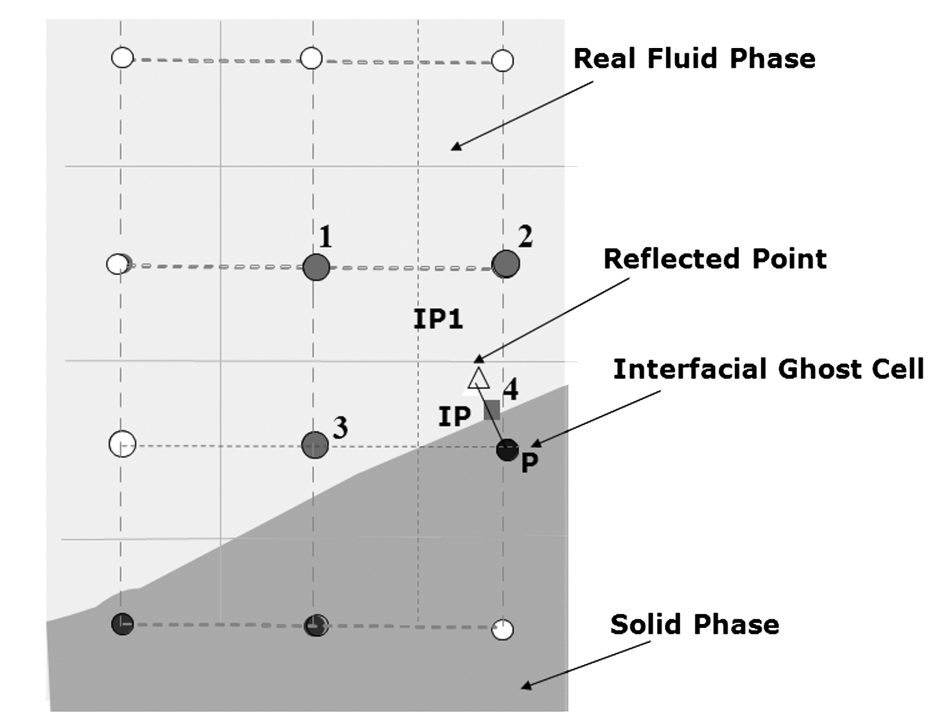
\includegraphics[width=0.5\linewidth]{ReflectiveBC.png}
    \caption[Reflective Boundary Condition]{Reflective Boundary Condition with Bilinear Interpolation Procedure. The reflective boundary condition is applied at point P, requiring variables from the reflected point IP1. Bilinear interpolation necessitates the variables from ghost cell P, where the variables from nearest boundary point IP are instead used. The variables at IP are determined by either Neumann or Dirichlet boundary conditions. This plot is adopted from \cite{sambasivan2009ghost}.}
    \label{fig:Reflective Boundary Condition}
\end{figure}
When interpolating a specific variable $\zeta$ on IP1, the interpolation has the form:
$$\zeta_{IP1}(x_{IP1},y_{IP1})=a_1+a_2x_{IP1}+a_3y_{IP1}+a_4x_{IP1}y_{IP1}.$$
The interpolation points $i=1,2,3,4$ must also satisfy this function with $\zeta_{i}(x_{i},y_{i})=a_1+a_2x_{i}+a_3y_{i}+a_4x_{i}y_{i}.$ Hence, the coefficients $a_{1\sim4}$ can be derived from solving a linear algebra equation:
$$\begin{bmatrix}
    1&x_1&y_1&x_1y_1\\1&x_2&y_2&x_2y_2\\1&x_3&y_3&x_3y_3\\1&x_4&y_4&x_4y_4\\
\end{bmatrix}\begin{bmatrix}
    a_1\\a_2\\a_3\\a_4
\end{bmatrix}=\begin{bmatrix}
    \zeta_{1}\\\zeta_{2}\\\zeta_{3}\\\zeta_{4}
\end{bmatrix}.$$ 
\subsubsection{Handling Invalid Ghost Cells in Interpolation}Some of the necessary points may be the invalid ghost cells. In our case in Figure \ref{fig:Reflective Boundary Condition}, the point 4 is exactly the ghost cell P. In this situation, the closest boundary point IP substitutes. We need to find another equation for IP. Recall the Neumann boundary condition and Dirichlet boundary condition in section \ref{section2.3.1}. When $\zeta$ satisfies the Dirichlet boundary condition of $\zeta_{IP}=\zeta_D$ on boundary $\mathbf{X}_{IP}=(x_{IP},y_{IP})$, we have $$\zeta_{D}=a_1+a_2x_{IP}+a_3y_{IP}+a_4x_{IP}y_{IP}.$$ This gives the linear algebra equation
$$\begin{bmatrix}
    1&x_1&y_1&x_1y_1\\1&x_2&y_2&x_2y_2\\1&x_3&y_3&x_3y_3\\1&x_{IP}&y_{IP}&x_{IP}y_{IP}\\
\end{bmatrix}\begin{bmatrix}
    a_1\\a_2\\a_3\\a_4
\end{bmatrix}=\begin{bmatrix}
    \zeta_{1}\\\zeta_{2}\\\zeta_{3}\\\zeta_{D}
\end{bmatrix}.$$
When $\zeta$ satisfies the Neumann boundary condition of $\partial\zeta_{IP}/\partial\mathbf{n}=\zeta_N$, we have \begin{align*}\frac{\partial\zeta_{IP}}{\partial\mathbf{n}}=\frac{\partial\zeta_{IP}}{\partial x}n_x+\frac{\partial\zeta_{IP}}{\partial y}n_y=\zeta_{N}\\
\zeta_{IP}=a_1+a_2x_{IP}+a_3y_{IP}+a_4x_{IP}y_{IP},
\end{align*}
where $\mathbf{n}=(n_x,n_y)^T$. The partial derivative for $\zeta_{IP}$ gives
$$0+a_2n_x+a_3n_y+a4(n_xy_{IP}+n_yx_{IP})=\zeta_{N}$$ and the linear algebra form 
$$\begin{bmatrix}
    1&x_1&y_1&x_1y_1\\1&x_2&y_2&x_2y_2\\1&x_3&y_3&x_3y_3\\0&n_x&n_y&n_xy_{IP}+n_yx_{IP}\\
\end{bmatrix}\begin{bmatrix}
    a_1\\a_2\\a_3\\a_4
\end{bmatrix}=\begin{bmatrix}
    \zeta_{1}\\\zeta_{2}\\\zeta_{3}\\\zeta_{N}
\end{bmatrix}.$$
\subsubsection{Applying Boundary Condition}
After the interpolation, we can derive the variables on ghost cell P from the reflected point IP1 based on the boundary conditions discussed in section \ref{section2.3.1}. A reflective boundary condition is applied to the velocity field where averages on the boundary are $U_n$ and $U_t$ normally and tangentially:
\begin{align*}
v_{n,P} &= 2U_n - v_{n,IP1} \\
v_{t,P} &= 2U_t - v_{t,IP1}
\end{align*}
For a fixed rigid body, $U_n = 0$. For an ideal plasma with no viscosity, under the slip condition, $U_t = v_{t,IP1}$.

For the magnetic field, if the rigid body is regarded as a perfect conductor, the normal magnetic field and tangential field should satisfy the Dirichlet boundary condition with $B_n = B_{n0}$ and the Neumann boundary condition $\partial B_t / \partial \mathbf{n} = 0$, similar to the 'no-penetration' and 'slip' conditions. Hence,
\begin{align*}
B_{n,P} &= 2B_{n0} - B_{n,IP1} \\
B_{t,P} &= B_{t,IP1}.
\end{align*}
If the rigid body is regarded as an insulator, both the normal component and the tangential component satisfy the Neumann condition:
\begin{align*}
B_{n,P} &= B_{n,IP1} \\
B_{t,P} &= B_{t,IP1}.
\end{align*}
The other scalar variables satisfy the Neumann condition with zero derivatives and are just copies from the reflected point.
%!TEX root = ../thesis.tex
%*******************************************************************************
%*********************************** First Chapter *****************************
%*******************************************************************************

\chapter{Validation Test and Preliminary Results}  %Title of the First Chapter

\ifpdf
    \graphicspath{{Chapter4/Figs/Raster/}{Chapter4/Figs/PDF/}{Chapter4/Figs/}}
\else
    \graphicspath{{Chapter4/Figs/Vector/}{Chapter4/Figs/}}
\fi

\label{chapter 4}


%**************************************************************************
In this chapter, we conduct several tests to validate the methods discussed above. The tests include the Orszag-Tang test, which validates the MHD solver and divergence cleaning; shock diffraction over a wedge/cylinder for rigid body geometries; and rotated Sod/Brio-Wu tests for outside rigid body and MHD boundary conditions.
\section{Orszag-Tang Test}
In our study, we have employed an MHD-HLLC MHD solver. To achieve second-order accuracy, the MUSCL-Hancock method has been utilized. Furthermore, to ensure the magnetic field remains divergence-free, a mixed hyperbolic/parabolic GLM divergence cleaning method has been applied. These are discussed in Chapter 3. We are using the Orszag-Tang test to validate these methods. The initial data of Orszag-Tang test is given in the Table \ref{tab:OrszagTangInitial}. The Orszag-Tang test is conducted within a spatial domain of $[0,1] \times [0,1]$ with a resolution of $256 \times 256$, employing periodic boundaries surrounding the domain. Results are analyzed at $t=0.5s$ and $t=1.0s$, under the conditions of ideal plasma with $\gamma = 5/3$. The results, depicted in Figures \ref{fig:OT}, align closely with those in Vides \textit{et al.} \cite{vides2013divergence}. However, certain discrepancies remain. These can primarily be attributed to differences in the MHD solvers utilized. Specifically, our solver employs the MHD-HLLC method, whereas Vides \textit{et al.} use the HLLD solver. This variation in methodology could account for the observed differences in results. Miki \textit{et al.} also use MHD-HLLC solver on conducting Orszag-Tang test shown on the right in Figure \ref{fig:OTComparing}. Our result is similar to theirs which validate our MHD-HLLC solver. We have The application of mixed divergence cleaning reduces diffusion and error spread significantly, as demonstrated in Figure \ref{fig13:OrszagtangDiv}. The divergence range is reduced from  [-25,30] to [-5,4].
\begin{table}[H]
\caption{Initial data for the Orszag-Tang test. }
\label{tab:OrszagTangInitial}
\centering 
\begin{tabularx}{0.8\textwidth}{@{}cccccccc@{}}
\toprule
$\rho$ & $v_x$ & $v_y$ & $v_z$  & $B_x$ & $B_y$ & $B_z$ & $p$ \\
\hline
$\gamma^2$ & $-\sin(2\pi y)$ & $\sin(2\pi x)$ & 0.0 & $-\sin(2\pi y)$ & $\sin(4\pi x)$ & $0.0$ & $\gamma$ \\
\bottomrule
\end{tabularx}
\end{table}

\begin{figure}[htbp]
\centering
\begin{minipage}[OrszagTang_mine]{0.45\textwidth}
  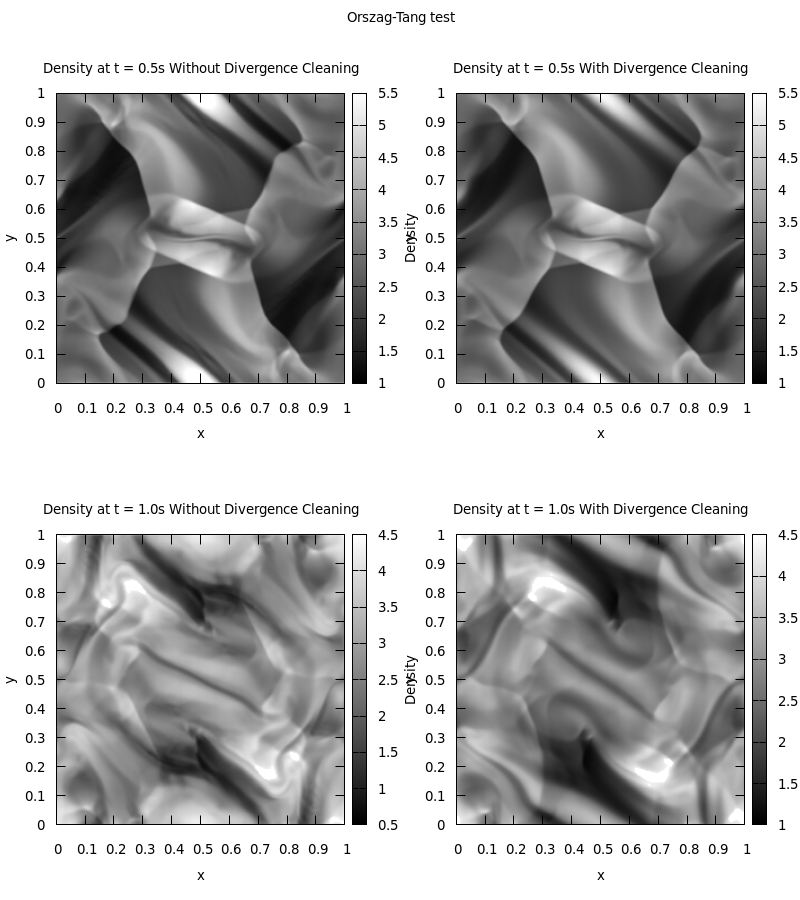
\includegraphics[width=\textwidth]{OrszagTang.png}
\end{minipage}
\begin{minipage}[OrszagTang_noDC_vides]{0.235\textwidth}
  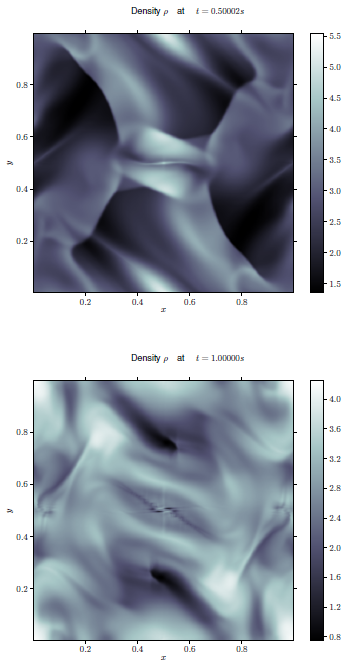
\includegraphics[width=\textwidth]{OT_no_vides.png}
\end{minipage}
\begin{minipage}[OrszagTang_yesDC_vides]{0.235\textwidth}
  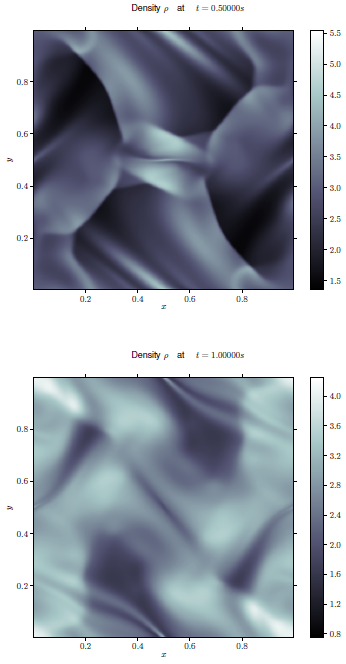
\includegraphics[width=\textwidth]{OT_yes_vides.png}
\end{minipage}
\caption[OrszagTang test]{The results of Orszag-Tang test. The left side shows our simulation results, and the right side shows the results from Vides \textit{et al.} \cite{vides2013divergence}.}
\label{fig:OT}
\end{figure}

\begin{figure}[htbp]
    \centering
    \begin{minipage}{0.45\textwidth}
  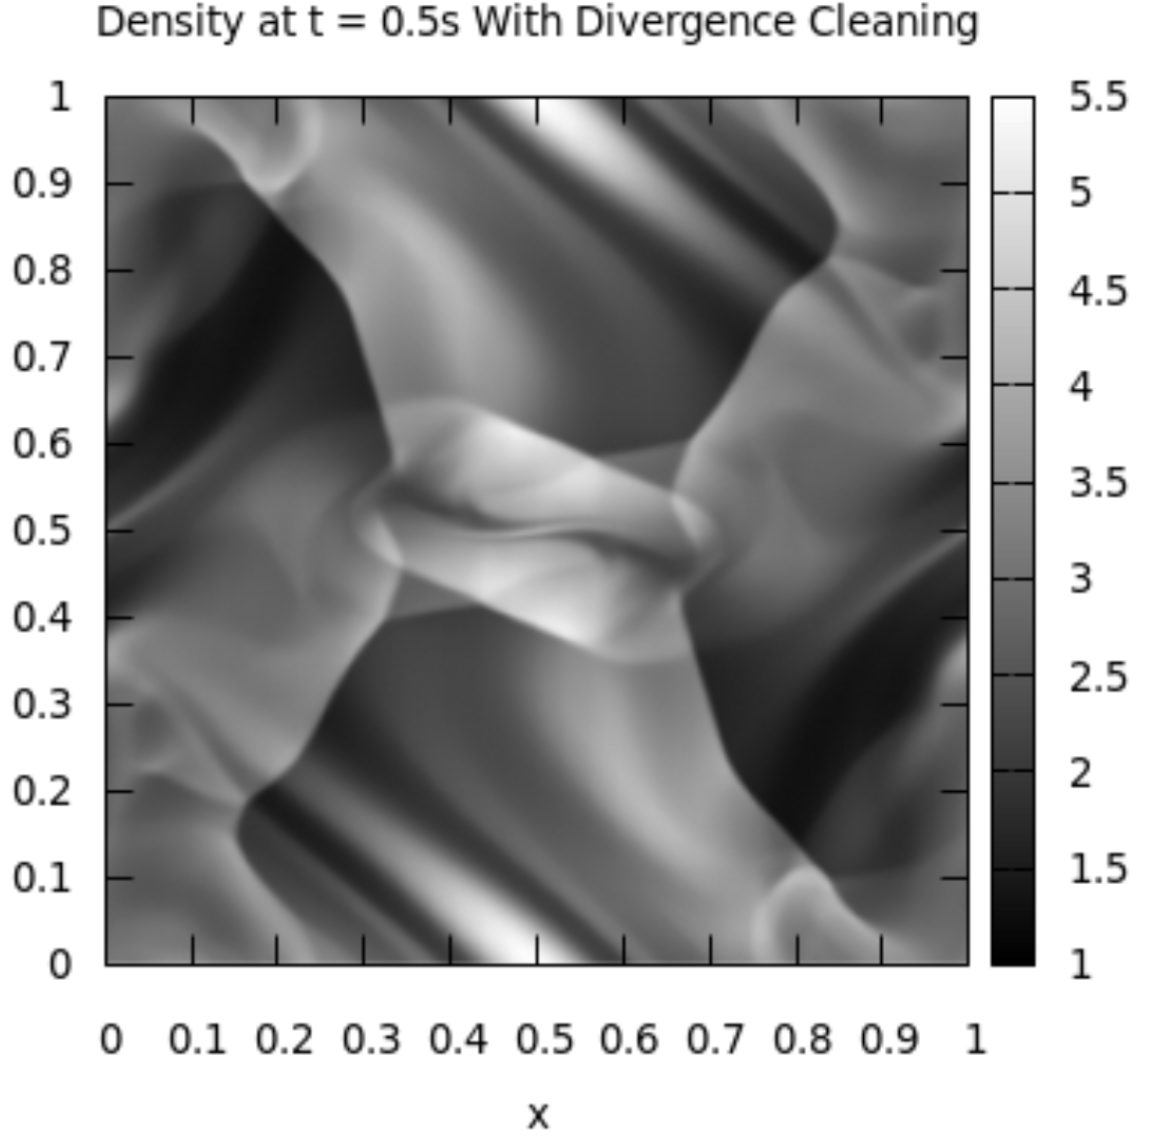
\includegraphics[width=\textwidth]{OT_mine.png}
\end{minipage}
\begin{minipage}{0.43\textwidth}
  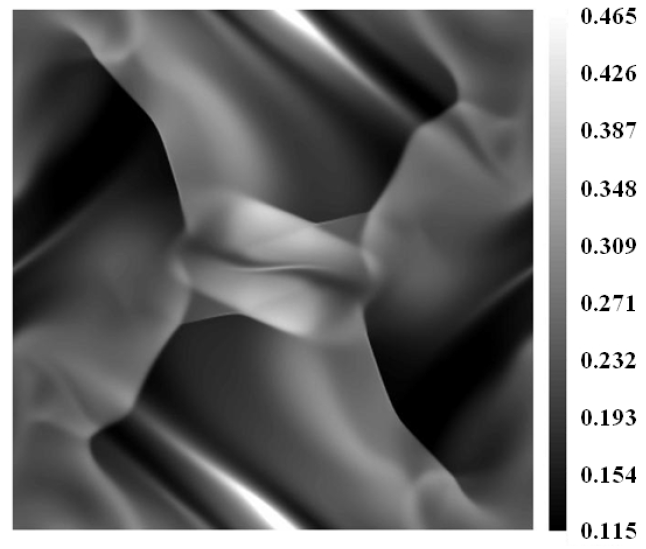
\includegraphics[width=\textwidth]{OT_Miki.png}
\end{minipage}
    \caption[Orszag-Tang with HLLC method]{Comparing the results of Orszag-Tang test with same MHD-HLLC solver. The left image shows our result produced with MHD-HLLC solver at $t=0.5$. The image on the right demonstrates the corresponding result from Miki \textit{et al.} \cite{miki2007large}. These two images look almost the same except for the different range of colorbox and resolution, which validate our MHD-HLLC method.}
    \label{fig:OTComparing}
\end{figure}

\begin{figure}[htbp]
    \centering
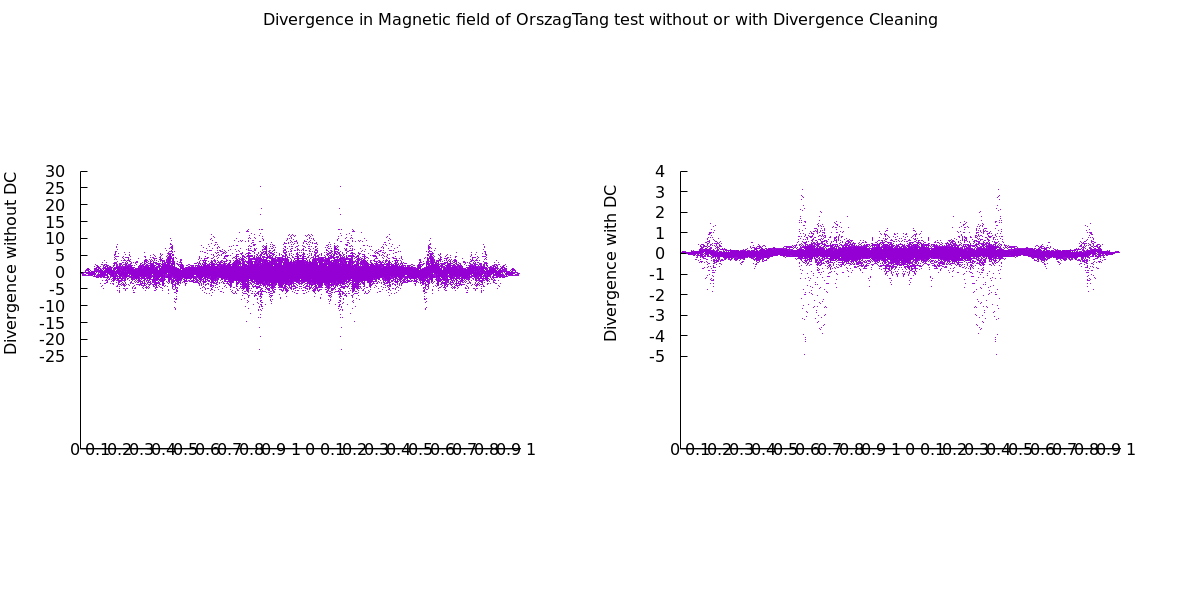
\includegraphics[width=0.9\textwidth]{OrszagTangDiv.png}
    \caption[Divergence in OrszagTang]{Divergence in the magnetic field in Orszag-Tang tests without divergence cleaning (left) and with divergence cleaning (right). These diagonal plots demonstrate the efficiency of mixed divergence cleaning. The range of divergence is reduced from [-25,30] to [-5,4]. After applying the cleaning, data points lay closer to the zero horizontal line.}
    \label{fig13:OrszagtangDiv}
\end{figure}

\begin{figure}
    \centering
    \begin{minipage}{0.46\textwidth}
  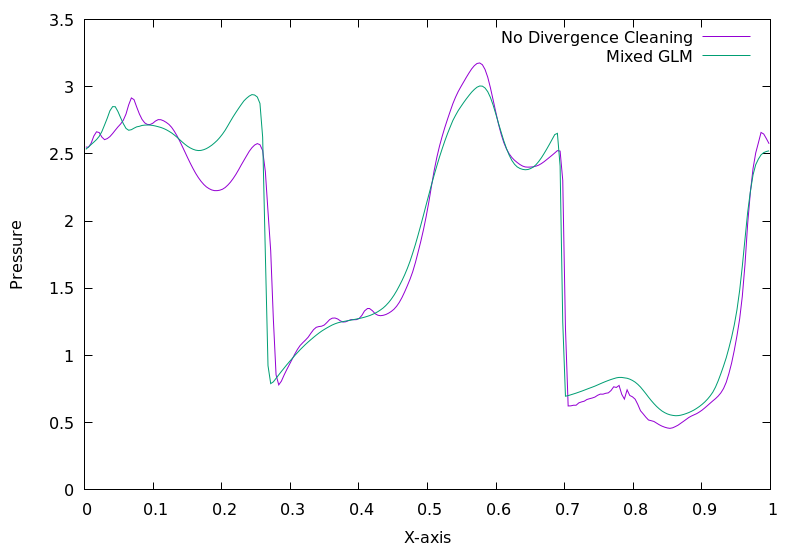
\includegraphics[width=\textwidth]{Oline.png}
\end{minipage}
\begin{minipage}{0.4\textwidth}
  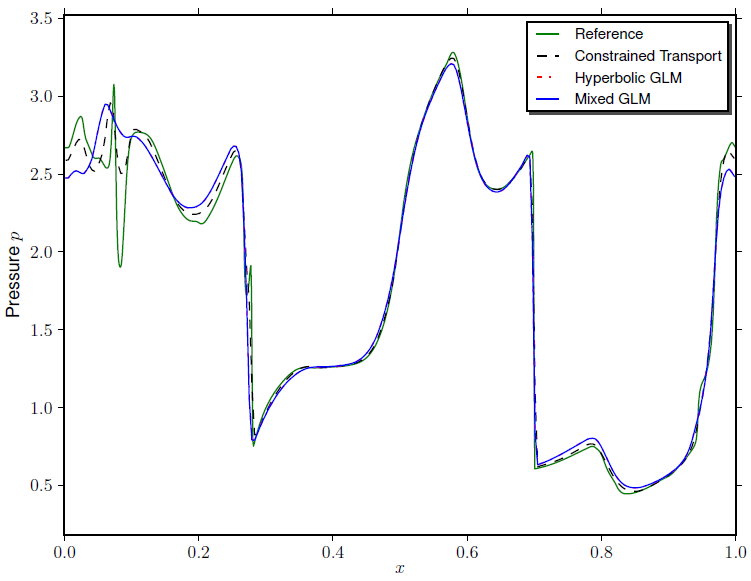
\includegraphics[width=\textwidth]{Oline_vides.png}
\end{minipage}
    \caption[OrszagTang lineout]{Horizontal lineout at $y=0.3125$ showing the gas pressure $p$ in the Orszag-Tang system at $t=0.5$. Our result (left) and Vides \textit{et al.} \cite{vides2013divergence} (right)}
    \label{fig:enter-label}
\end{figure}
\section{Shock Diffraction over Wedge}
We test a two-dimensional case where a shock with Mach number M=1.3 passes over a wedge. This test mainly validates rigid body geometries, especially for wedges and triangles geometries. The configuration is shown in Figure \ref{fig:shockwedgecon}. This shock wave satisfies the normal shock equations \cite{hernandez2018explicit} with M=1.3,   
\begin{equation*}
    \rho_s=\rho_0\frac{(\gamma+1)M^2}{2+(\gamma-1)M^2},\quad p_s=p_0\left[\frac{2\gamma M^2-(\gamma-1)}{\gamma+1}\right],\quad v_{x\_s}=\sqrt{\frac{(\rho_s-\rho_0)(p_s-p_0)}{\rho_s\rho_0}}.
\end{equation*}
We take the atmosphere as the ambient environment. A reference state is used for $\rho_{ref}=1kg/m^3$, $p_{ref}=100000Pa$, $x_{ref}=0.01m$, $v_{ref}=\sqrt{(\gamma p_{ref})/\rho_{ref}}$, $T_{ref}=x_{ref}/v_{ref}$.
Hence, a non-dimensional initial data is $p_0=1.01325$ and $\rho_0=1.225$.
The initial data is given by Table \ref{tab:shockwedge}.
\begin{table}[H]
\centering
\caption{Initial data for shock M=1.3.}
\begin{tabular}{|c|c|c|c|c|}
\hline
State & $\rho$ & $v_x$ & $v_y$ & $p$ \\
\hline
State 1 & $\rho_0$ & 0.0 & 0.0 & $p_0$\\
\hline
State 2 & $\rho_s$ & $v_{x\_s}$ & 0.0 & $p_s$\\
\hline
\end{tabular}
\label{tab:shockwedge}
\end{table}
When discontinuity for shock is set, two acoustic waves are also hidden in it. The acoustic waves affect the shock capturing. This is a well known error that arises from setting up a shock artificially \cite{LeVeque1998,Glaz1985,Hillier1995}. In our numerical simulations, we employed a methodical simplification to isolate the shockwave's effects artificially by refining the regions posterior to the shockwave by setting up the variables just as right behind the shock. This approach was implemented to ensure that the simulations focused exclusively on the propagation and characteristics of the shockwave, minimizing the influence of subsequent disturbances or secondary waves. A resolution of computational domain is $1840\times912$. The results are shown in Figure \ref{fig:shockwedge} and \ref{fig:shockwedge_con} where the figures on the left are taken from \cite{sivier1992vorticity} and correspond to an experiment done by Schardin \cite{schardin1966stossrohre}. In the simulation, oscillations are observed around the sharp angles of the wedge. These perturbations are likely attributable to the numerical challenges associated with modeling sharp geometries. Sharp corners often induce high gradient regions in the flow field, which can lead to numerical instabilities or discrepancies due to insufficient resolution or the inherent limitations of the numerical scheme employed. Enhanced mesh refinement or the implementation of more sophisticated numerical techniques may be required to accurately capture the flow dynamics in these regions.
\begin{figure}
    \centering
    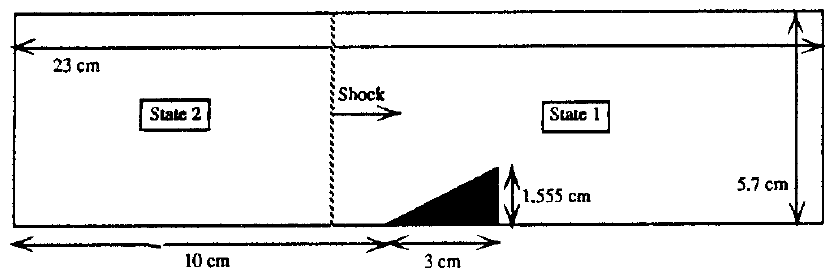
\includegraphics[width=0.9\linewidth]{shockWedgeCon.png}
    \caption[Configuration of Shock Wave and Wedge]{The computational domain configuration in the test of shock wave over a wedge. This plot is adopted from \cite{sivier1992vorticity}.}
    \label{fig:shockwedgecon}
\end{figure}

\begin{figure}
    \centering

\begin{minipage}{0.49\textwidth}
  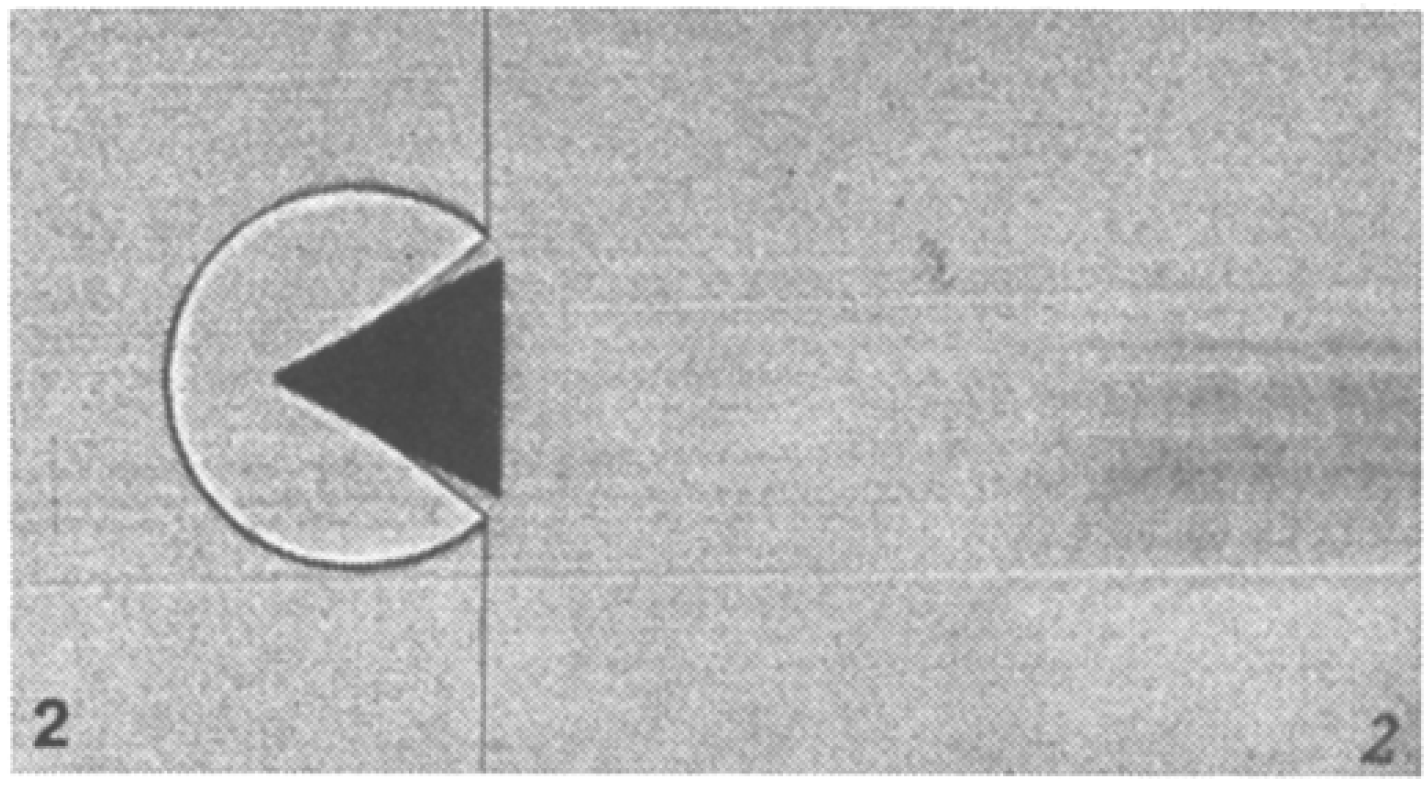
\includegraphics[width=\textwidth]{ShWe1.png}
\end{minipage}
\begin{minipage}{0.49\textwidth}
  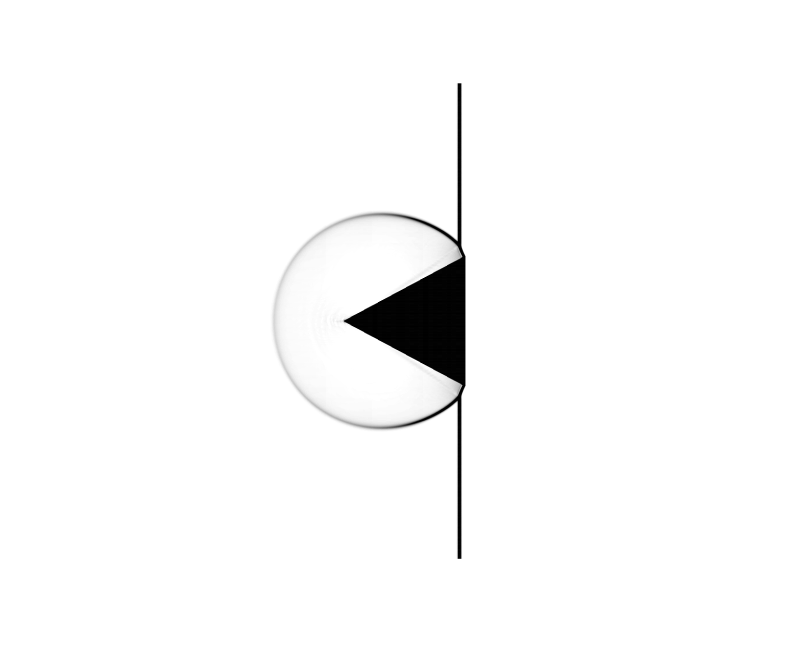
\includegraphics[width=\textwidth]{shock_wedge_2x_270.png}
\end{minipage}
\vspace{-10mm}

\begin{minipage}{0.49\textwidth}
  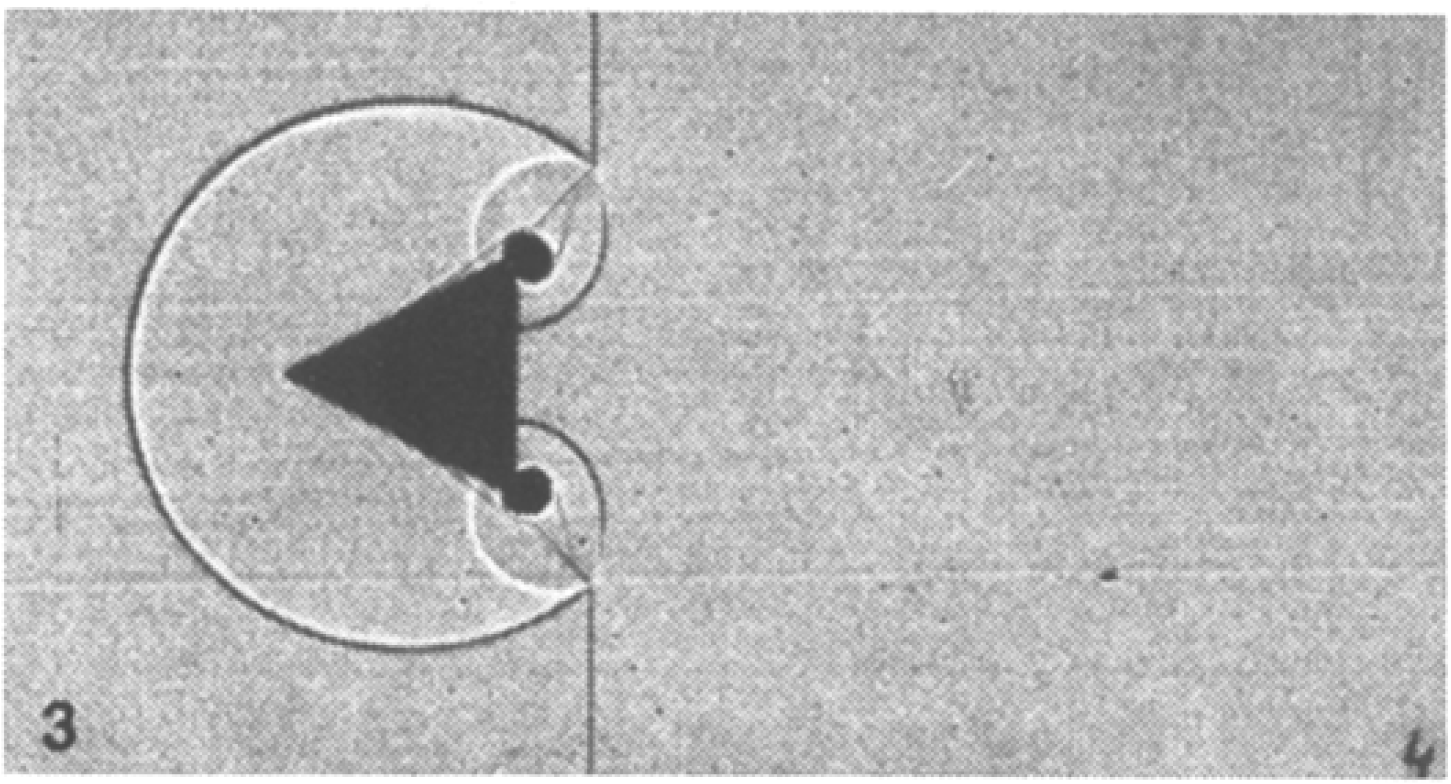
\includegraphics[width=\textwidth]{ShWe2.png}
\end{minipage}
\begin{minipage}{0.49\textwidth}
  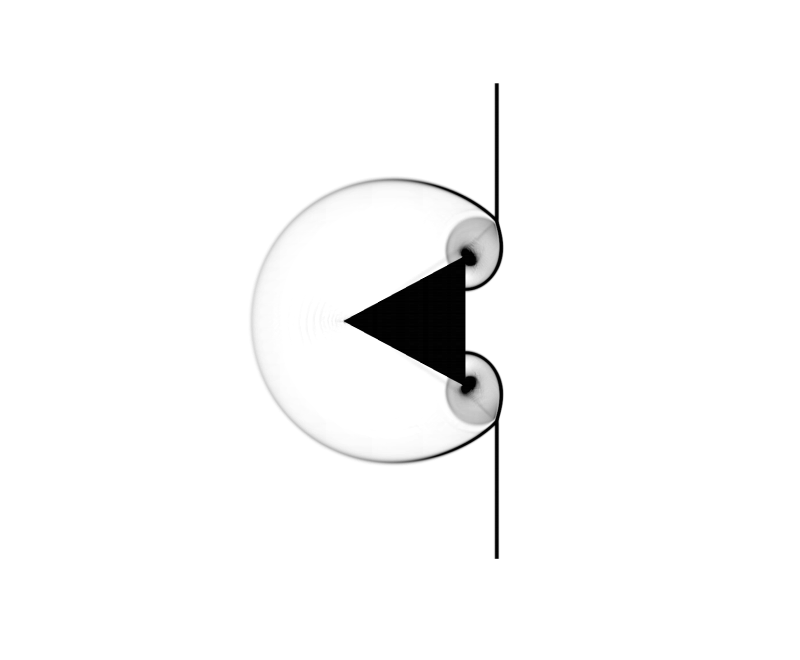
\includegraphics[width=\textwidth]{shock_wedge_2x_340.png}
\end{minipage}
\vspace{-10mm}

\begin{minipage}{0.49\textwidth}
  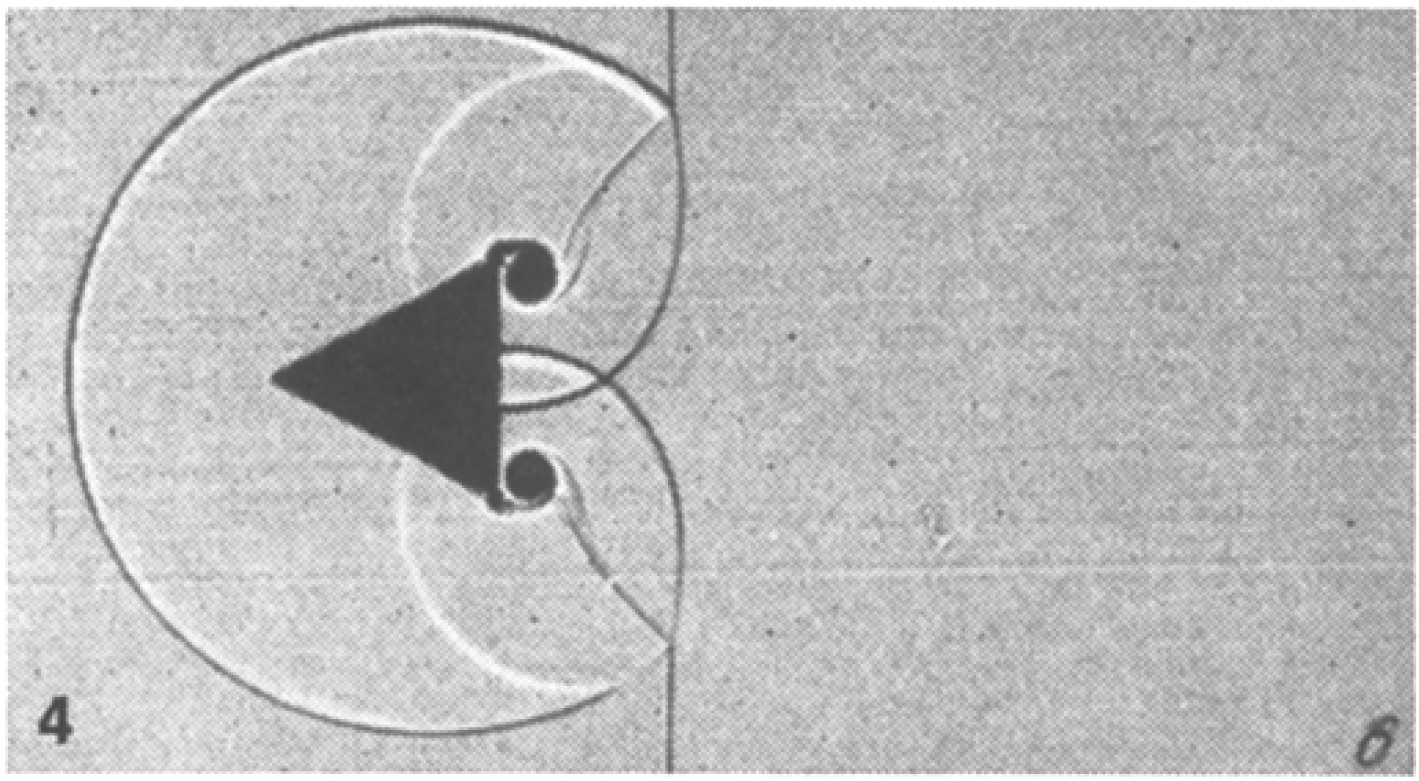
\includegraphics[width=\textwidth]{ShWe3.png}
\end{minipage}
\begin{minipage}{0.49\textwidth}
  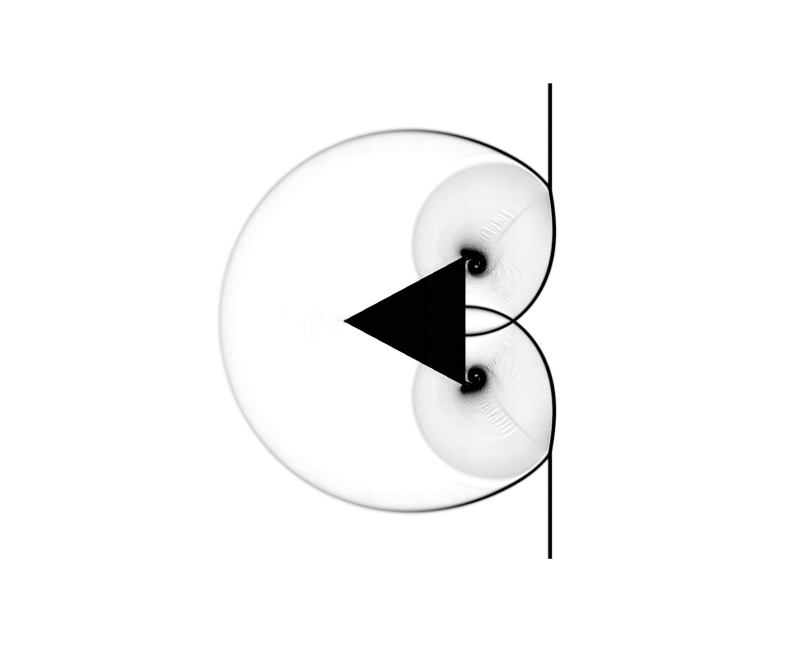
\includegraphics[width=\textwidth]{shock_wedge_2x_440.png}
\end{minipage}
\vspace{-10mm}

\begin{minipage}{0.49\textwidth}
  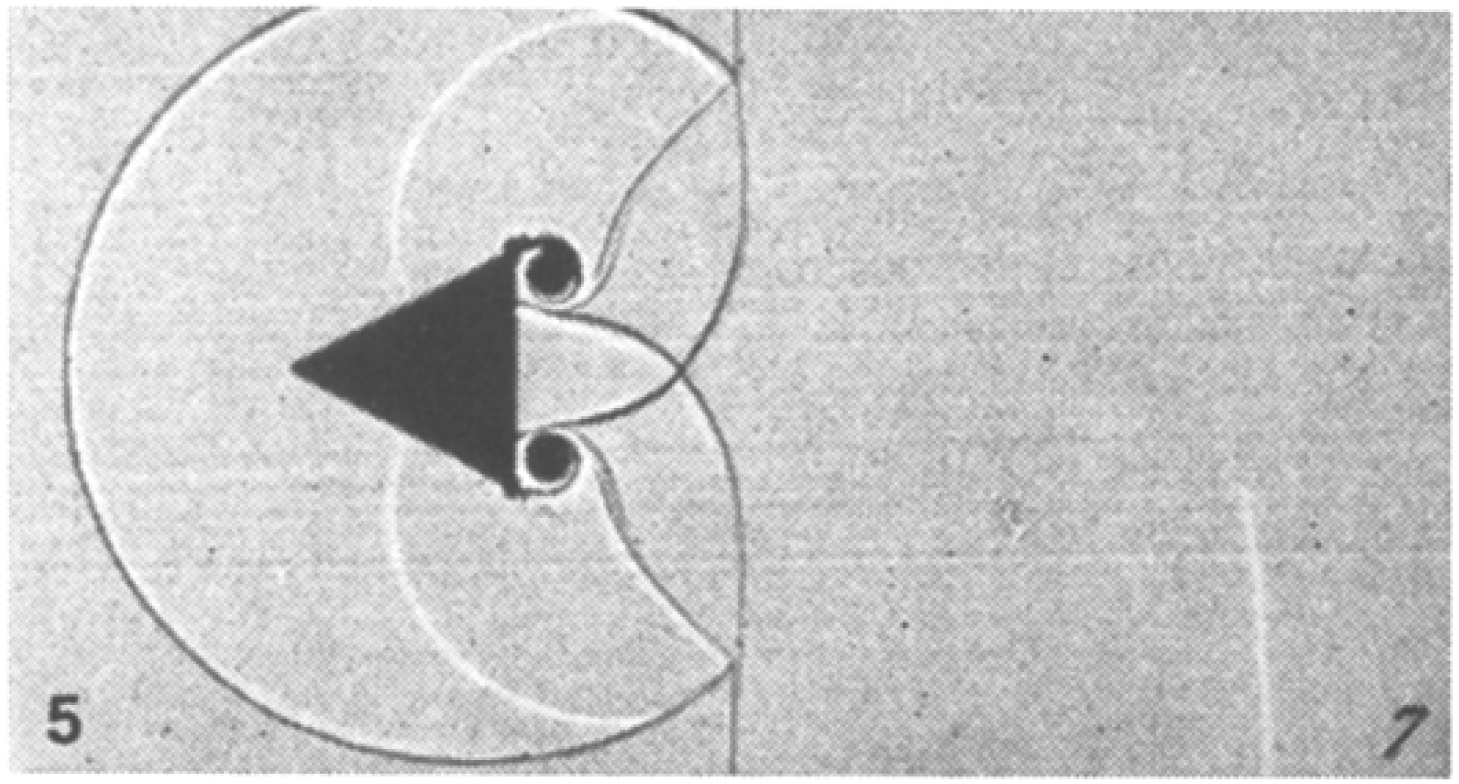
\includegraphics[width=\textwidth]{ShWe4.png}
\end{minipage}
\begin{minipage}{0.49\textwidth}
  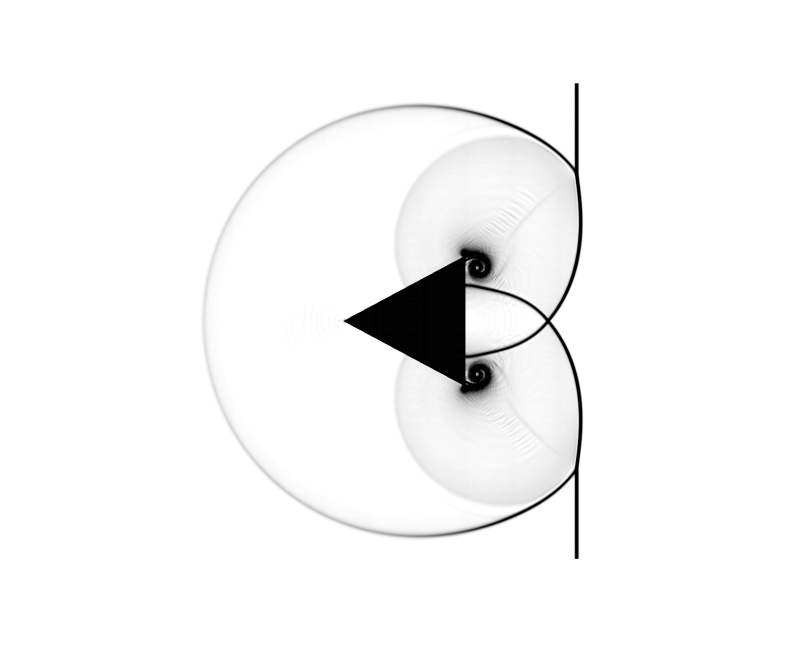
\includegraphics[width=\textwidth]{shock_wedge_2x_490.png}
\end{minipage}

    \caption[Shock diffraction over wedge]{Schlieren plots for Shock M=1.3 diffraction over wedge. The right-hand-side shows the result from simulation. Plots on the left are taken from study \cite{sivier1992vorticity} corresponding to the experiment done by Schardin \cite{schardin1966stossrohre}.}
    \label{fig:shockwedge}
\end{figure}

\begin{figure}

\begin{minipage}{0.49\textwidth}
  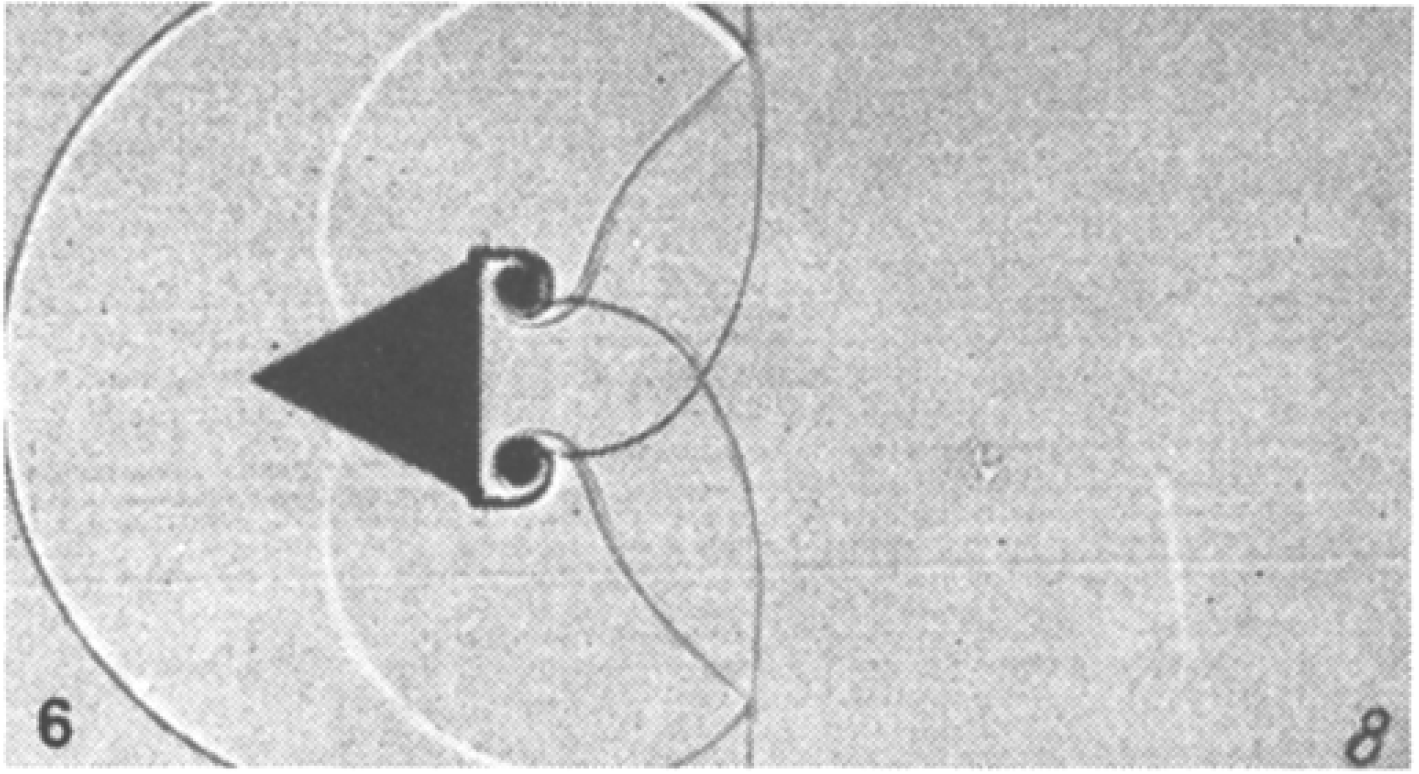
\includegraphics[width=\textwidth]{ShWe5.png}
\end{minipage}
\begin{minipage}{0.49\textwidth}
  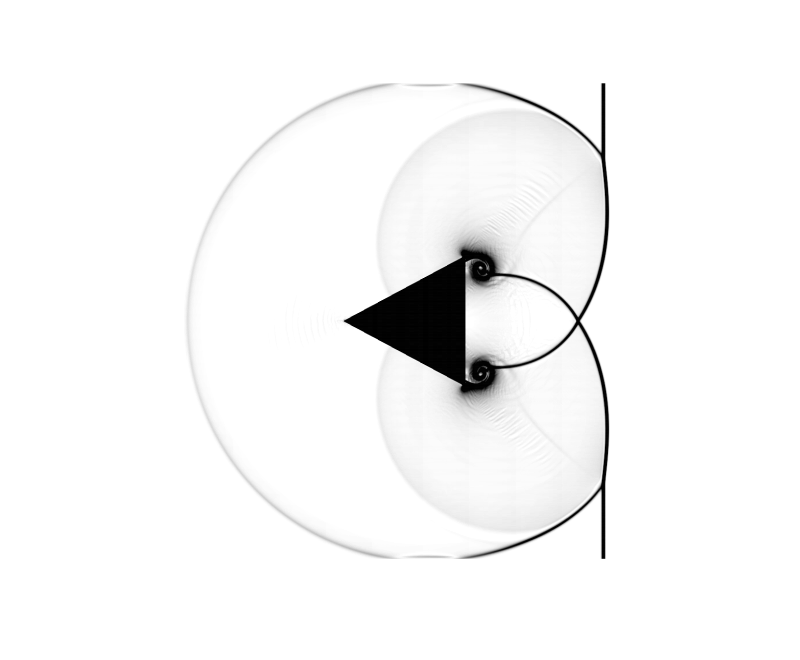
\includegraphics[width=\textwidth]{shock_wedge_2x_540.png}
\end{minipage}
\vspace{-10mm}

\begin{minipage}{0.49\textwidth}
  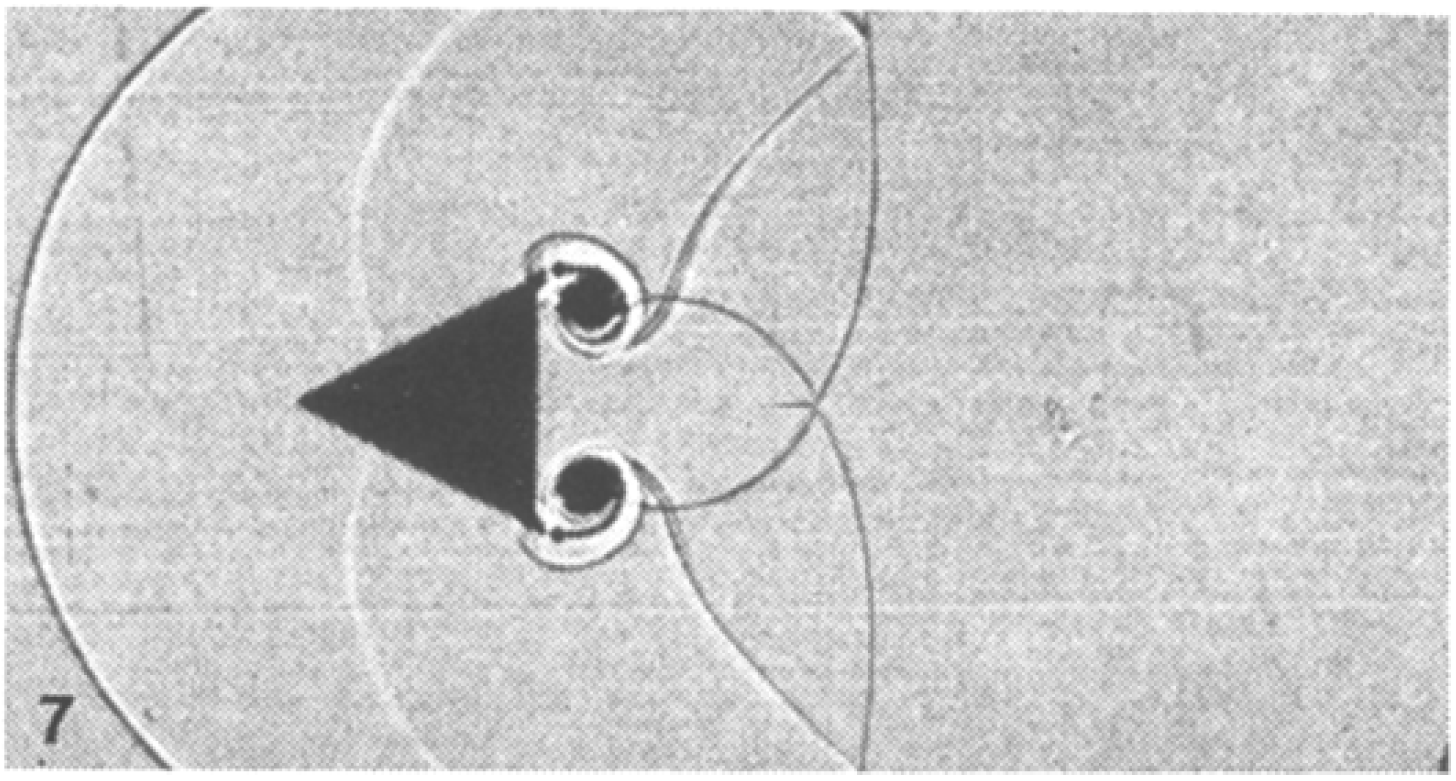
\includegraphics[width=\textwidth]{ShWe6.png}
\end{minipage}
\begin{minipage}{0.49\textwidth}
  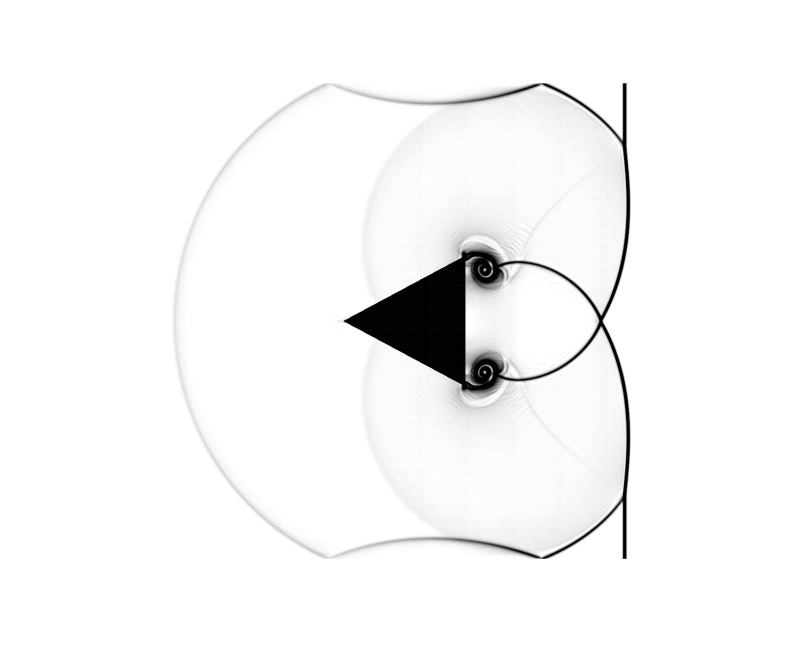
\includegraphics[width=\textwidth]{shock_wedge_2x_580.png}
\end{minipage}
\vspace{-10mm}

\begin{minipage}{0.49\textwidth}
  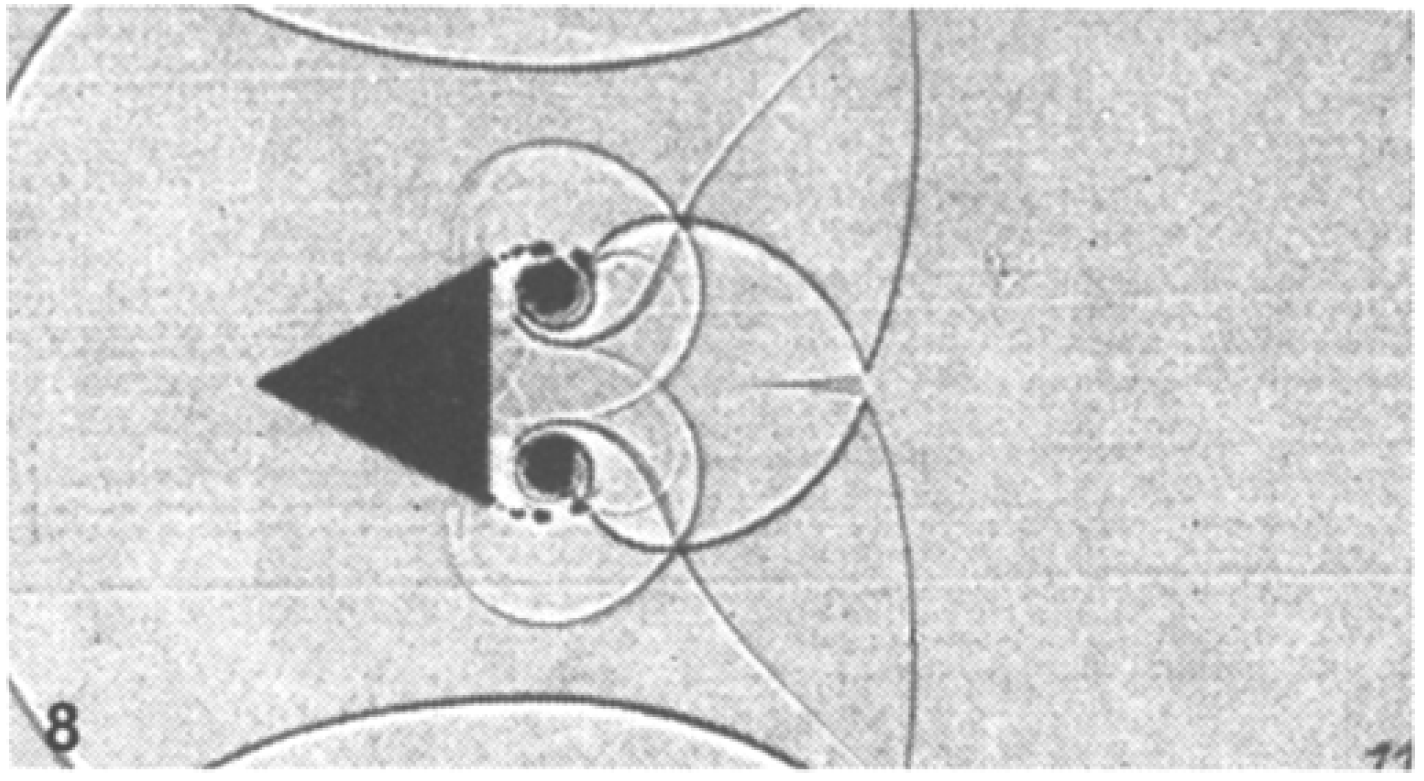
\includegraphics[width=\textwidth]{ShWe7.png}
\end{minipage}
\begin{minipage}{0.49\textwidth}
  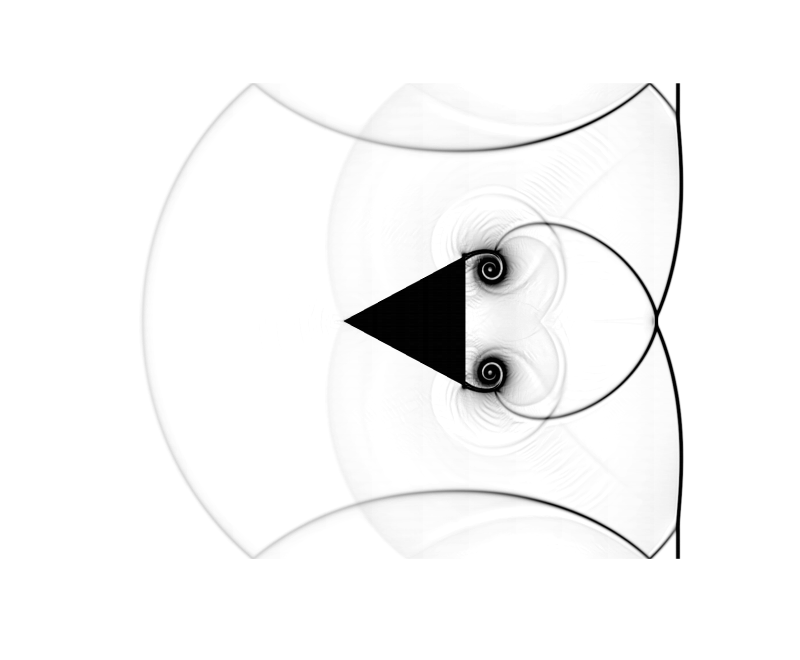
\includegraphics[width=\textwidth]{shock_wedge_2x_680.png}
\end{minipage}

\caption[Shock diffraction over wedge continuing]{Continue plots of Figure \ref{fig:shockwedge}}
    \label{fig:shockwedge_con}

\end{figure}

\section{Shock Diffraction over Cylinder}
A similar two-dimensional case is tested for cylinder with shock M=2.81, using the same normal shock equations and ambient environment, with the same reference states and non-dimensional initial values $\rho_0=1.225$ and $p_0=1.01325$. This test validates circle geometries for rigid bodies. In this test, a similar artificial shock is used. The computational domain is $[0,4]\times[-2,2]$ with $800\times800$ resolution. A circle representing a planar cylinder is set at the center $(2,0)$ with a radius of 0.5. The result is demonstrated in Figure \ref{fig:ShockCy}. The left density image is adopted from \cite{bryson1961diffraction}.

\begin{figure}[htbp]
\centering
\begin{minipage}{0.25\textwidth}
  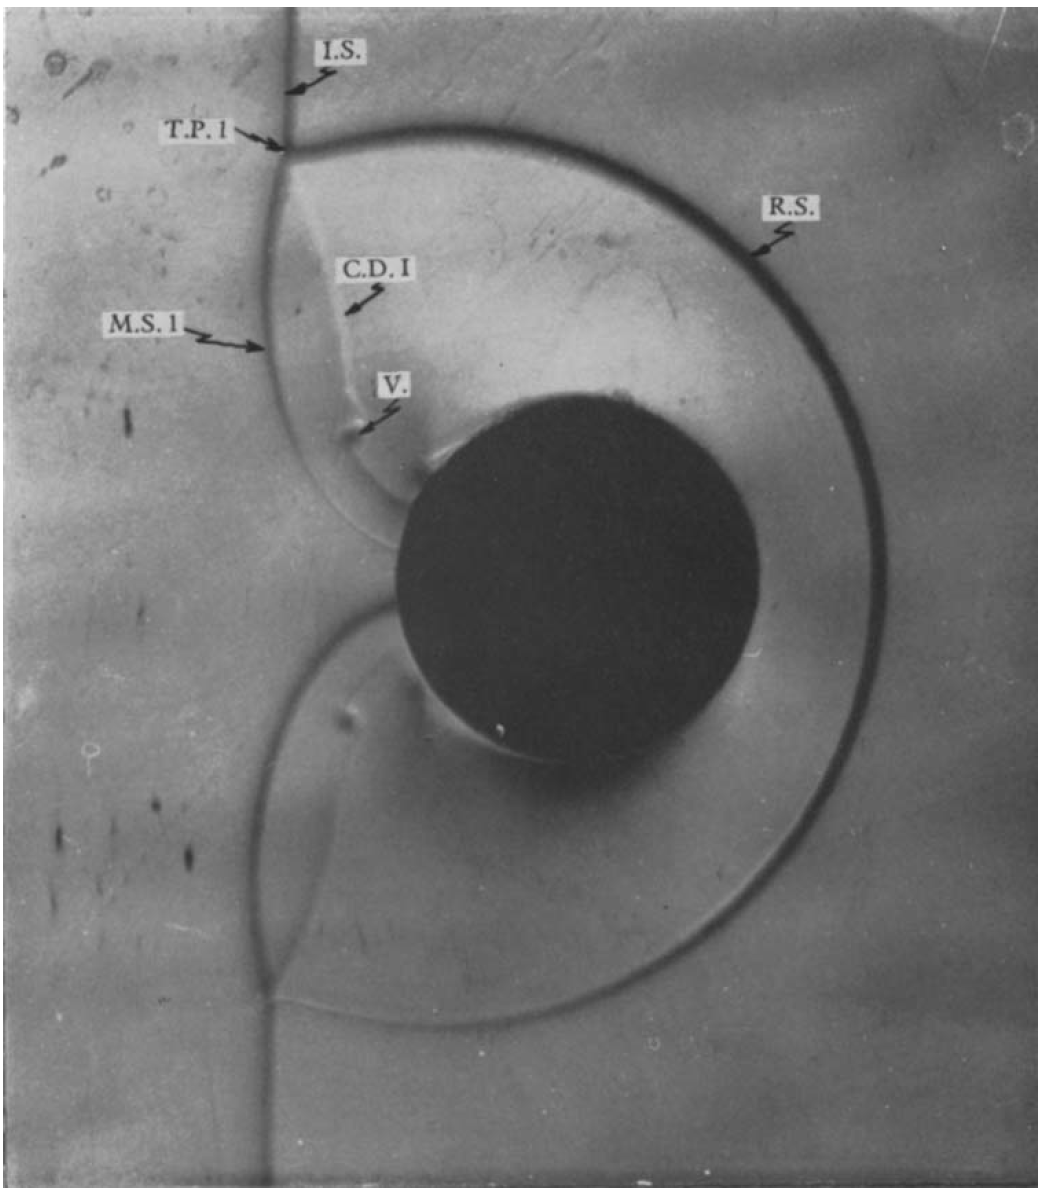
\includegraphics[width=\textwidth]{ShCy.png}
\end{minipage}
\begin{minipage}{0.45\textwidth}
  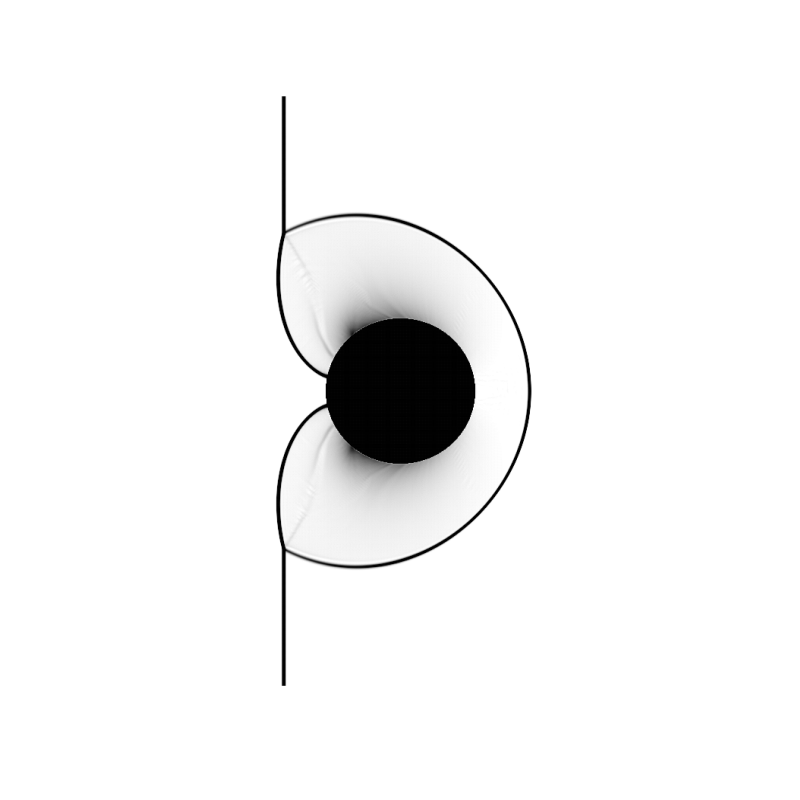
\includegraphics[width=\textwidth]{shock_cylinder_95.png}
\end{minipage}
\caption[Shock diffraction over cylinder]{Schlieren plots for Shock M=2.81 diffraction over a cylinder. The right-hand side shows the result from simulation compared with the image on the left demonstrating the corresponding experiment done by Bryson \cite{bryson1961diffraction}.}
\label{fig:ShockCy}
\end{figure}

\section{Tests in Rotated Rigid Body}
\subsection{Rotated Sod Test}
On the fixed rigid body, we apply a reflective boundary condition, where no-penetration condition and slip condition are used for normal and tangential velocities, respectively. A one-dimensional test is applied to validate the performance of these boundary conditions under the Euler system. 
\begin{figure}[htbp!]
    \centering
    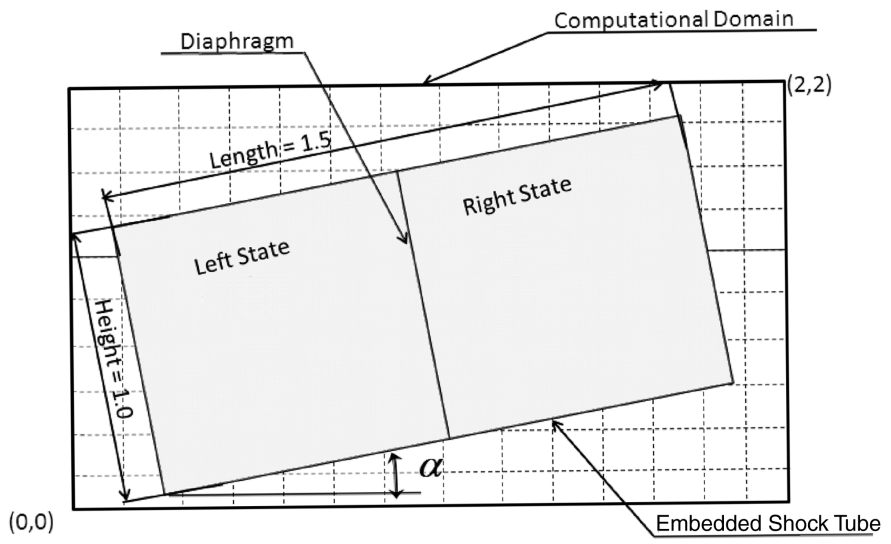
\includegraphics[width=0.5\linewidth]{tube.png}
    \caption[Rotated Tube]{A demonstration of the computational domain and the fixed tube in it. The tube is centered at $(1,1)$ and rotated by an angle $\alpha$. Our tests are mainly conducted within this tube. This plot is adopted from Sambasvian \textit{et al.} \cite{sambasivan2009ghost}.}
    \label{fig:tube}
\end{figure}
As shown in Figure \ref{fig:tube}, we use a computational area of $[0,2]\times[0,2]$ with a resolution $300\times300$, where a rectangle tube is set in this domain with a length of 1.5 and a width of 1.0. The tube is rotated at different angles $\alpha=30^\circ$, $\alpha=45^\circ$, $\alpha=60^\circ$ for throughout testing. The computational test we use is a variant of the Sod test from Toro \textit{et al.} \cite{toro2013riemann}, where the initial states are given in table \ref{tab:sod}.
\begin{table}[H]
\centering
\caption[Sod test]{Initial states for Sod test.}
\begin{tabular}{|c|c|c|c|c|}
\hline
State & $\rho$ & $p$ & $v_x$ & $v_y$ \\
\hline
Left state & 1.0 & 1.0 & 0.0 & 0.0 \\
\hline
Right state & 0.125 & 0.1 & 0.0 & 0.0 \\
\hline
\end{tabular}
\label{tab:sod}
\end{table}
The discontinuity is set in the middle length of the tube. The simulation is carried out to $T=0.25$. We lineout the results in the middle width.  Their densities are demonstrated in lineout Figure \ref{fig:rotateSod} along with the exact solutions and heat Figure \ref{fig:rotateSod_heat}. The results show good agreement with the exact solutions.


  \begin{figure}
      \centering
      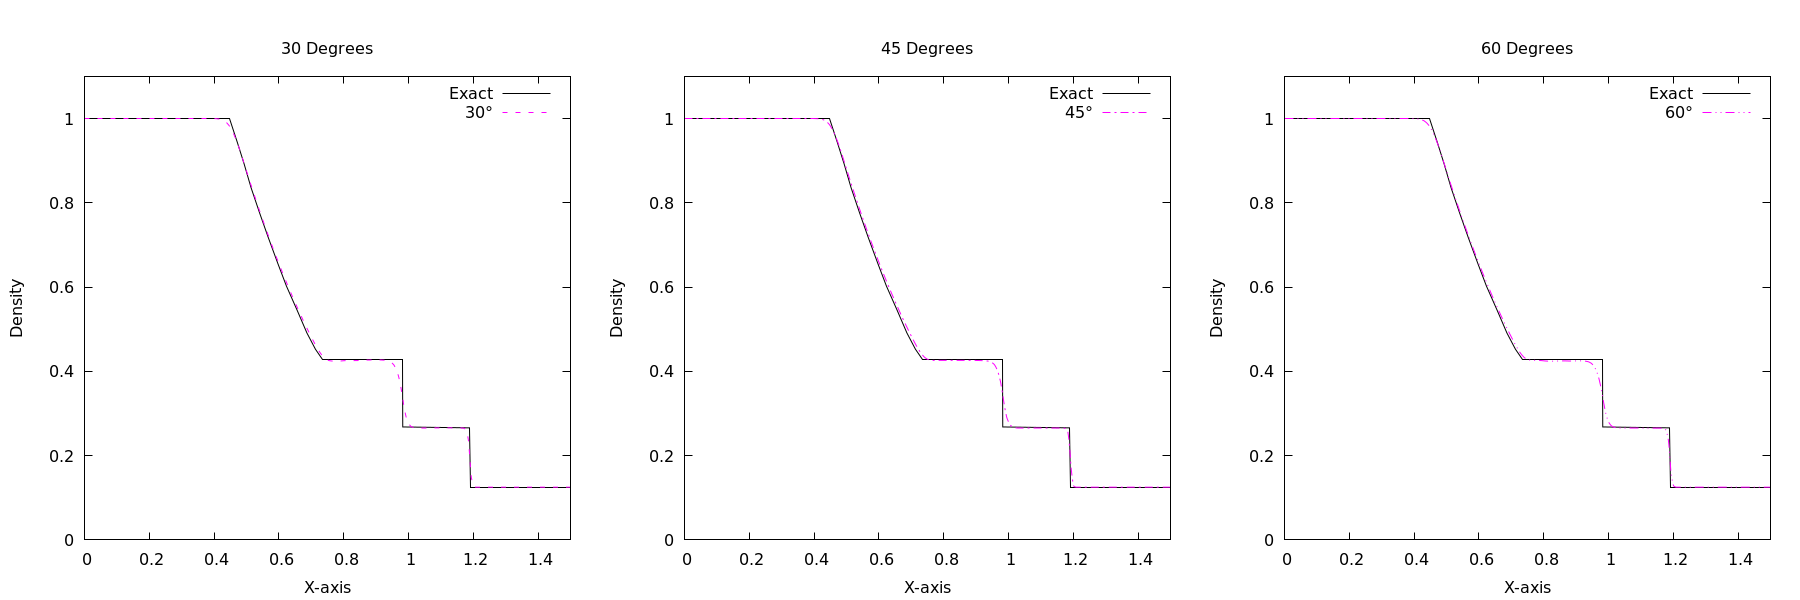
\includegraphics[width=1\linewidth]{rotateSod.png}
      \caption[Lineout for rotated Sod test]{The results of Sod test in a rotated tube with exact solutions. The rotated angles are $\alpha=30^\circ$ (left), $\alpha=45^\circ$ (middle), $\alpha=60^\circ$ (right). Results agree with the exact solutions.}
      \label{fig:rotateSod}
  \end{figure}
  \begin{figure}
      \centering
      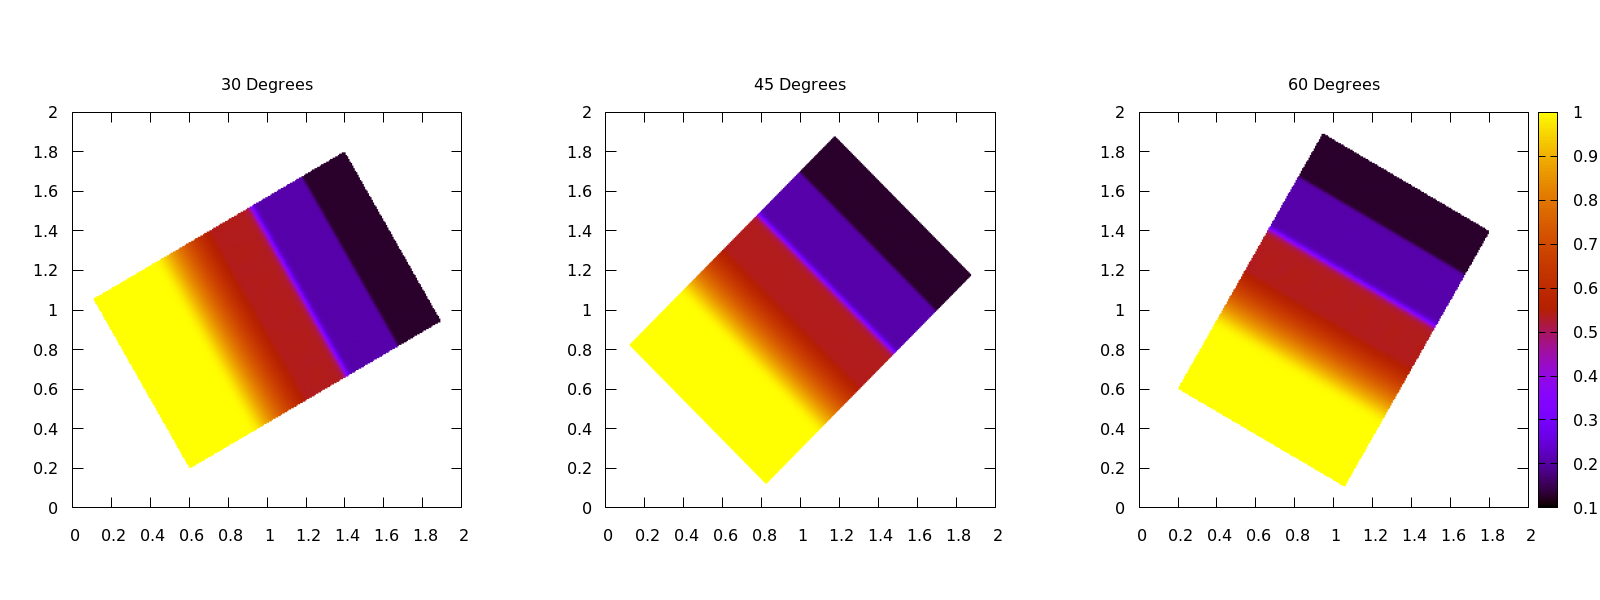
\includegraphics[width=1\linewidth]{rotateSod_heat.png}
      \caption[Heat plot for rotated Sod test]{A heat plot for rotated Sod test showing the tests at different angles.}
      \label{fig:rotateSod_heat}
  \end{figure}
  
\subsection{Rotated Brio-Wu Test}
  The rigid body is regarded as a perfect conductor in validation. A similar 'no-penetration' condition for the normal magnetic field and 'slip' condition for tangential magnetic field are applied. We use the Brio-Wu test \cite{brio1988upwind} to validate these conditions. A similar shock tube is set as shown in Figure \ref{fig:tube}. The Brio-Wu test have a similar initial data to the Sod test but with a non-zero magnetic field and $\gamma=2.0$. Compared with the original test, we adjust the magnetic variables to fit them in the tube. The states for this test are given in Table \ref{tab:Brio}.
  \begin{table}[H]
\centering
\caption[Rotated Brio-Wu test]{Initial states for the rotated Brio-Wu test. $\alpha$ is the rotation angle.}
\begin{tabular}{|c|c|c|c|c|c|c|c|c|}
\hline
State & $\rho$ & $p$ & $v_x$ & $v_y$ & $v_z$ & $B_x$ & $B_y$ & $B_z$ \\
\hline
Left state & 1.0 & 1.0 & 0.0 & 0.0 & 0.0 & $0.75*cos(\alpha)$ & $0.75*sin(\alpha)$ & 1.0 \\
\hline
Right state & 0.125 & 0.1 & 0.0 & 0.0 & 0.0 & $0.75*cos(\alpha)$ & $0.75*sin(\alpha)$ & -1.0\\
\hline
\end{tabular}
\label{tab:Brio}
\end{table}
  A perfect conducting wall condition is applied around the boundary of this tube. We set the initial magnetic field with same normal component as in Table \ref{tab:Brio} with Dirichlet conditions. We reflect the normal magnetic changes on boundary for a 'no-penetration' condition. Such boundary condition stabilize the magnetic field in the shock tube. The simulation is carried out to $T=0.1$. The results are shown in lineout Figure \ref{fig:rotateBrioWu} and heat Figure \ref{fig:rotateBrioWu_heat}. They are similar to the exact solution, which validate the perfect conducing condition we applied. 
  

 \begin{figure}
      \centering
      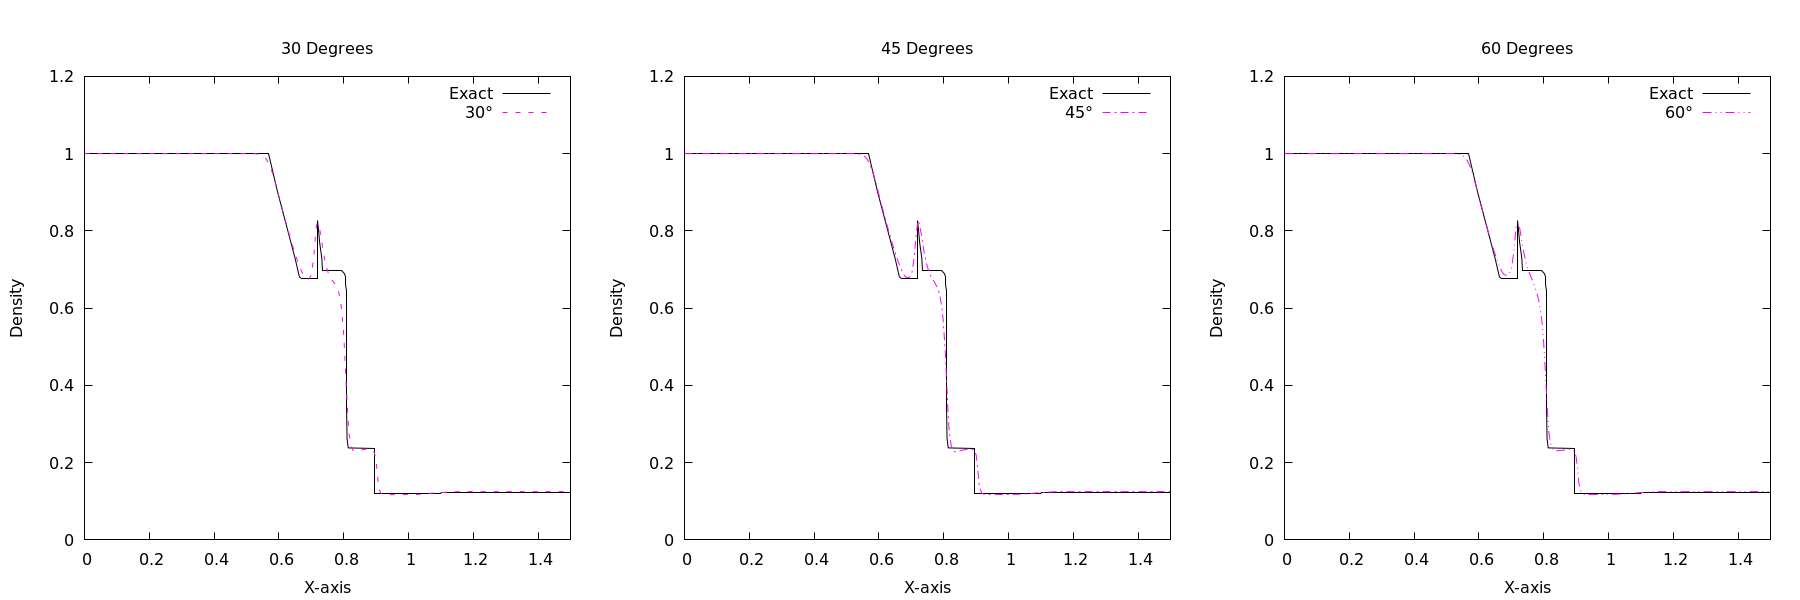
\includegraphics[width=1\linewidth]{rotateBrioWu.png}
      \caption[Lineout for rotated Brio-Wu]{The results of the rotated Brio-Wu test with exact solutions. The results are slightly different from exact solution because of the resolution, but they still validate the perfect conductor condition.}
      \label{fig:rotateBrioWu}
  \end{figure}
  \begin{figure}
      \centering
      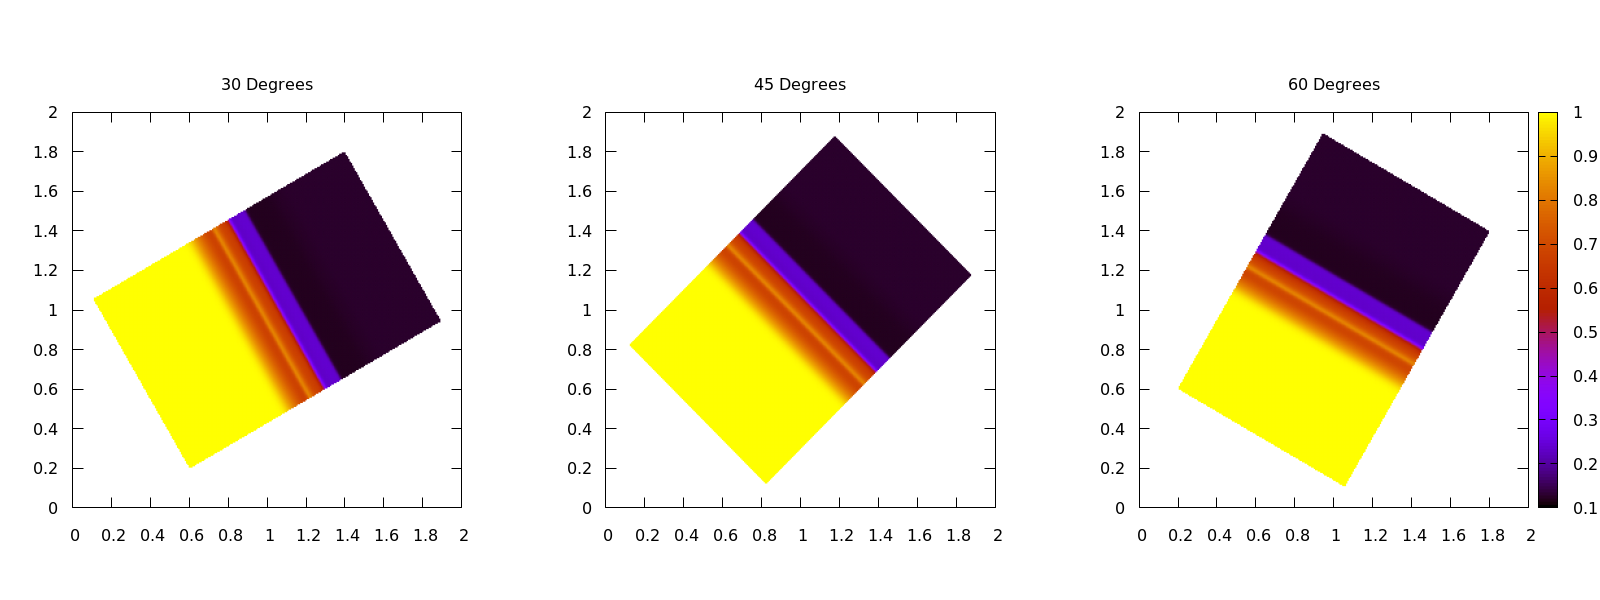
\includegraphics[width=1\linewidth]{rotateBrioWu_heat.png}
      \caption[Heat plot for rotated Brio-Wu test]{A heat plot for rotated Brio-Wu test, showing tests at different angles.}
      \label{fig:rotateBrioWu_heat}
  \end{figure}

  

%!TEX root = ../thesis.tex
%*******************************************************************************
%*********************************** First Chapter *****************************
%*******************************************************************************

\chapter{Summary and Future Work} % Title of the First Chapter

\ifpdf
\graphicspath{{Chapter5/Figs/Raster/}{Chapter5/Figs/PDF/}{Chapter5/Figs/}}
\else
\graphicspath{{Chapter5/Figs/Vector/}{Chapter5/Figs/}}
\fi

\label{chapter 5}

This thesis presented a comprehensive overview of the theoretical foundations and numerical techniques required for simulating ideal magnetohydrodynamic (MHD) phenomena in tokamak devices. The primary objective was to introduce the methodologies and validate their effectiveness through a series of computational experiments.

In Chapter 1, we discussed the significance of nuclear fusion and the critical role of controlled fusion processes, particularly within tokamak reactors. We emphasized the need for precise computational models to aid in the design and optimization of these fusion devices. Chapter 2 delved into the theoretical background, covering the essential ideal MHD equations, various divergence cleaning methods, and the boundary conditions necessary for accurate plasma simulations in tokamaks. We also explored the numerical strategies for handling complex geometries and maintaining the stability of the magnetic field. Chapter 3 outlined the numerical schemes implemented in this study, such as the MHD-HLLC solver and the MUSCL-Hancock method, to achieve second-order accuracy. We described the application of a mixed hyperbolic/parabolic GLM divergence cleaning method to ensure a divergence-free magnetic field. Additionally, we detailed the use of the level set method and reflective boundary conditions for defining and managing rigid body boundaries. Chapter 4 validated the proposed methods through several benchmark tests. The Orszag-Tang test was employed to verify the accuracy of the MHD solver and divergence cleaning techniques, showing good alignment with established results. The shock diffraction tests over wedges and cylinders assessed the handling of rigid body geometries, while the rotated Sod and Brio-Wu tests validated the boundary conditions for both fixed and rotating rigid bodies. These tests confirmed the robustness and reliability of the implemented numerical methods.

While the current study has successfully introduced and validated the theoretical and numerical foundations for ideal MHD simulations within rigid bodies geometries, we are apply these onto more complex cases. We conduct these tests under a perfect conducting wall boundary condition. We may try to extend our results into a resistive wall conditions.

\newpage
\thispagestyle{empty}
\begin{center}
	\vspace*{\fill}
	\Huge\textbf{Report 2}
	\vspace*{\fill}
\end{center}

%!TEX root = ../thesis.tex
%*******************************************************************************
%*********************************** First Chapter *****************************
%*******************************************************************************

\chapter{Resistive Wall Extension} % Title of the First Chapter

\ifpdf
\graphicspath{{Chapter6/Figs/Raster/}{Chapter6/Figs/PDF/}{Chapter6/Figs/}}
\else
\graphicspath{{Chapter6/Figs/Vector/}{Chapter6/Figs/}}
\fi

\label{chapter 6}

In the earlier report 1, we introduced the ideal MHD model employed in our simulations, along with theoretical considerations related to boundary conditions, solvers, and divergence cleaning methods. These techniques were rigorously validated through a series of tests, including the Orszag-Tang test, shock diffraction, and the Brio-Wu test within a rotated, perfectly conducting rigid body.

In this report, we advance the study by exploring the effects of wall resistivity. Specifically, we extend our previous work by replacing the assumption of a perfectly conducting wall with that of a resistive wall, aiming to provide a more realistic simulation of tokamak conditions.

\section{Tokamak Wall Structure}
\label{section6.1}
Tokamaks are advanced devices for achieving controlled nuclear fusion, requiring carefully designed walls to maintain plasma stability. The walls in these devices must provide a magnetic field stabilization, thermal insulation, and radiation shielding \cite{wesson2011tokamaks}. The wall structure is shown in Figure \ref{fig:wallstructure}. A "double-walled" structure is formed by the first wall and the vessel wall, with functional layers in between.  

\begin{figure}[htbp]
	\centering
	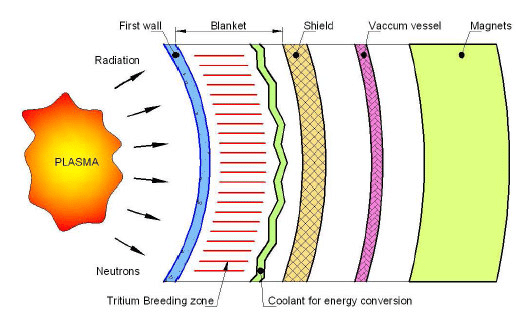
\includegraphics[width=0.7\linewidth]{Wall-Structure.png}
	\caption[Wall Structure for Tokamaks]{Wall structure for tokamaks. The "double-walled" structure in tokamaks often means the first wall and the vessel wall, along with layers between them.}
	\label{fig:wallstructure}
\end{figure}

At the heart of a working tokamak, the fusion plasma must reach temperatures of at least 100 million degrees Celsius. The first wall, as the innermost layer directly exposed to the plasma, must withstand extreme temperatures and high-energy particle bombardment \cite{abdou2015blanket}. To handle these conditions, materials such as beryllium, graphite, and tungsten are commonly employed \cite{wesson2011tokamaks,federici2001plasma,wilson1990beryllium,philipps2011tungsten}. Beryllium is valued for its low atomic number and high thermal conductivity, minimizing plasma contamination \cite{federici2001plasma,wilson1990beryllium}. Graphite offers excellent thermal shock resistance and mechanical stability at high temperatures \cite{federici2001plasma,wilson1990beryllium,philipps2011tungsten}. Tungsten, with its exceptionally high melting point and low sputtering yield, is often used in the divertor region \cite{wesson2011tokamaks,federici2001plasma,wilson1990beryllium,philipps2011tungsten}. These materials ensure that the plasma-wall interface effectively manages heat and minimizes impurity generation.

The vacuum vessel and its wall form an additional wall surrounding the first wall, typically constructed from stainless steel \cite{wesson2011tokamaks,federici2001plasma,iter_website,abdou2015blanket}. This double-walled structure houses essential systems, such as liquid cooling for thermal regulation, divertors for removing hot particles and protecting the first wall, and blanket modules for tritium breeding and neutron moderation \cite{abdou2015blanket}. The vacuum vessel also provides a vacuum space for better heat insulation and plasma confinement, serving as a safety buffer and accommodating various devices \cite{wesson2011tokamaks}.

The outermost layer of a superconducting tokamak consists of superconducting coils made from niobium-titanium (NbTi) and niobium-tin (Nb3Sn) \cite{wesson2011tokamaks, pong2012worldwide}. When cooled below their critical temperatures, these materials exhibit zero electrical resistance, enabling them to carry large currents for magnetic confinement with minimal energy loss. Maintaining these superconducting magnets at cryogenic temperatures, typically between 4K and 4.4K, requires a cryostat and bath of liquid helium \cite{pong2012worldwide, wesson2011tokamaks}. The cryostat, along with the vacuum space, provides thermal insulation, ensuring the superconducting coils stay at the necessary low temperatures despite their proximity to the hot plasma \cite{doshi2011iter, pong2012worldwide}.

ITER \cite{pong2012worldwide} and EAST \cite{wan2005progress} are among the most well-known tokamaks in the world. ITER is focusing on demonstrating the feasibility of large-scale fusion power, and its design incorporates advanced technologies such as plasma monitoring and tritium breeding blankets to sustain the fusion fuel cycle. Meanwhile, EAST explore more on long-duration plasma control technique \cite{wan2005progress}. ITER applies beryllium on the first wall interface while EAST still use tungsten on first wall. However, recent discussions regarding ITER suggest the potential application of tungsten on the first wall \cite{iter_website}. On both of ITER and EAST, tungsten is applied on divertor. Both of their vacuum vessels are made by stainless steel while ITER's vessel also houses some extra blanket modules designed for tritium breeding and neutron moderation. As for the superconducting coils, ITER use NbTi on poloidal field and Nb3Sn on toroidal field \cite{pong2012worldwide}, cooling by helium bath around 4K. For EAST, both coils of toroidal field and poloidal field take NbTi as primary choice. While there are technical differences between ITER and EAST, both are designed to achieve successful and sustainable fusion, with no expected significant disparities in their outcomes.

\section{Wall Modeling}
As discussed in the Chapter \ref{chapter 2}, the ideal MHD model is an appropriate approximate model for fusion plasma. In temperatures higher than 100 million degrees Celsius, the plasma is fully ionized and can be accurately described as an ideal plasma with no resistivity and viscosity.

The numerical modelling of tokamaks has been the focus of numerous studies in the literature. Some of these works regard the tokamak wall, as perfect conductor. Todd \textit{et al.} focuses on analyzing the stability of plasma configurations in tokamaks using the ideal MHD within perfect conducting walls \cite{todd1979dependence}. Pustovitov \textit{et al.} provides a comprehensive analysis of disruption forces in tokamaks using ideal MHD and perfect conducting wall assumptions, with a particular focus on applications to ITER \cite{pustovitov2017computation}. These conditions have benefits. The perfect conducting wall boundary condition can help stabilize certain MHD. By assuming that the wall is perfectly conducting with no resistivity, it can reflect any magnetic field perturbations as we discussed in the chapter \ref{chapter 2}, effectively providing a stabilizing effect on the plasma. This boundary condition simplifies the mathematical analysis and numerical implementation. These models are valuable for qualitative studies of the interactions between plasma and reactor walls.

In practice, no material exhibits perfect conductivity; even the most advanced superconductors possess inherent limitations. Modeling the wall as a perfect conductor ignores the actual electrical resistivity of materials used in tokamak walls. Most of the materials used on tokamak walls have finite resistivity. Ignoring the resistivities on these materials may lead to neglect on energy dissipation or magnetic field diffusion and the possibility of plasma instability \cite{pustovitov2017computation}. Generally, a perfect conducting condition simplify mathematical analysis but ignore resistive effects \cite{bondeson2003physics}. For more accurate results, modeling the tokamak wall as a perfect conductor is somewhat idealistic.

Modeling the tokamak walls as resistive walls is a more realistic approach. The materials, such as beryllium, graphite, or tungsten on the first wall and stainless steel on the vacuum vessel wall, are better described as resistive materials. Several studies have considered the effects of resistive walls, noting that their resistivities can lead to magnetic field diffusion and impact plasma behavior \cite{chrysanthou2020, ferraro2016multi, becerra2016resistive}. Over time, some magnetic fields may penetrate the wall, a phenomenon known as resistive wall mode (RWM), which may result in plasma instability \cite{clauser2021iter,bondeson2003physics}. Generally, resistive wall is a more realistic boundary condition under the scenario in a tokamak.

The following chapters, starting with chapter \ref{chapter 7}, will explore the theoretical foundations of resistive wall boundary conditions. In chapter \ref{chapter 8}, we will present a series of validation tests to compare the results of resistive wall conditions with those of a perfect conducting wall, demonstrating the impact on plasma behavior, further then apply these validated methods to a simulation within a tokamak-shaped vessel, illustrating the practical implications of our model. The report will conclude in chapter \ref{chapter 10} with a discussion on strategies for improving the accuracy of boundary conditions in future research.

 

 

%!TEX root = ../thesis.tex
%*******************************************************************************
%*********************************** First Chapter *****************************
%*******************************************************************************

\chapter{Theory} 

\ifpdf
\graphicspath{{Chapter7/Figs/Raster/}{Chapter7/Figs/PDF/}{Chapter7/Figs/}}
\else
\graphicspath{{Chapter7/Figs/Vector/}{Chapter7/Figs/}}
\fi

\label{chapter 7}


In the report 1, we discussed the fundamental aspects of the ideal Magnetohydrodynamics (MHD) model used to describe plasma behavior in tokamaks. The ideal MHD framework, characterized by the absence of resistivity and viscosity, provides a simplified yet reasonable model for understanding the core plasma in tokamak. The key solvers of this model, including the MHD-HLLC solver and the MUSCL-Hancock method, were validated through a series of tests in Report 1. A mixed hyperbolic/parabolic Generalized Lagrange Multiplier (GLM) divergence cleaning method is used to maintain the divergence-free nature of the magnetic field. We validate these in the report 1. These methods and techniques are still going to be applied in report 2. In this chapter, we focus our attention on the mathematical theory towards a resistive wall condition.

\section{Resistive Wall Equation}
\label{section7.1}
In section \ref{section2.3}, we discuss some of the necessary mathematical requirements for perfect conducting or insulating wall conditions. More specifically, we expressed a perfect conducting or insulating wall in terms of Dirichlet or Neumann boundary conditions for the magnetic field. However, the resistive wall condition is too complicated to be described as Neumann or Dirichlet conditions. Instead, the equations governing the magnetic field on fixed rigid body are Faraday's Law:
$$
\frac{\partial \mathbf{B}}{\partial t} + \nabla \times \mathbf{E} = 0 ,
$$ 
Ampere's Law:
$$
\frac{1}{c^2}\frac{\partial \mathbf{E}}{\partial t} + \mu_0 \mathbf{J} - \nabla \times \mathbf{B} = 0  
$$
and Ohm's Law:
$$
\eta \mathbf{J} = \mathbf{E} + \mathbf{v} \times \mathbf{B} .
$$

The change in the electric field is much slower than speed of light. $\frac{1}{c^2}\frac{\partial \mathbf{E}}{\partial t}$ can be regarded as small term and be ignored. For a fixed rigid body, $\mathbf{v}=0$. These equations give the magnetic diffusion on rigid body
\begin{equation}
	\frac{\partial \mathbf{B}}{\partial t}+\eta_{w}\nabla\times\nabla\times\mathbf{B}=0
	\label{equ:magneticDiffusion}
\end{equation} 
where $\eta_w$ is the resistivity on wall. Since the identity $\nabla\times\nabla\times\mathbf{B}=\nabla(\nabla\cdot\mathbf{B})-\nabla^2\mathbf{B}$ and  $\nabla\cdot\mathbf{B}=0$, this equation can be further rearranged as 
\begin{equation}
	\eta_{w}\nabla^2\mathbf{B}=\frac{\partial \mathbf{B}}{\partial t}
	\label{equ:magneticDiffusion_rearrange}
\end{equation} 
\section{Stiffness Problem from Diffusion}
We deduced the magnetic diffusion equation \ref{equ:magneticDiffusion} on rigid body. This equation might have a different stable time step compared with the numerical scheme used for the plasma, leading to the occurence of a stiffness problem.

Generally, the stiffness problem arises in numerical simulations when some terms act on much shorter time scales for compared to the rest of the system \cite{wright2020resistive}. To be more specific, some terms may lead to much smaller time steps compared with the rest of the numerical equation to guarantee numerical stability \cite{spijker1996stiffness}. In our case, the magnetic diffusion equation \ref{equ:magneticDiffusion} on rigid body may need to evolve in a much shorter time step than that in plasma. That is how it forms a stiffness problem under the resistive wall condition. In order to maintain numerical stability and effectiveness, addressing the stiffness in the problem may necessitate the use of very small time steps in an explicit method, or alternatively, employing an implicit method. However, this can lead to high computational costs and prolonged computation times, potentially rendering large-scale simulations impractical \cite{spijker1996stiffness,wright2020resistive}. Similar stiffness problem also occur in resistive MHD model \cite{wright2020resistive}, chemical kinetics, control systems and any system with processes occurring at vastly different rates \cite{spijker1996stiffness}.     

\subsection{Evaluating Stiffness}
\label{section7.2.1}
To quantitatively determine the stiffness of a set of numerical equations, particularly differential equations, we need to assess the properties that contribute to stiffness. It has proven difficult to formulate a precise definition of stiffness, but some studies proposed ways to quantitatively evaluate stiffness. Spijker \cite{spijker1996stiffness} use Lipschitz constant, upper bound of absolute value of gradient locally in time and space, to evaluate the stiffness. Thohura \textit{et al.} \cite{thohura2013numerical} use the largest negative eigenvalue of Jacobian matrix of the numerical equation while Chu \textit{et al.} \cite{chu1996evolutionary} just do a sensitivity analysis. 

To some extent, the resistivity that causes magnetic diffusion in a rigid body is quite similar to the resistivity in resistive MHD plasma, except that on the fixed rigid body, there is no velocity. Under most of the definitions above, both of their model stiffness is proportional to resistivities \cite{wright2020resistive}. That is $\textit{stiffness}\propto \eta$. In chapter \ref{chapter 7}, we discussed the materials use in tokamaks devices. Beryllium, graphite, and tungsten are used in first wall and stainless steel is used on vacuum vessel wall. The resistivities for beryllium and tungsten are $4.0 \times 10^{-8} \, \Omega \cdot \text{m}$, $5.6 \times 10^{-8} \, \Omega \cdot \text{m}$. The highly ordered pyrolytic graphite used on tokamaks has lower resistivity than normal graphite, with a resistivity less than or equal to $1 \times 10^{-6} \, \Omega \cdot \text{m}$. That on stainless steel is around  $7 \times 10^{-7} \, \Omega \cdot \text{m}$. Thus, the rigid body resistivity in equation \ref{equ:magneticDiffusion} should have $\eta_w\leq1 \times 10^{-6} \, \Omega \cdot \text{m}$, which implies that our numerical methods need to be capable of handling this range of resistivity values effectively.

\subsection{Approaches for Stiffness}
In numerical simulations, stiffness problems often necessitate specialized approaches to ensure stability and efficiency. Two of the most common strategies are adaptive time stepping and implicit methods. Adaptive time stepping involves adjusting the time step size dynamically to accommodate the varying scales of the problem, which helps to maintain stability without overly restricting the step size. On the other hand, implicit methods are particularly effective for stiff problems as they allow for larger time steps while maintaining stability, albeit at the cost of increased computational complexity. Both approaches are crucial in managing the challenges posed by stiffness in simulations.
\subsubsection*{Adaptive Time Step and Subcycling}
Solving these stiffness problems can be equivalent to numerically solving stiff ordinary differential equations (ODEs). The most straightforward approach is adaptive strategies. Spatially, adaptive mesh refinements are often used to reduce mesh stiffness in areas of interest, with mesh stiffness serving as a criterion for refinement. Offermans \textit{et al.} \cite{offermans2020adaptive} note that p-refinement may lead to local mesh stiffness outside the target area. Temporally, adaptive techniques are commonly applied to solve ODEs. For instance, adaptive stepsize control in Runge-Kutta methods helps avoid the limitations of fixed stepsizes, which can introduce significant round-off errors in Thohura and Rahman \cite{thohura2010comparison}. Similar techniques have been shown to improve efficiency and accuracy in solving stiff initial value problems in Jannelli and Fazio \cite{jannelli2006adaptive}. Subcycling is another direct adaptive method; LeVeque and Yee \cite{LeVeque1998} split the problem into conservation laws and stiff source systems, applying an ODE solver over subdivided time intervals to handle the stiff source term. Kershaw \cite{kershaw1981differencing} also employs subcycling to address diffusion in hydrodynamics. These methods, adaptive stepsize control and subcycling, are flexible, efficient, and accurate across different scales by focusing on local stiffness and controlling round-off error within acceptable limits.

\subsubsection*{Implicit Methods}
Many methods have been developed to tackle stiffness in differential equations, with implicit methods being particularly effective. Implicit methods have a natural advantage in dealing with stiffness problems as they often have A-stability remaining stable with large step size or L-stability ensuring not accumulating errors over time \cite{alamri2022very}. These situations are called unconditional stable. For instance, the Backward Euler Method, as employed by Liu \textit{et al.} \cite{liu2012efficient}, efficiently solves nonlinear dynamic problems in structural engineering, offering unconditional stability for stiff systems. Similar to Backward Euler, Rosenbrock methods is also a implicit single-step method that effectively address stiff ODEs \cite{shampine1982implementation}.

Intermediate-step methods have better accuracy, such as implicit Runge-Kutta (IRK), specially including Gauss-Legendre method, Radau method and Lobatto method. Implicit Runga-Kutta methods are particularly effective in handling stiffness in differential equations with A-stability and L-stability \cite{alamri2022very,franco1997two}. Franco and Gomez \cite{franco1997two} demonstrate the effectiveness of IRK methods in solving stiff equations due to their unconditional stability.

Implicit trapezoidal method is based on the trapezoidal rule for integration known as the simplest multistep method. It averages the function's values at the current and next time steps. Crank-Nicolson method, as special application of these methods, averages function values over time steps as shown by Jorgenson \cite{jorgenson1unconditional}. 
 
Some advanced multistep methods can also be used on dealing with stiff problem. The Adams-Bashforth methods \cite{jorgenson1unconditional} are typical multistep methods. However, they are explicit and not very good at solving stiff equations. Instead, Adams-Moulton methods are implicit and better to solve stiff equations. Among all multistep method, Backward Differentiation Formulas (BDF) are the most famous for their good performance on solving stiff ODE. BDF are implicit and multistep. All of them are A-stable but only some of them are L-stable. They are introduced by Curtiss and Hirschfelder in 1952 \cite{curtiss1952integration} to especially address stiffness in equations. They are the most powerful methods on stiffness problem. 

Although implicit methods are naturally good at solving stiff equations as they have bigger stable time step, they require the solution of large systems of nonlinear equations, often acquired by iterative techniques and matrix operations. A Jacobian matrix needs to be solved during the iteration. This complexity increases rapidly as the problem scale increase. 

\subsubsection*{Addressing Our Stiffness Problem}
In our case, there are several advantages that we must consider. The stiffness problem primarily occurs on the resistive wall. The resistive wall condition, as a boundary condition, is inherently separate from the core ideal MHD model that we evolve. Additionally, the stiffness associated with the resistive wall condition mainly stems from $\eta_w$ in magnetic diffusion equation \ref{equ:magneticDiffusion}, where $\textit{stiffness}\propto \eta_w$. As discussed in the end of section \ref{section7.2.1}, $\eta_w$ is small under a tokamak scenario. Given these, it is not justified to bear the high computational cost of using any implicit method. Therefore, the solution to addressing the stiffness here is clear. We should follow the approach outlined by LeVeque and Yee \cite{leveque1990study}. We separate the condition on the rigid body and update the magnetic diffusion with subdivided subcycles. Practically, we build up a state of rigid body. We evolve the states on the plasma and the rigid body alternately as if the ghost fluid method is applied. This approach allows us to manage the stiffness without incurring high computational costs. Specifically, the subcycling time step on the rigid body follow the CFL condition based on Von Neumann stability analysis on magnetic diffusion with reference to Dumbser \textit{et al.} \cite{dumbser2019divergence}. we use the following as our stable time step for the stiff ODE. This is used as a guide for the number of subcycling steps we take in our split approach.  
$$
\Delta t=CFL\frac{1}{2{{\eta }_{w}}\left( \frac{1}{\Delta {{x}^{2}}}+\frac{1}{\Delta {{y}^{2}}} \right)}
$$  

\section{Boundary Condition for Divergence Cleaning}
In chapter \ref{chapter 3}, we discussed the mixed divergence cleaning we use. When simulating with the involvement of rigid bodies, divergence cleaning becomes very important. Divergence cleaning can address the divergence errors introduced by plasma-wall interactions. While divergence-free conditions may be maintained within the plasma or rigid body, interactions between plasma and the wall can easily create a non-zero divergence, violating the divergence-free condition. Therefore, when a rigid body is present, it is crucial to choose suitable boundary conditions for the divergence cleaning potential. $\psi$ is the potential representing non-zero magnetic divergence and is used to reduce divergence errors. The mixed divergence cleaning approach employs hyperbolic and parabolic terms to dissipate and dampen $\psi$. We aim to avoid the spread of divergence across the boundary during cleaning. Consequently, we apply Neumann boundary conditions, specifically transmissive conditions, to ensure that $\psi$ remains consistent across the boundary, eliminating any corrections between them.

%!TEX root = ../thesis.tex
%*******************************************************************************
%*********************************** First Chapter *****************************
%*******************************************************************************

\chapter{Resistive Wall Simulation}  %Title of the First Chapter

\ifpdf
    \graphicspath{{Chapter8/Figs/Raster/}{Chapter8/Figs/PDF/}{Chapter8/Figs/}}
\else
    \graphicspath{{Chapter8/Figs/Vector/}{Chapter8/Figs/}}
\fi

\label{chapter 8}


%************************************************************************** 
\section{Validation Challenge}
We try to validate the resistive boundary condition we are using. However, in contemporary research, the validation of resistive wall models remains a challenging task. Several factors contribute to this challenge. Firstly, there are no experiments and standard tests cases for resistive wall simulations. In hydrodynamics, there are a lot of visualized experiments like shock diffractions done by Bryson \cite{bryson1961diffraction} and Schardin \cite{schardin1966stossrohre}. In MHD, there are several benchmark tests, such as Brio-Wu and Orszag-Tang rotor problem while most of them are remained numerically. Unlike the well-established scenarios in hydrodynamics, MHD often involve extreme conditions and complex effects \cite{pu2024unified} so that less experiments can be done and used in numerical validations. Among the existing benchmark tests, some, like the Brio-Wu test, are one-dimensional and cannot reflect the effects of a resistive wall, while others are not stable enough to be used for validating resistive walls. Additionally, even for a same test, the diversity in modeling approaches and purposes in different studies make it hard to have a standard result. Some may study the external kink instability and only model locally, like  Ghatak \textit{et al.} \cite{ghatak2007kink}. Some may use a resistive MHD model while we are using a ideal MHD model \cite{becerra2016resistive}. Due to these challenges, establishing a universally accepted validation method for resistive wall models is elusive. 

A cylindrical equilibrium test is employed by Ferraro \textit{et al.} \cite{ferraro2016multi} designed to model the resistive wall mode (RWM) within a simplified straight cylindrical geometry to compare the calculated linear growth rate against an analytic solution. This test serves as a benchmark, and has been utilized by researchers to validate their resistive MHD models with resistive walls \cite{becerra2016resistive,ferraro2016multi,chrysanthou2020}. In this work, an attempt is made to approximate their results using our ideal MHD model.

\section{Cylindrical Equilibrium}
The cylindrical equilibrium test is derived from Chrysanthou \cite{chrysanthou2020} with some initial data from Ferraro \textit{et al.} \cite{ferraro2016multi}. We conduct this simulation with Cartesian coordinate while the initial data is better described in cylindrical coordinates with $r$ and $\theta$ and a center at (0,0). In this test, the plasma is confined within a circle with a radius of 2. A contact discontinuity is set at $r=0.8825$, and the surrounding plasma is given an initial velocity directed towards the upper right. For the contact discontinuity, the $tanh$ functions are used in the initial configuration of the problem. $B_\theta$ is used to impose some perturbation, transformed in $B_x$ and $B_y$. These are given in the Table \ref{tab:cylindricalEquilibrium} and the demonstrating Plot in Figure \ref{fig:cylindricalEquilibriumInitial}. In this plot, the color box ranges are manually adjusted to make the features more obvious.
\begin{table}[H]
\centering
\caption{Initial data for cylindrical equilibrium.}
\begin{tabular}{|c|>{\centering\arraybackslash}m{10cm}|}
	\hline
	\textbf{States} & \textbf{Values} \\
	\hline
	\( \rho \) & \( 0.495 \cdot tanh[20\cdot(0.8825-r)]+0.505 \) \\
	\hline
	\( v_x \) & \( 10\cdot e^{-\frac{(0.8825-r)^2}{0.0625}} \) \\
	\hline
	\( v_y \) & \( 10\cdot e^{-\frac{(0.8825-r)^2}{0.0625}} \) \\
	\hline
	\( v_z \) & \( 0 \) \\
	\hline
	\( p \) & \( 0.45 \cdot tanh[20\cdot(0.8825-r)]+0.55 \) \\
	\hline
	\( B_r \) & \( 0 \) \\
	\hline
	\( B_{\theta} \) & \( \begin{cases}
		0.0815\cdot r/0.8825 & \text{if } r \leq 0.8825 \\
		0.0815\cdot0.8825/r & \text{if } r > 0.8825
	\end{cases} \) \\
	\hline
	\( B_z \) & \( 1.0 \) \\
	\hline
\end{tabular}
\label{tab:cylindricalEquilibrium}
\end{table}

\begin{figure}[H]
	\centering
	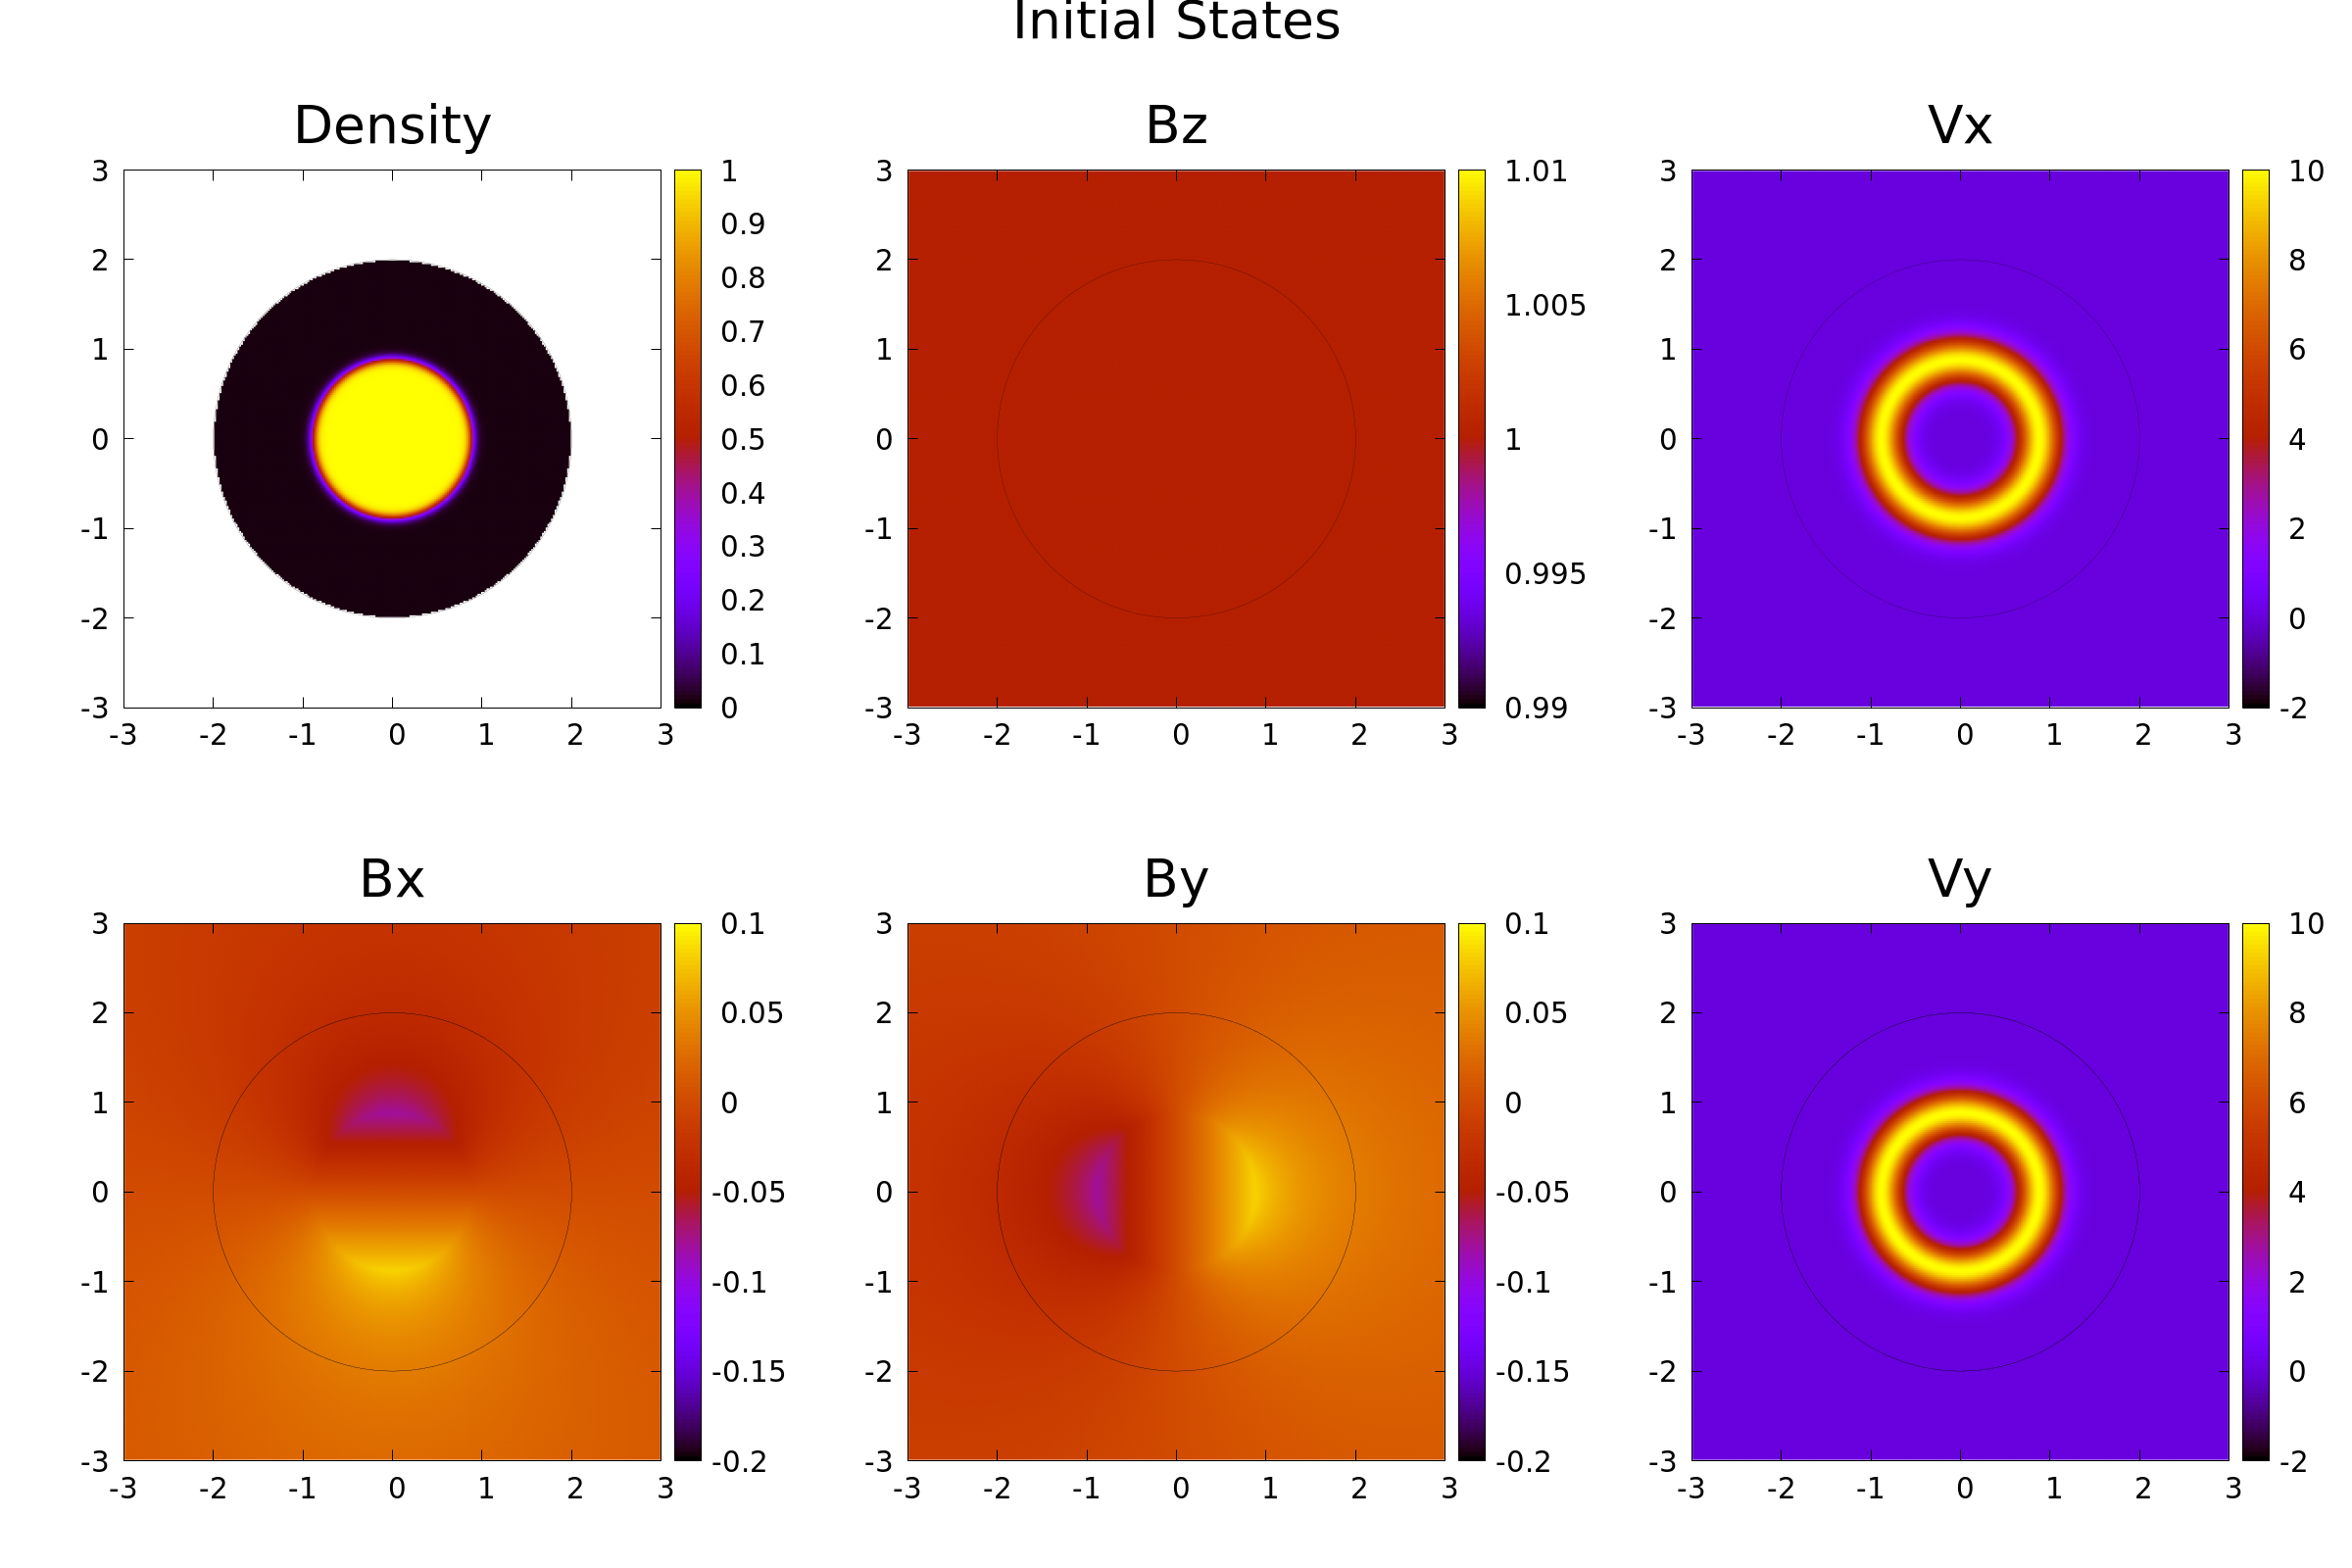
\includegraphics[width=1\linewidth]{InitialCylindricalEquilibrium.png}
	\caption[Initial states of cylindrical equilibrium]{Visualization of the initial states for cylindrical equilibrium. This test is built by Chrysanthou \cite{chrysanthou2020} based on some initial values from Ferraro \textit{et al.} \cite{ferraro2016multi}. The color box ranges are manually adjusted to make the features more obvious.}
	\label{fig:cylindricalEquilibriumInitial}
\end{figure}

After setting the initial states properly, the test is conducted within $300\times300$ resolution numerical area with $C_{CFL}=0.4$. Because of the possible stiffness of the resistive ODE, we use a low CFL number as an additional safety measure against numerical instabilities. The test is conducted to $t_{stop}=0.2$ after the core plasma hitting the boundary. Similar tests are conducted to make a comparison between perfect conducting condition $\eta_w=0.0$ and resistive condition $\eta_w=0.05$ as demonstrated in Figure \ref{fig:cylindricalEquilibrium}. 

The simulation results, depicted in Figure \ref{fig:cylindricalEquilibrium}, provide a comparison between the behavior of the system under perfect conducting walls (left column) and resistive walls with $\eta=0.05$ (right column). The two quantities examined are the plasma density (top row) and the magnetic field component $B_z$ (bottom row). While the overall behavior of the plasma appears similar across both boundary conditions, a notable difference emerges in the $B_z$ component. Under resistive conditions, the interaction between the plasma and the magnetic field within the rigid body leads to a significant increase in $B_z$.  This interaction causes the peak $B_z$ value within the plasma from 3.1758 in perfect conducting case to rise to 5.2921 in resistive case. On the other hand, changes in the plasma density are subtler, with only a slight increase in the peak density under resistive conditions, likely as a consequence of the magnetic field. In general, our result are in close qualitative agreement with Chrysanthou's results \cite{chrysanthou2020}.

\begin{figure}[H]
	\centering
	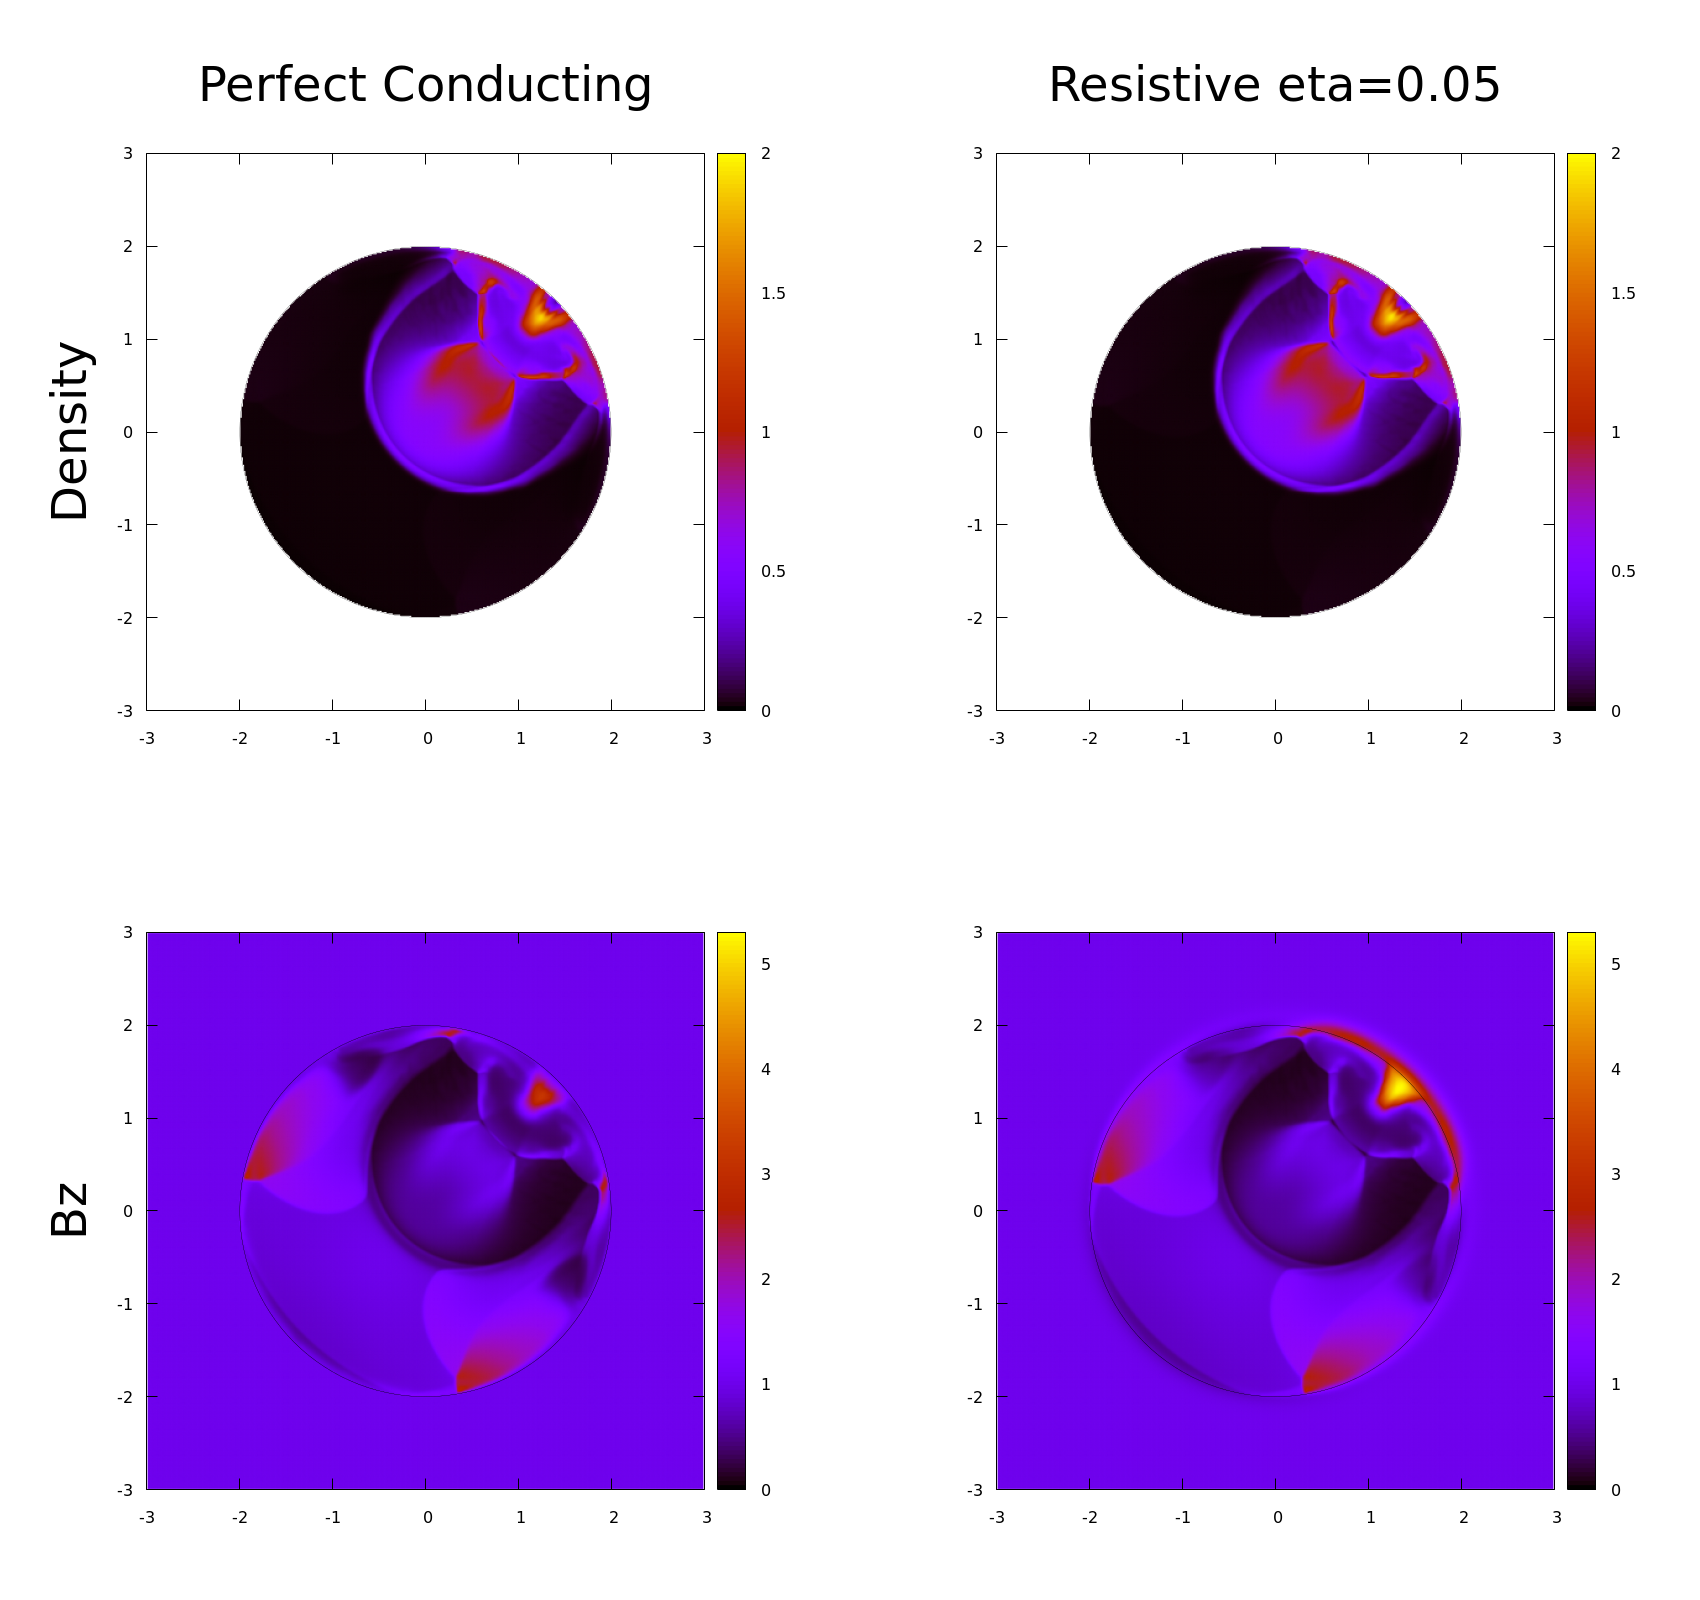
\includegraphics[width=1\linewidth]{cylindricalEquilibrium.png}
	\caption[Result of cylindrical equilibrium]{Results of the cylindrical equilibrium simulation. These plots compare the outcomes between a perfect conducting wall (left column) and a resistive wall $\eta=0.05$ (right column) with two key quantities, the plasma density (top row) and the magnetic field component $B_z$ (bottom row). Generally, they are similar in different boundary conditions. The primary difference is observed in the $B_z$ component. In the resistive scenario, the $B_z$ within the rigid body is significantly influenced by the plasma, leading to a noticeable increase. As a result, the peak $B_z$ value inside the plasma reaches 5.2921, compared to the 3.1758 peak in the perfect conducting case. However, the difference is hard to tell in density, except for a slight increase in the resistive density peak, which may be attributed to the influence of the magnetic field.}
	\label{fig:cylindricalEquilibrium}
\end{figure}

\subsubsection*{Total Energy}
Under ideal conditions, a perfect conducting wall should theoretically maintain a constant energy level within the system. However, the application of numerical methods such as the ghost fluid method can often lead to fluctuations or even reductions in total energy. When a resistive boundary condition is employed, the increase in resistivity allows more of the magnetic field to penetrate into the rigid body from the plasma. Consequently, the total energy within the plasma is expected to gradually decrease. To validate these hypotheses, we conducted a series of simulations. We accumulate the total energy over the whole plasma region and plot their curve as a function of time. The Figure \ref{fig:totalEnergy} below demonstrate temporal evolution of total energy. When $\eta_w=0.0$, the boundary condition used is the perfect conducting condition introduced in \ref{chapter 2}, the same as in the rotated Brio-Wu test; for $\eta_w>0.0$, the boundary condition is implemented by using the $\mathbf{B}$ values in the wall as ghost cells for the plasma, and vice versa, following the principles on wall outlined in equation \ref{equ:magneticDiffusion}. Overall, all the curves exhibit a downward trend. This may be attributed to the application of the ghost fluid method and the meshing revolution. As we incrementally increase $\eta_w$, the total final energy decreases, which aligns with our expectation that a more resistive wall allows greater magnetic field penetration, thereby reducing the total energy within the plasma. Furthermore, this decline appears to follow an exponential pattern. Although $\eta_w$ increases in fixed steps, the resulting decrease in total energy becomes progressively smaller. Notably, the gap between the curves for $\eta_w=0.0$ and $\eta_w=0.001$ is relatively large, potentially indicating the presence of some nonlinear behavior. This inconsistency will be discussed further in Chapter \ref{chapter 10}.

\begin{figure}[H]
	\centering
	\vspace{5mm}
	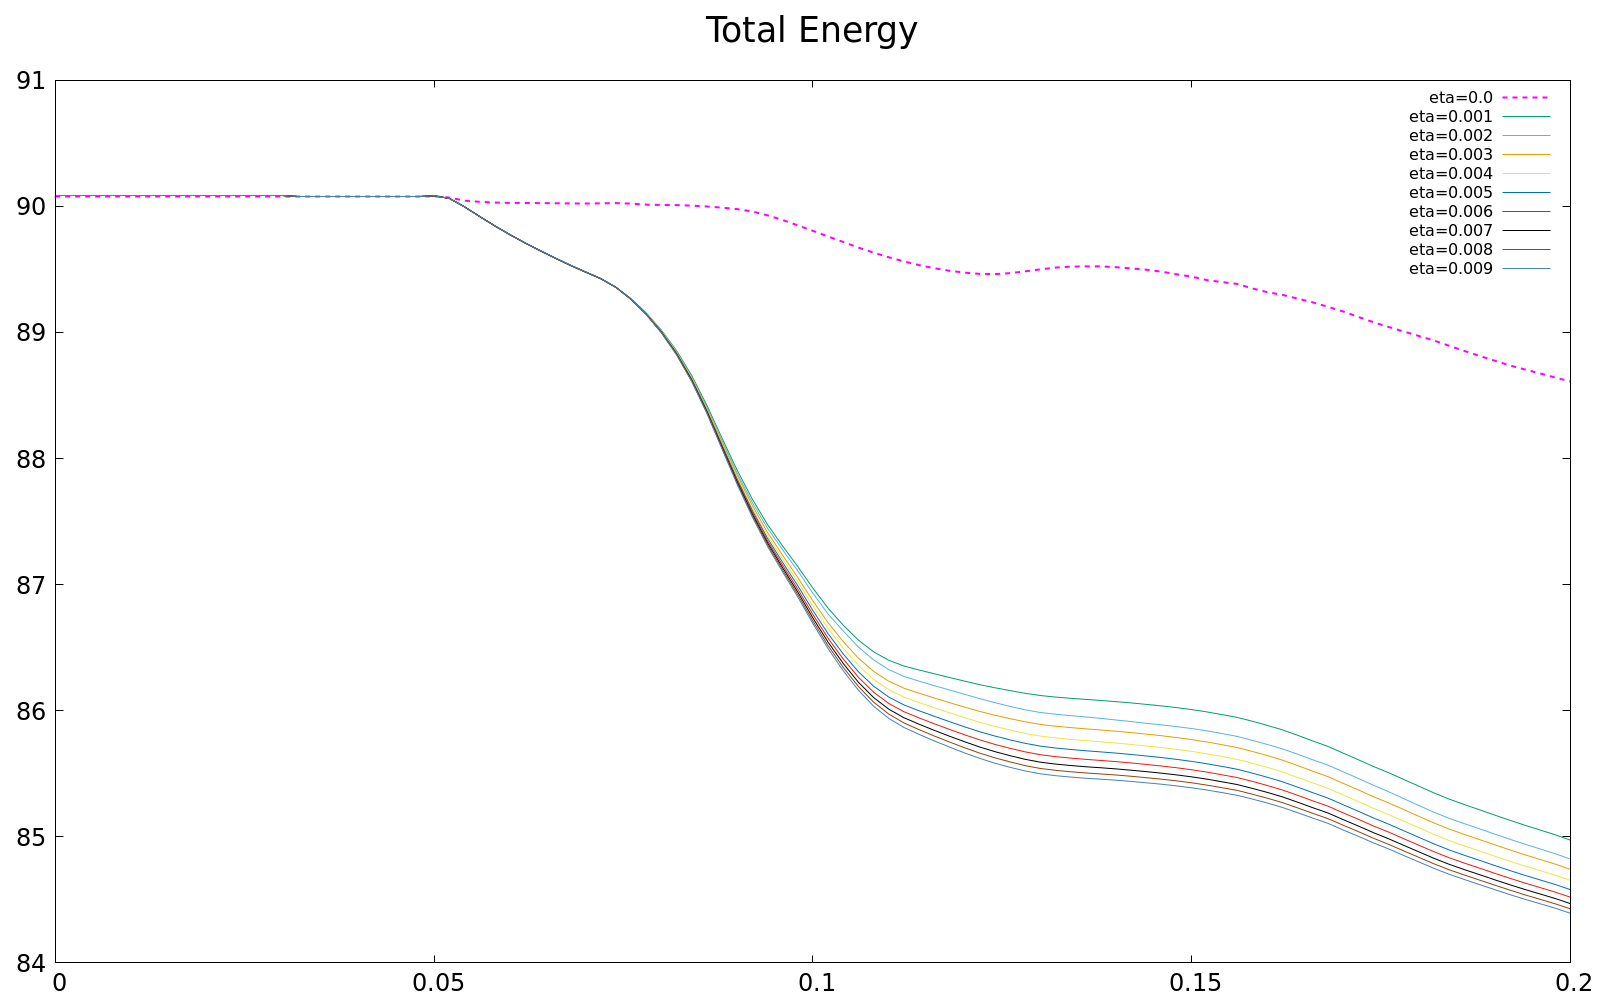
\includegraphics[width=1\linewidth]{TotalEnergy.png}
	\caption[Total energy curves]{This figure illustrates the temporal evolution of plasma total energy in the cylindrical equilibrium test, showing downward trends over time. As $\eta_w$ increases, the energy decreases further. The decline appears exponential, with diminishing energy reductions as $\eta_w$ increases.}
	\label{fig:totalEnergy}
\end{figure}



\section{Tokamak-shaped Application}
In earlier sections, the boundary conditions are validated and solvers with cylindrical equilibrium test. In this chapter, we apply this test in a container that more closely resembles a tokamak vessel. We build up a chamber similar to tokamak vessel in Ferraro \textit{et al.} \cite{ferraro2016multi}. We use tungsten as the vessel wall material. Hence, the resistivity is $5.6 \times 10^{-8} \, \Omega \cdot \text{m}$. The whole simulation is conducted under numerical domain of $[0.2,3.3]\times[-2.5,2.5]$ with $310\times500$ resolution. We extend the simulation to $t_{stop}=0.8$. 

The results are demonstrated in Figure \ref{fig:tokamak_application_inchapter9}. This simulation in the tokamak-shaped vessel provides valuable insights into the behavior of plasma under conditions that more closely resemble practical applications. As depicted in the figures, the simulation demonstrates the high-density plasma core impacting the tokamak wall. Upon impact, the plasma is observed to split and disperse along the wall. Unlike the cylindrical equilibrium test in the previous section, here, due to the very low resistivity of tungsten, the impact on the magnetic field when the wall is struck is hardly noticeable. It is also difficult to observe any significant plasma-wall interaction when the plasma moves along the boundary. After the initial impact, the more noticeable magnetic field fast magneto-acoustic waves are generated and propagate through the plasma. The figures show these waves spreading out from the impact region and interacting with other waves and structures within the vessel. They collide and interfere in the lower part of the vessel, which suggests the presence of non-linear wave interactions in the end of the simulation.


\begin{figure}[htbp]
	\centering
	
	\vspace{-5mm}
	% Row 1
	\hspace{-6mm}
	\begin{subfigure}{0.26\textwidth}
		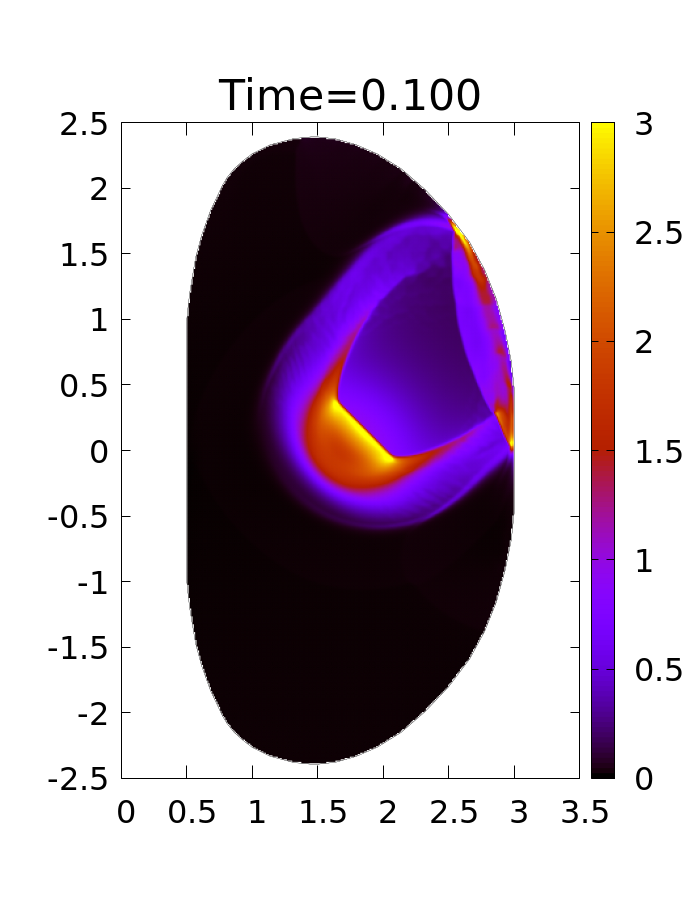
\includegraphics[width=\linewidth]{tokamak_Density_050.png}
	\end{subfigure}
	\hspace{-4mm} % Negative horizontal space
	\begin{subfigure}{0.26\textwidth}
		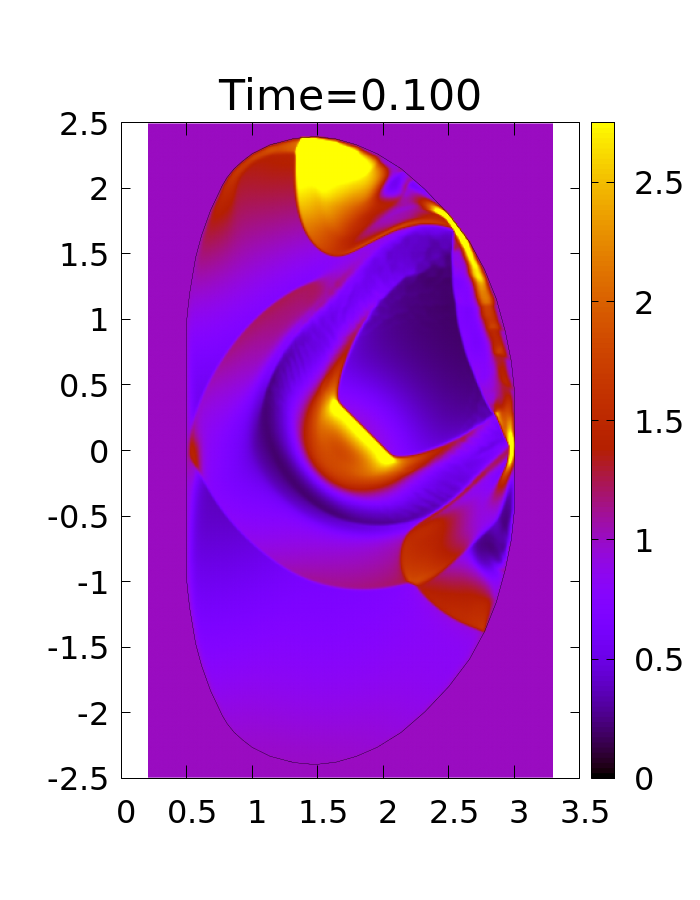
\includegraphics[width=\linewidth]{tokamak_Bz_050.png}
	\end{subfigure}
	\hspace{2mm} % Negative horizontal space
	\begin{subfigure}{0.26\textwidth}
		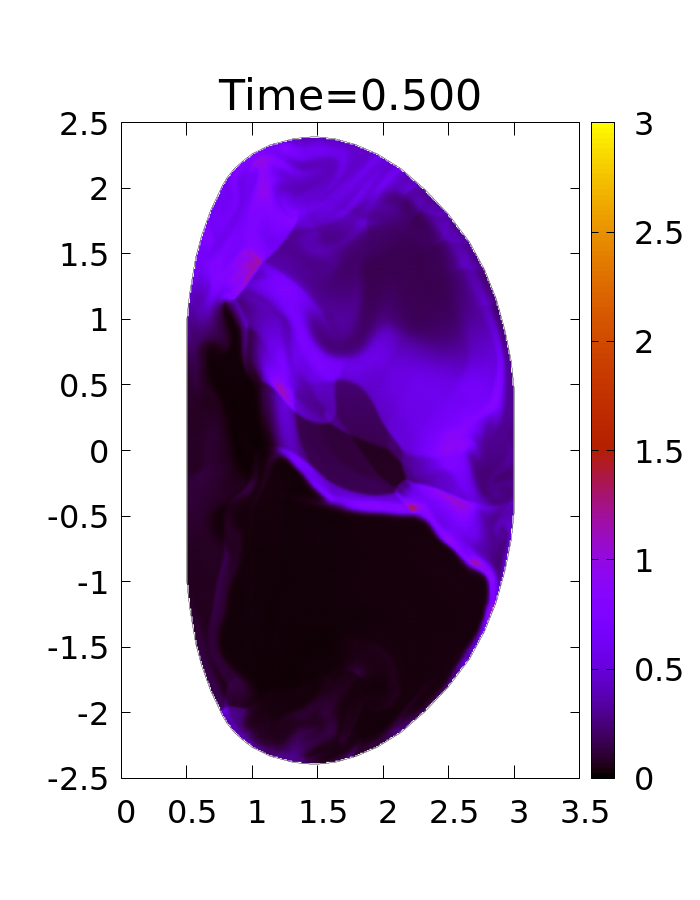
\includegraphics[width=\linewidth]{tokamak_Density_250.png}
	\end{subfigure}
	\hspace{-4mm} % Negative horizontal space
	\begin{subfigure}{0.26\textwidth}
		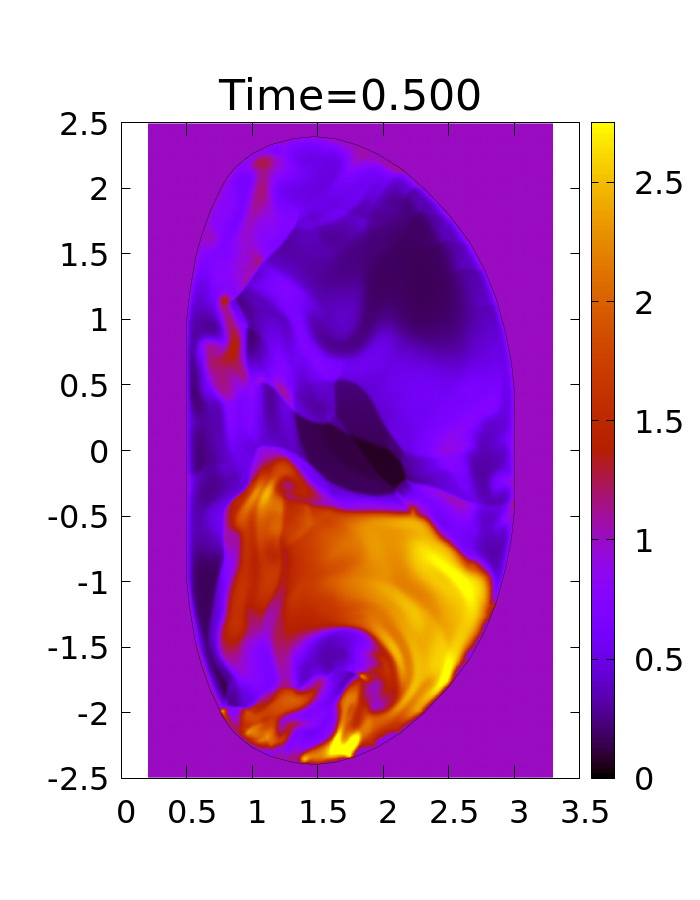
\includegraphics[width=\linewidth]{tokamak_Bz_250.png}
	\end{subfigure}
	\hspace{-6mm}
	
	\vspace{-6mm} % Negative vertical space
	
	% Row 2
	\hspace{-6mm}
	\begin{subfigure}{0.26\textwidth}
		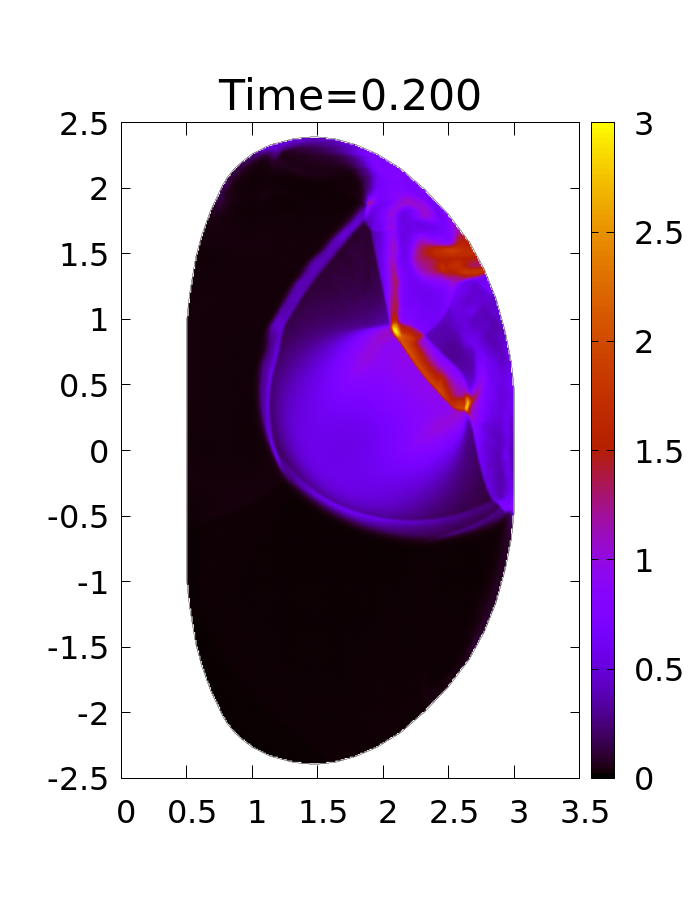
\includegraphics[width=\linewidth]{tokamak_Density_100.png}
	\end{subfigure}
	\hspace{-4mm} % Repeat negative space adjustments for each subfigure
	\begin{subfigure}{0.26\textwidth}
		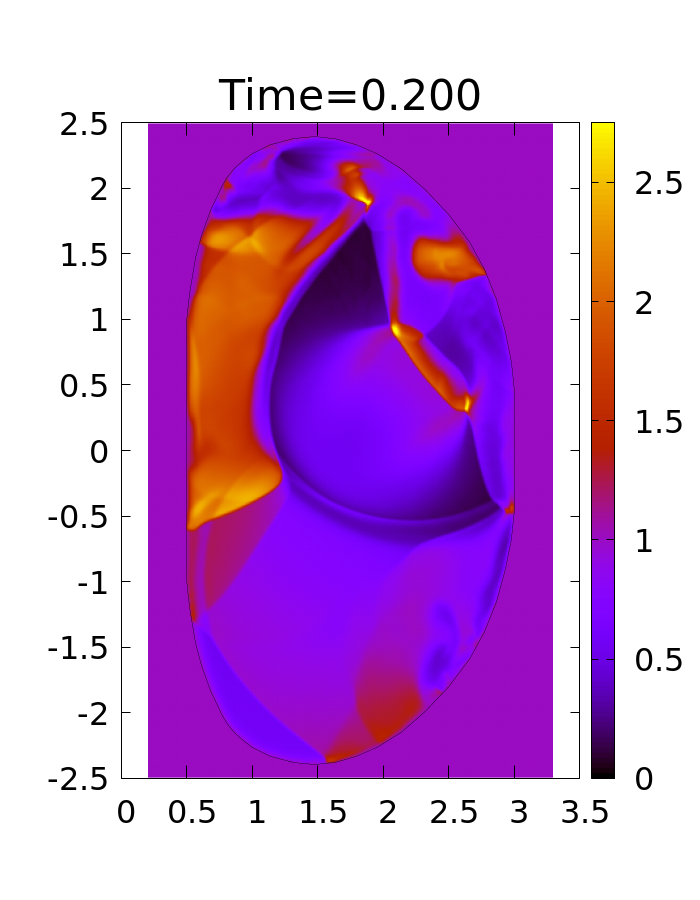
\includegraphics[width=\linewidth]{tokamak_Bz_100.png}
	\end{subfigure}
	\hspace{2mm} % Repeat negative space adjustments for each subfigure
	\begin{subfigure}{0.26\textwidth}
		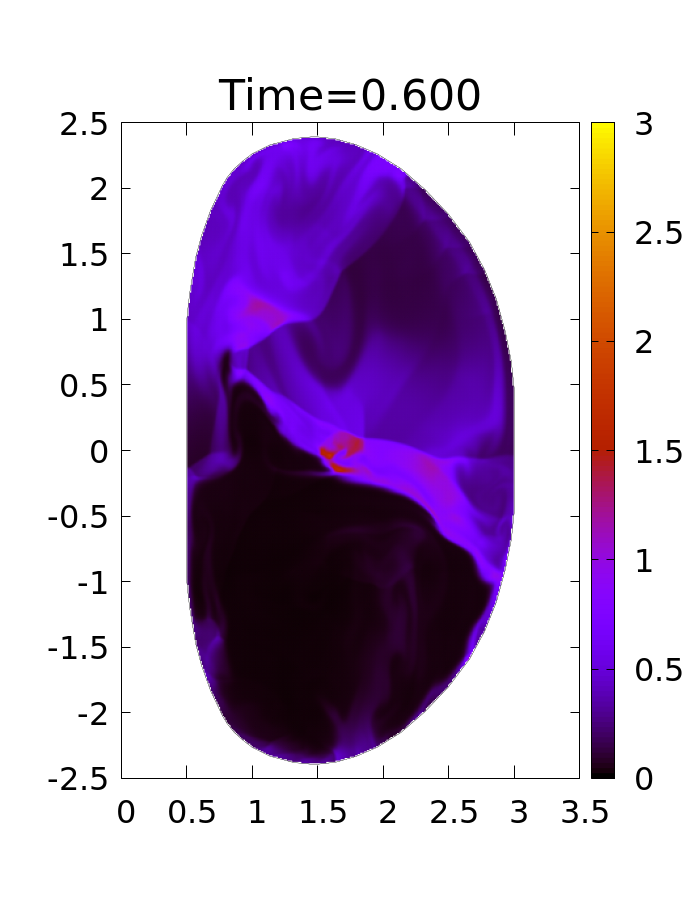
\includegraphics[width=\linewidth]{tokamak_Density_300.png}
	\end{subfigure}
	\hspace{-4mm} % Repeat negative space adjustments for each subfigure
	\begin{subfigure}{0.26\textwidth}
		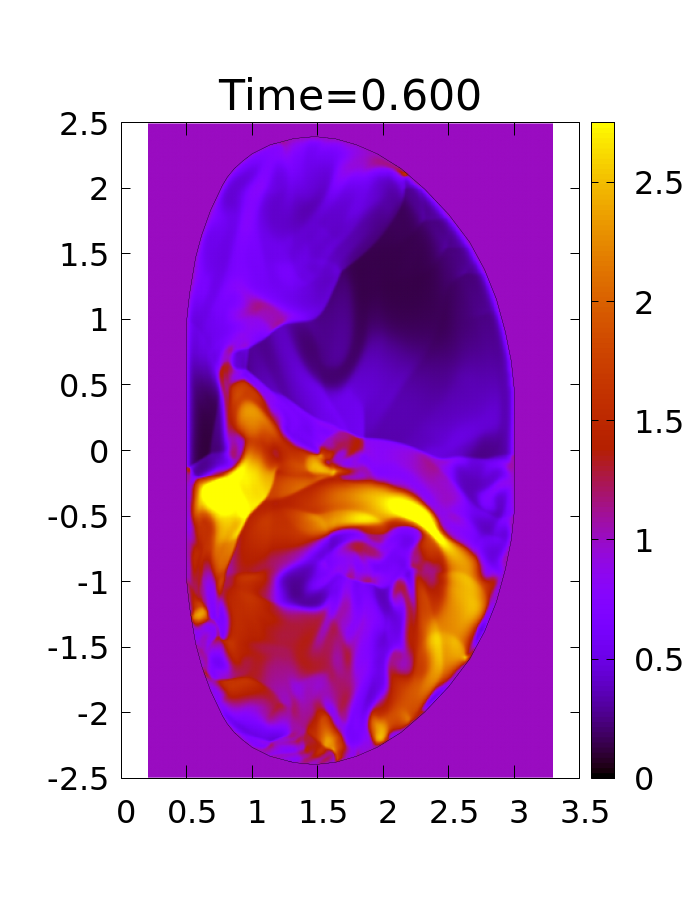
\includegraphics[width=\linewidth]{tokamak_Bz_300.png}
	\end{subfigure}
	\hspace{-5mm}
	
	\vspace{-6mm} % Negative vertical space
	
	% Row 3
	\hspace{-6mm}
	\begin{subfigure}{0.26\textwidth}
		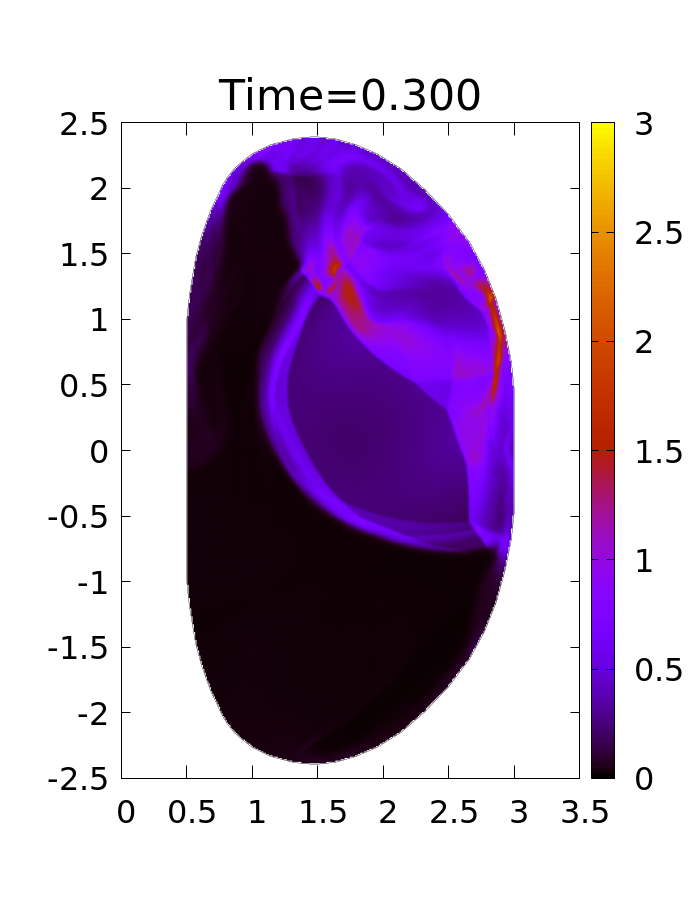
\includegraphics[width=\linewidth]{tokamak_Density_150.png}
	\end{subfigure}
	\hspace{-4mm} % Repeat negative space adjustments for each subfigure
	\begin{subfigure}{0.26\textwidth}
		\includegraphics[width=\linewidth]{tokamak_Bz_150.png}
	\end{subfigure}
	\hspace{2mm} % Repeat negative space adjustments for each subfigure
	\begin{subfigure}{0.26\textwidth}
		\includegraphics[width=\linewidth]{tokamak_Density_350.png}
	\end{subfigure}
	\hspace{-4mm} % Repeat negative space adjustments for each subfigure
	\begin{subfigure}{0.26\textwidth}
		\includegraphics[width=\linewidth]{tokamak_Bz_350.png}
	\end{subfigure}
	\hspace{-6mm}
	
	\vspace{-6mm} % Negative vertical space
	
	% Row 4 
	\hspace{-6mm}
	\begin{subfigure}{0.26\textwidth}
		\includegraphics[width=\linewidth]{tokamak_Density_200.png}
		\caption*{Density}
	\end{subfigure}
	\hspace{-4mm} % Repeat negative space adjustments for each subfigure
	\begin{subfigure}{0.26\textwidth}
		\includegraphics[width=\linewidth]{tokamak_Bz_200.png}
		\caption*{$B_z$}
	\end{subfigure}
	\hspace{2mm} % Repeat negative space adjustments for each subfigure
	\begin{subfigure}{0.26\textwidth}
		\includegraphics[width=\linewidth]{tokamak_Density_400.png}
		\caption*{Density}
	\end{subfigure}
	\hspace{-4mm} % Repeat negative space adjustments for each subfigure
	\begin{subfigure}{0.26\textwidth}
		\includegraphics[width=\linewidth]{tokamak_Bz_400.png}
		\caption*{$B_z$}
	\end{subfigure}
	\hspace{-6mm}
	
	\vspace{1mm} % Negative vertical space
	
	\caption[Tokamak Application]{Simulation of the cylindrical equilibrium test in a tokamak-shaped vessel. The wall is assumed to be made of tungsten, with a resistivity of $5.6 \times 10^{-8} \, \Omega \cdot \text{m}$.}
	\label{fig:tokamak_application_inchapter9}
\end{figure}


  

%%!TEX root = ../thesis.tex
%*******************************************************************************
%*********************************** First Chapter *****************************
%*******************************************************************************

\chapter{Tokamak-shape Application}  %Title of the First Chapter

\ifpdf
    \graphicspath{{Chapter9/Figs/Raster/}{Chapter9/Figs/PDF/}{Chapter9/Figs/}}
\else
    \graphicspath{{Chapter9/Figs/Vector/}{Chapter9/Figs/}}
\fi

\label{chapter 9}


%************************************************************************** 

In the last chapter, we validate the boundary conditions and solvers with cylindrical equilibrium test. In this chapter, we apply this test in a container that more closely resembles a tokamak vessel. We build up a chamber similar to tokamak vessel in Ferraro \textit{et al.} \cite{ferraro2016multi}. We use tungsten as the vessel wall material. Hence, the resistivity is $5.6 \times 10^{-8} \, \Omega \cdot \text{m}$. The whole simulation is conducted under numerical domain of $[0.2,3.3]\times[-2.5,2.5]$ with $310\times500$ resolution. We extend the simulation to $t_{stop}=0.8$. 

The result is demonstrated in Figure \ref{fig:tokamak_application}. This simulation in the tokamak-shaped vessel provide valuable insights into the behavior of plasma under conditions that more closely resemble practical applications. As depicted in the figures, the result demonstrate the procedure core high density plasma hitting the wall and splitting out. The interaction behavior of the fast magnetoacoustic wave is particularly interesting after they are generated during the hitting and spread out, they collide again in the lower part of the vessel.


\begin{figure}[htbp]
	\centering
	
	\vspace{-5mm}
	% Row 1
	\hspace{-6mm}
	\begin{subfigure}{0.26\textwidth}
		\includegraphics[width=\linewidth]{tokamak_Density_050.png}
	\end{subfigure}
	\hspace{-4mm} % Negative horizontal space
	\begin{subfigure}{0.26\textwidth}
		\includegraphics[width=\linewidth]{tokamak_Bz_050.png}
	\end{subfigure}
	\hspace{2mm} % Negative horizontal space
	\begin{subfigure}{0.26\textwidth}
		\includegraphics[width=\linewidth]{tokamak_Density_250.png}
	\end{subfigure}
	\hspace{-4mm} % Negative horizontal space
	\begin{subfigure}{0.26\textwidth}
		\includegraphics[width=\linewidth]{tokamak_Bz_250.png}
	\end{subfigure}
	\hspace{-6mm}
	
	\vspace{-6mm} % Negative vertical space
	
	% Row 2
	\hspace{-6mm}
	\begin{subfigure}{0.26\textwidth}
		\includegraphics[width=\linewidth]{tokamak_Density_100.png}
	\end{subfigure}
	\hspace{-4mm} % Repeat negative space adjustments for each subfigure
	\begin{subfigure}{0.26\textwidth}
		\includegraphics[width=\linewidth]{tokamak_Bz_100.png}
	\end{subfigure}
	\hspace{2mm} % Repeat negative space adjustments for each subfigure
	\begin{subfigure}{0.26\textwidth}
		\includegraphics[width=\linewidth]{tokamak_Density_300.png}
	\end{subfigure}
	\hspace{-4mm} % Repeat negative space adjustments for each subfigure
	\begin{subfigure}{0.26\textwidth}
		\includegraphics[width=\linewidth]{tokamak_Bz_300.png}
	\end{subfigure}
	\hspace{-5mm}
	
	\vspace{-6mm} % Negative vertical space
	
	% Row 3
	\hspace{-6mm}
	\begin{subfigure}{0.26\textwidth}
		\includegraphics[width=\linewidth]{tokamak_Density_150.png}
	\end{subfigure}
	\hspace{-4mm} % Repeat negative space adjustments for each subfigure
	\begin{subfigure}{0.26\textwidth}
		\includegraphics[width=\linewidth]{tokamak_Bz_150.png}
	\end{subfigure}
	\hspace{2mm} % Repeat negative space adjustments for each subfigure
	\begin{subfigure}{0.26\textwidth}
		\includegraphics[width=\linewidth]{tokamak_Density_350.png}
	\end{subfigure}
	\hspace{-4mm} % Repeat negative space adjustments for each subfigure
	\begin{subfigure}{0.26\textwidth}
		\includegraphics[width=\linewidth]{tokamak_Bz_350.png}
	\end{subfigure}
	\hspace{-6mm}
	
	\vspace{-6mm} % Negative vertical space
	
	% Row 4 
	\hspace{-6mm}
	\begin{subfigure}{0.26\textwidth}
		\includegraphics[width=\linewidth]{tokamak_Density_200.png}
		\caption*{Density}
	\end{subfigure}
	\hspace{-4mm} % Repeat negative space adjustments for each subfigure
	\begin{subfigure}{0.26\textwidth}
		\includegraphics[width=\linewidth]{tokamak_Bz_200.png}
		\caption*{$B_z$}
	\end{subfigure}
	\hspace{2mm} % Repeat negative space adjustments for each subfigure
	\begin{subfigure}{0.26\textwidth}
		\includegraphics[width=\linewidth]{tokamak_Density_400.png}
		\caption*{Density}
	\end{subfigure}
	\hspace{-4mm} % Repeat negative space adjustments for each subfigure
	\begin{subfigure}{0.26\textwidth}
		\includegraphics[width=\linewidth]{tokamak_Bz_400.png}
		\caption*{$B_z$}
	\end{subfigure}
	\hspace{-6mm}
	
	\vspace{1mm} % Negative vertical space
		
	\caption[Tokamak Application]{Simulation of cylindrical equilibrium test in a tokamak-shaped vessel. Assume the wall material is tungsten, with a resistivity of $5.6 \times 10^{-8} \, \Omega \cdot \text{m}$.}
	\label{fig:tokamak_application}
\end{figure} 


  

%!TEX root = ../thesis.tex
%*******************************************************************************
%*********************************** First Chapter *****************************
%*******************************************************************************

\chapter{Consistency}  %Title of the First Chapter

\ifpdf
    \graphicspath{{Chapter10/Figs/Raster/}{Chapter10/Figs/PDF/}{Chapter10/Figs/}}
\else
    \graphicspath{{Chapter10/Figs/Vector/}{Chapter10/Figs/}}
\fi

\label{chapter 10}


%************************************************************************** 

A reflective Dirichlet boundary condition is validated for perfect conducting wall in rotated Brio-Wu test in chapter \ref{chapter 4}, based on Dirichlet boundary condition suggested by Sambasivan and UdayKumar \cite{sambasivan2009ghost}. The resistive boundary condition represented by equation \ref{equ:magneticDiffusion} is applied in cylindrical equilibrium in chapter \ref{chapter 8}, similar to most of resistive wall relevant papers \cite{chrysanthou2020,ferraro2016multi,becerra2016resistive,hender1989effects}. These methods are all mainstream methods. Yet, it seems that when the resistivity approaches zero, it's still quite different from when the resistivity is exactly zero, as shown in Figure \ref{fig:totalEnergy}. In this chapter, we are going to analyze superconducting wall condition and extend these into a general wall condition, which may help to address this inconsistency.

\section{Superconducting Wall Condition}
\subsection{London Equations and Meissner Effect}
We start from some basic theories of London Equations. London Equations are relevant to Meissner effect in superconductors \cite{london_equations_wikipedia}. The Meissner effect is the phenomenon where a superconductor expels magnetic fields from its interior when it transitions into the superconducting state. We focus on the London equations and the reasoning behind their derivation.

It starts from the definition of current density. The current density is defined as 
$$
\mathbf{J}_s=-n_s q_e \mathbf{v}_s\ ,
$$
Where the $q_e$ is the elementary charge on a single electron with  $q_e=-1.602176634\times10^{-19}$, a negative number. The $n_s$ and $\mathbf{v}_s$, in simple terms, are electron number density and velocity, where lower index $s$ specify a superconductor situation. We have the Newton's Second Law of Motion for electron
\begin{equation}
m\frac{d\mathbf{v}_s}{dt}=-q_e\mathbf{E}\ ,
\label{equ:motion_perfectConducting}
\end{equation}
where $m$ is the electron mass and $\mathbf{E}$ is the electric field. By getting the time derivative of current density $\mathbf{J}_s$ and substituting velocity derivative over time with equation \ref{equ:motion_perfectConducting}, it gives the London First Equation
$$
\frac{\partial \mathbf{J}_s}{\partial t}=\frac{n_s q_e^2}{m}\mathbf{E}\ .
$$
This describe the relationship in a superconductor, electric field accelerate electrons and increase the current density. By taking a curl on both sides and substituting the $\nabla\times\mathbf{E}=-\frac{\partial \mathbf{B}}{\partial t}$ with Faraday's law, it gives
$$
\frac{\partial }{\partial t}\left(\nabla\times\mathbf{J}_s+\frac{n_s q_e^2}{m}\mathbf{B}\right)=0\ .
$$

From the Meissner effect, it is found that $\mathbf{B}=0$ holds for all superconductor and $\nabla\times\mathbf{J}_s$ can not be a non-zero constant. It gives the London Second Equation
$$
\nabla\times\mathbf{J}_s+\frac{n_s q_e^2}{m}\mathbf{B}=0\ .
$$
Further replacing current density by static condition of Ampere's Law, $\mathbf{J}_s=\nabla \times \mathbf{B}$, this give a equation that only contain magnetic field. Along with identity $\nabla\times\nabla\times\mathbf{B}=\nabla\left(\nabla\cdot\mathbf{B}\right)-\nabla^2\mathbf{B}$, while $\nabla\cdot\mathbf{B}=0$, these give \cite{london_equations_wikipedia} 
\begin{equation}
	\nabla^2\mathbf{B}=\frac{1}{\lambda_s^2}\mathbf{B}\ ,\ \ \ \ \ \  \lambda_s^2=\frac{m}{n_s q_e^2}\ .
	\label{equ:B_superconducting}
\end{equation}


\subsection{Penetration on Superconductor Wall}
This equation \ref{equ:B_superconducting} give us some information on magnetic field within superconductors. If we place a magnetic field, we may know about the strength distribution and how the superconducting wall reflect the normal component of magnetic field. We place a wall in vacuum. As depicted in Plot \ref{fig:magneticPenetration}, a normal magnetic $\mathbf{B}=B_0\mathbf{i}$ is imposed on the wall suddenly. The x dimension is the only mattering direction. This give a equation along x.
\begin{equation}
	\frac{\partial^2 B_x}{\partial x^2}=\frac{1}{\lambda_s^2}B_x\ .
\end{equation}
It is a homogeneous second order differential equation, a Helmholtz equation \cite{london_equations_wikipedia}. A general solution can be given as $B_x(x)=C_1e^{\frac{x}{\lambda_s}}+C_2e^{-\frac{x}{\lambda_s}}$. Some physical boundary conditions are given as $B_x(0)=B_0$ and $\lim_{x \to \infty} B_x(x)=0$. These define the solution
\begin{equation}
	B_x(x)=B_0e^{-\frac{x}{\lambda_s}}\ .
\end{equation}
$\lambda_s$ is 'penetration depth' controlling the penetration. Even for superconductors, there will be some penetration. As discussed in chapter \ref{chapter 6}, the superconducting materials used in ITER and EAST are Nb3Sn and NbTi. Their penetration depths are around $\lambda_{Nb3Sn}=8.0\times10^{-8}m$ and $\lambda_{NbTi}=1.0\times10^{-7}m$. For a better visualization, we add a simple case    $\lambda_{0}=4.6\times10^{-4}m$ based on the relevant parameter on tungsten \cite{greiner2012classical}. Their penetrations under simply $B_0=1.0$ are demonstrated in Figure \ref{fig:PenetrationCurveSuperconducting}. After penetrating into a superconducting wall, the magnetic field is fully countered off. This form a 'no-penetration' condition on normal magnetic field. A reflective boundary is applied on this condition. We proved these mathematically in chapter \ref{chapter 2}. 
 
\begin{figure}[H]
	\centering
	\includegraphics[width=0.8\linewidth]{BPenetration.png}
	\caption[Magnetic Penetration]{An illustration of normal magnetic field on a conducting wall. The entire space is divided into two parts: the left side ($x<0$) is a vacuum, and the right side ($x\geq0$) is a wall made of a certain conductor material. A homogeneous normal magnetic field $\mathbf{B}=B_0\mathbf{i}$ is suddenly imposed on the wall. The extent to which the magnetic field penetrates the wall depends on the resistivity of the wall's material.}
	\label{fig:magneticPenetration}
\end{figure}

\begin{figure}[H]
	\centering
	\includegraphics[width=1\linewidth]{penetration_superconducting.png}
	\caption[Bx Distribution]{Magnetic penetration along x.}
	\label{fig:PenetrationCurveSuperconducting}
\end{figure}

\section{Extension on General Wall}
We make an extension into a general wall condition. A similar relationship still hold for current density based on free number density $n$,  
$$
\mathbf{J}=-n q_e \mathbf{v}\ .
$$
However, in the Newton's Second Law of Motion, we need to consider the effect of resistivity. In microscopic point of view, electron collides when moving along conductor. We use collision frequency $\nu$ to represent such phenomenon. The resistivity $\eta_w$ and $\nu$ have relation $\eta_w=\frac{nq_e^2}{\nu m}$. In Kittle \cite{kittel2018introduction}, a similar collision time $\tau$ and conductivity are defined. From a macroscopic perspective, this behaves like damping \cite{kittel2018introduction}. The motion of electron can be given by 
$$
m\frac{d\mathbf{v}}{dt}+m\nu \mathbf{v}=-q_eE\ .
$$

Solving this differential equation for $\mathbf{v}$ along with a initial condition $\mathbf{v}_0=0$, give the solution 
$$
\mathbf{v}=-\frac{q_e\mathbf{E}}{\nu m}+\frac{q_e\mathbf{E}}{\nu m}e^{-\nu t}\ .
$$

After taking curl and applying the Faraday's Law, we rearrange the equation and substitute some terms with $\eta_w$. These give the equation
\begin{equation}
	\nabla^2\mathbf{B}=\frac{nq_e^2}{m\nu}\frac{\partial \mathbf{B}}{\partial t}-\frac{nq_e^2}{m\nu}e^{-\nu t}\frac{\partial \mathbf{B}}{\partial t}
\end{equation}

\section{Boundary Condition Recap} 
This equation gives a more consistent resistive boundary condition rather than equation \ref{equ:magneticDiffusion}.
\subsection*{Perfect Conducting Wall}
For perfect conducting wall, L'Hopital's Rule gives $$
\lim_{\nu \to 0}\frac{1-e^{-\nu t}}{\nu}=\frac{\frac{\partial(1-e^{-\nu t})}{\partial t}}{\frac{\partial\nu}{\partial t}}=-t\ .
$$ 
With a perturbation method applied, the change over time is small and approximately linear $t\frac{\partial \mathbf{B}}{\partial t}\approx\mathbf{B}$. It gives 
$$
\nabla^2\mathbf{B}=\frac{n q_e^2}{m}\mathbf{B}\ .
$$
This is the same as discussed in superconducting case. We have shown that a reflective Dirichlet boundary condition is appropriate in this case.

\subsection*{Resistive Wall and Insulator Wall}
For a resistive wall, $\nu$ is big and $e^{-\nu t}$ can be ignored. With relation $\eta_w=\frac{nq_e^2}{\nu m}$, we have 
$$
\eta_{w}\nabla^2\mathbf{B}=\frac{\partial \mathbf{B}}{\partial t}\ .
$$
This is exactly the case we use in resistive wall in equation \ref{equ:magneticDiffusion_rearrange}. We deal with this boundary condition by updating it using some similar ghost fluid methods. These give results in earlier chapters. Insulator wall is just an extreme case of this situation. It is more convenient to just set it to be Neumann.

\subsection*{Small Resistivity}
In the Plot \ref{fig:totalEnergy}, the inconsistency happens when 
$$
\lim_{\nu \to 0,\eta_w \to 0}\ Resistive\ Wall \neq Perfect\ Conducting\ Wall\ .
$$
This equation enable us to know more about the situation when resistivity get close to 0 but not 0. We have series expansion of $e^{-\nu t}=\sum_{n=0}^{\infty}\frac{1}{n!}\nu^nt^n$. With the assumption that magnetic field change slightly over time and $\nu$ is small, t$\frac{\partial \mathbf{B}e^{-\nu t}}{\partial t}\approx\mathbf{B}e^{-\nu t}$. These give the equation 
\begin{equation*}
	\nabla^2\mathbf{B}=\frac{e^{-\nu t}}{\lambda^2}\mathbf{B}\ ,\ \ \ \ \ \  \lambda^2=\frac{m}{n q_e^2}\ .
\end{equation*}
A solution on x coordinate is
\begin{equation}
	B_x(x)=B_0e^{-\frac{xe^{-\frac{\nu t}{2}}}{\lambda}}\ .
\end{equation}

Figure \ref{fig:smallResistivityWall} demonstrate some visualization of this solution. For simplicity, we use $\nu=1.0$ and $\lambda_{0}=4.6\times10^{-4}m$. It seems that when the normal magnetic component impose on the small resistive wall, it react like a perfect conducting wall as in superconducting situation. The only effect of resistivity is to gradually allow the magnetic field to penetrate the wall over time. Based on the numerical methods we have, it seems that using a reflective boundary condition for the plasma while updating the rigid body magnetic field provides a better approximation for the boundary case with small resistivity.  

\begin{figure}[H]
	\centering
	\includegraphics[width=1\linewidth]{penetration_wall.png}
	\caption[Bx distribution on resistive wall]{Magnetic distribution on a resistive wall. When a normal magnetic field is applied to a small resistive wall, the initial magnetic field distribution inside behaves as if it were in a perfect conductor. However, the resistivity causes the magnetic field to slowly penetrate the wall over time.}
	\label{fig:smallResistivityWall}
\end{figure}
\section{Addressing the Inconsistency}
Generally, the inconsistency happens when $\lim_{\eta_w \to 0}$. This is because we only consider a damping effect on electrons when $\eta_w>0$ in Maxwell's equation of $\eta_w\mathbf{J}=\mathbf{E}$. However, for $\eta_w=0$, acceleration is the only factor considered. For example, in London Equations $m\frac{d\mathbf{v}_s}{dt}=-q_e\mathbf{E}$, where the electric field accelerates electrons infinitely. Hence, inconsistency occurs when neither of these effects can dominate $\lim_{\eta_w \to 0}$. There may be methods addressing this inconsistency by considering both effects in boundary condition, such as the Robin boundary condition proposed by Strauss \cite{strauss2014velocity}.  
%!TEX root = ../thesis.tex
%*******************************************************************************
%*********************************** First Chapter *****************************
%*******************************************************************************

\chapter{Summary}  %Title of the First Chapter

\ifpdf
    \graphicspath{{Chapter11/Figs/Raster/}{Chapter11/Figs/PDF/}{Chapter11/Figs/}}
\else
    \graphicspath{{Chapter11/Figs/Vector/}{Chapter11/Figs/}}
\fi

\label{chapter 11}


%************************************************************************** 

  The second report extends the work from the first report by focusing on the resistive wall conditions within tokamaks. The report begins with a review of the ideal Magnetohydrodynamics (MHD) model and highlights the transition from perfect conducting wall conditions to resistive wall conditions. Subsequently, the numerical methods and simulations are adapted to account for the resistivity of materials used in tokamak walls. These methods are validated through a series of computational tests, with comparisons drawn against results obtained under the assumption of a perfectly conducting wall, and are subsequently applied in a simulation within a tokamak-shaped vessel. The report concludes with a discussion on the limitations of electromagnetic dynamics. These findings may provide a more accurate boundary condition for resistive walls. Future studies could potentially propose a more consistent boundary condition that applies across insulator walls, resistive walls, small resistivity walls and perfect conducting walls.



% ********************************** Back Matter *******************************
% Backmatter should be commented out, if you are using appendices after References
%\backmatter

% ********************************** Bibliography ******************************
\begin{spacing}{0.9}

% To use the conventional natbib style referencing
% Bibliography style previews: http://nodonn.tipido.net/bibstyle.php
% Reference styles: http://sites.stat.psu.edu/~surajit/present/bib.htm

\bibliographystyle{apalike}
%\bibliographystyle{unsrt} % Use for unsorted references  
%\bibliographystyle{plainnat} % use this to have URLs listed in References
\cleardoublepage
\bibliography{References/references} % Path to your References.bib file


% If you would like to use BibLaTeX for your references, pass `custombib' as
% an option in the document class. The location of 'reference.bib' should be
% specified in the preamble.tex file in the custombib section.
% Comment out the lines related to natbib above and uncomment the following line.

%\printbibliography[heading=bibintoc, title={References}]


\end{spacing}

% ********************************** Appendices ********************************

\begin{appendices} % Using appendices environment for more functunality

% %!TEX root = ../thesis.tex
% ******************************* Thesis Appendix A ****************************
\chapter{How to install \LaTeX} 

\section*{Windows OS}

\subsection*{TeXLive package - full version}
\begin{enumerate}
\item	Download the TeXLive ISO (2.2GB) from\\
\href{https://www.tug.org/texlive/}{https://www.tug.org/texlive/}
\item	Download WinCDEmu (if you don't have a virtual drive) from \\
\href{http://wincdemu.sysprogs.org/download/}
{http://wincdemu.sysprogs.org/download/}
\item	To install Windows CD Emulator follow the instructions at\\
\href{http://wincdemu.sysprogs.org/tutorials/install/}
{http://wincdemu.sysprogs.org/tutorials/install/}
\item	Right click the iso and mount it using the WinCDEmu as shown in \\
\href{http://wincdemu.sysprogs.org/tutorials/mount/}{
http://wincdemu.sysprogs.org/tutorials/mount/}
\item	Open your virtual drive and run setup.pl
\end{enumerate}

or

\subsection*{Basic MikTeX - \TeX~ distribution}
\begin{enumerate}
\item	Download Basic-MiK\TeX (32bit or 64bit) from\\
\href{http://miktex.org/download}{http://miktex.org/download}
\item	Run the installer 
\item	To add a new package go to Start >> All Programs >> MikTex >> Maintenance (Admin) and choose Package Manager
\item	Select or search for packages to install
\end{enumerate}

\subsection*{TexStudio - \TeX~ editor}
\begin{enumerate}
\item	Download TexStudio from\\
\href{http://texstudio.sourceforge.net/\#downloads}
{http://texstudio.sourceforge.net/\#downloads} 
\item	Run the installer
\end{enumerate}

\section*{Mac OS X}
\subsection*{MacTeX - \TeX~ distribution}
\begin{enumerate}
\item	Download the file from\\
\href{https://www.tug.org/mactex/}{https://www.tug.org/mactex/}
\item	Extract and double click to run the installer. It does the entire configuration, sit back and relax.
\end{enumerate}

\subsection*{TexStudio - \TeX~ editor}
\begin{enumerate}
\item	Download TexStudio from\\
\href{http://texstudio.sourceforge.net/\#downloads}
{http://texstudio.sourceforge.net/\#downloads} 
\item	Extract and Start
\end{enumerate}


\section*{Unix/Linux}
\subsection*{TeXLive - \TeX~ distribution}
\subsubsection*{Getting the distribution:}
\begin{enumerate}
\item	TexLive can be downloaded from\\
\href{http://www.tug.org/texlive/acquire-netinstall.html}
{http://www.tug.org/texlive/acquire-netinstall.html}.
\item	TexLive is provided by most operating system you can use (rpm,apt-get or yum) to get TexLive distributions
\end{enumerate}

\subsubsection*{Installation}
\begin{enumerate}
\item	Mount the ISO file in the mnt directory
\begin{verbatim}
mount -t iso9660 -o ro,loop,noauto /your/texlive####.iso /mnt
\end{verbatim}

\item	Install wget on your OS (use rpm, apt-get or yum install)
\item	Run the installer script install-tl.
\begin{verbatim}
	cd /your/download/directory
	./install-tl
\end{verbatim}
\item	Enter command `i' for installation

\item	Post-Installation configuration:\\
\href{http://www.tug.org/texlive/doc/texlive-en/texlive-en.html\#x1-320003.4.1}
{http://www.tug.org/texlive/doc/texlive-en/texlive-en.html\#x1-320003.4.1} 
\item	Set the path for the directory of TexLive binaries in your .bashrc file
\end{enumerate}

\subsubsection*{For 32bit OS}
For Bourne-compatible shells such as bash, and using Intel x86 GNU/Linux and a default directory setup as an example, the file to edit might be \begin{verbatim}
edit $~/.bashrc file and add following lines
PATH=/usr/local/texlive/2011/bin/i386-linux:$PATH; 
export PATH 
MANPATH=/usr/local/texlive/2011/texmf/doc/man:$MANPATH;
export MANPATH 
INFOPATH=/usr/local/texlive/2011/texmf/doc/info:$INFOPATH;
export INFOPATH
\end{verbatim}
\subsubsection*{For 64bit OS}
\begin{verbatim}
edit $~/.bashrc file and add following lines
PATH=/usr/local/texlive/2011/bin/x86_64-linux:$PATH;
export PATH 
MANPATH=/usr/local/texlive/2011/texmf/doc/man:$MANPATH;
export MANPATH 
INFOPATH=/usr/local/texlive/2011/texmf/doc/info:$INFOPATH;
export INFOPATH

\end{verbatim}



%\subsection{Installing directly using Linux packages} 
\subsubsection*{Fedora/RedHat/CentOS:}
\begin{verbatim} 
sudo yum install texlive 
sudo yum install psutils 
\end{verbatim}


\subsubsection*{SUSE:}
\begin{verbatim}
sudo zypper install texlive
\end{verbatim}


\subsubsection*{Debian/Ubuntu:}
\begin{verbatim} 
sudo apt-get install texlive texlive-latex-extra 
sudo apt-get install psutils
\end{verbatim}

% %!TEX root = ../thesis.tex
% ******************************* Thesis Appendix B ********************************

\chapter{Installing the CUED class file}

\LaTeX.cls files can be accessed system-wide when they are placed in the
<texmf>/tex/latex directory, where <texmf> is the root directory of the user’s \TeX installation. On systems that have a local texmf tree (<texmflocal>), which
may be named ``texmf-local'' or ``localtexmf'', it may be advisable to install packages in <texmflocal>, rather than <texmf> as the contents of the former, unlike that of the latter, are preserved after the \LaTeX system is reinstalled and/or upgraded.

It is recommended that the user create a subdirectory <texmf>/tex/latex/CUED for all CUED related \LaTeX class and package files. On some \LaTeX systems, the directory look-up tables will need to be refreshed after making additions or deletions to the system files. For \TeX Live systems this is accomplished via executing ``texhash'' as root. MIK\TeX users can run ``initexmf -u'' to accomplish the same thing.

Users not willing or able to install the files system-wide can install them in their personal directories, but will then have to provide the path (full or relative) in addition to the filename when referring to them in \LaTeX.



\end{appendices}

% *************************************** Index ********************************
\printthesisindex % If index is present

\end{document}
